% Retoca las líneas marcadas con TODO según las necesidades

\documentclass[oneside,a4paper,12pt]{book} % TODO: cambia "oneside" por "twoside" a la hora de imprimirlo

\usepackage[spanish]{babel}
\usepackage[utf8]{inputenc}
\usepackage{geometry}
\usepackage{makeidx}
\usepackage{url}
\usepackage{graphicx}
\usepackage{color}
\usepackage{caption}
\usepackage{acronym}
\usepackage{hyphenat}
\usepackage{a4wide}
\usepackage[normalsize]{subfigure}
\usepackage{float}
\usepackage{titlesec}
\usepackage[export]{adjustbox}
\usepackage[Lenny]{fncychap}
\usepackage{listings} % para poder hacer uso de "listings" propios (p.ej. códigos)
\usepackage{eurosym} % para poder usar el símbolo del euro con \euro {xx}
\usepackage{hyperref} % TODO: añade la opción hidelinks para imprimirlo (los enlaces no aparecerán resaltados)

% Para que no parta las palabras
\pretolerance=10000

\newcommand{\bigrule}{\titlerule[0.5mm]} \titleformat{\chapter}[display] % cambiamos el formato de los capítulos
{\bfseries\Huge} % por defecto se usaron caracteres de tamaño huge en negrita
{% contenido de la etiqueta 
\titlerule % línea horizontal 
\filright % texto alineado a la derecha 
\Large\chaptertitlename\ % capítulo e índice en tamaño large
\Large % en lugar de 
\Huge \Large\thechapter} 
{0mm} % espacio mínimo entre etiqueta y cuerpo
{\filright} % texto del cuerpo alineado a la derecha
[\vspace{0.5mm} \bigrule] % después del cuerpo, dejar espacio vertical y trazar línea horizontal gruesa
\geometry{a4paper, left=3.5cm, right=2cm, top=3cm, bottom=2cm, headsep=1.5cm}

% Estilos para ilustrar códigos:
\definecolor{code_green}{rgb}{0,0.6,0}
\definecolor{code_gray}{rgb}{0.5,0.5,0.5}
\definecolor{code_mauve}{rgb}{0.58,0,0.82}

\lstset{frame=tb,
  language=C,
  aboveskip=3mm,
  belowskip=3mm,
  showstringspaces=false,
  columns=flexible,
  basicstyle={\small\ttfamily},
  numbers=none,
  numberstyle=\tiny\color{code_gray},
  keywordstyle=\color{blue},
  commentstyle=\color{code_green},
  stringstyle=\color{code_mauve},
  breaklines=true,
  breakatwhitespace=true,
  tabsize=3
}

\lstset{frame=tb,
  language=C++,
  aboveskip=3mm,
  belowskip=3mm,
  showstringspaces=false,
  columns=flexible,
  basicstyle={\small\ttfamily},
  numbers=none,
  numberstyle=\tiny\color{code_gray},
  keywordstyle=\color{blue},
  commentstyle=\color{code_green},
  stringstyle=\color{code_mauve},
  breaklines=true,
  breakatwhitespace=true,
  tabsize=3
}

\lstset{frame=tb,
  language=Python,
  aboveskip=3mm,
  belowskip=3mm,
  showstringspaces=false,
  columns=flexible,
  basicstyle={\small\ttfamily},
  numbers=none,
  numberstyle=\tiny\color{code_gray},
  keywordstyle=\color{blue},
  commentstyle=\color{code_green},
  stringstyle=\color{code_mauve},
  breaklines=true,
  breakatwhitespace=true,
  tabsize=3
}

% Definición de mis propios tipos: Códigos, Ecuaciones y Tablas
\DeclareCaptionType{code}[Código][Listado de códigos]
\DeclareCaptionType{myequation}[Ecuación][Listado de ecuaciones]

% TODO: especifica las reglas de separación que consideres. Algunos ejemplos:
\hyphenation{fuer-tes}
\hyphenation{mul-ti-ca-pa}
\hyphenation{res-pues-ta}
\hyphenation{di-fe-ren-tes}
\hyphenation{de-sa-rro-lla-dos}
\hyphenation{re-pre-sen-tan-do}

 % archivo de configuraci�n de estilo

\makeindex

\begin{document}
\baselineskip 1.35\baselineskip

\frontmatter

\thispagestyle{empty}
\vspace{2cm}

\begin{figure}[htb]
  \centerline{\resizebox{.60\textwidth}{!}{
\includegraphics{figs/logo_urjc}}}
\end{figure}

\begin{center}
  {\Large {\bf GRADO EN INGENIERÍA DE\\ 
                ROBÓTICA SOFTWARE}}
  \vspace{5mm}
 
  {\large {Escuela de Ingeniería de Fuenlabrada}}
  \vspace{5mm}

  {\large {Curso académico 2024-2025}}

  \vspace{1cm}

  {\large {\bf Trabajo Fin de Grado}}

  \vspace{2cm}

  {\Large {Prototipo de robot de bajo coste guiado por voz con técnicas de localización\\[1cm] }}

  \vspace{4cm}
  {\bf Tutor}: Julio Vega Pérez \\
  {\bf Autor}: Víctor de la Torre Rosa
\end{center}

\clearpage
\thispagestyle{empty}


% Este diseño se corresponde con la licencia CC-BY-NC-SA.
% Por supuesto, puedes poner la licencia que mejor se adapte al propósito de tu trabajo.
% Recuerda que, si no se especifica ninguna licencia, esta -como cualquier creación artística- pasaría a estar licenciada con todos los derechos reservados (copyright).

\cleardoublepage

\begin{flushright}
\begin{figure}
 \ \ \ \ 
\includegraphics[width=0.25\linewidth,right]{figs/by-sa.png}
 \label{fig:cc} 
 \end{figure}
\end{flushright}

\

\

\

\noindent
Este trabajo se distribuye bajo los términos de la licencia internacional \href{http://creativecommons.org/licenses/by-sa/4.0/}{CC BY-SA International License} (Creative Commons Attribution-ShareAlike 4.0). Usted es libre de \textit{(a) compartir}: copiar y redistribuir el material en cualquier medio o formato para cualquier propósito, incluso comercialmente; y \textit{(b) adaptar}: remezclar, transformar y construir a partir del material para cualquier propósito, incluso comercialmente. La licenciante no puede revocar estas libertades en tanto usted siga los términos de la licencia:

\begin{itemize}
\item \textit{Atribución}. Usted debe dar \href{https://creativecommons.org/licenses/by-sa/4.0/deed.es#ref-appropriate-credit}{crédito de manera adecuada}, brindar un enlace a la licencia, e indicar \href{https://creativecommons.org/licenses/by-sa/4.0/deed.es#ref-indicate-changes}{si se han realizado cambios}. Puede hacerlo en cualquier forma razonable, pero no de forma tal que sugiera que usted o su uso tienen el apoyo de la licenciante.
\item \textit{Compartir igual}. Si remezcla, transforma o crea a partir del material, debe distribuir su contribución bajo la \href{https://creativecommons.org/licenses/by-sa/4.0/deed.es#ref-same-license}{misma licencia} del original.\\
No hay restricciones adicionales — No puede aplicar términos legales ni \href{https://creativecommons.org/licenses/by-sa/4.0/deed.es#ref-technological-measures}{medidas tecnológicas} que restrinjan legalmente a otras a hacer cualquier uso permitido por la licencia.
\end{itemize}

\begin{flushright}
		\vspace{7.0 cm}
		\emph{Documento de} \textbf{Víctor de la Torre Rosa}. % TODO: pon aquí tu nombre cuando hagas el documento
\end{flushright}



\cleardoublepage

\chapter*{Agradecimientos}

Unas bonitas palabras...\\

Quizás un segundo párrafo esté bien. No te olvides de nadie.\\

Un tercero tampoco viene mal para contar alguna anécdota...\\

¿Alguien más? Aunque sean \textit{actores} secundarios.\\

Un quinto párrafo como colofón.\\
\ % Algo de separación...

\

\

\

\

\begin{flushright}
		\vspace{4.0 cm}
		\emph{A alguien especial;\\
      si no, tampoco pasa nada}\\
		\par
		\vspace{1.0 cm}
		Madrid, xx de xxxxxx de 20xx\\ %\today
		\emph{Tu nombre}
\end{flushright}

\thispagestyle{empty}



\cleardoublepage

\chapter*{Resumen\markboth{Resumen}{Resumen}}

La robótica es un campo extenso que se ha desarrollado con el objetivo de mejorar la calidad de vida en diversos ámbitos. Existen numerosos tipos de robots, cada uno diseñado para cumplir una función específica, en la que suelen igualar o incluso superar el desempeño humano, operando de manera continua sin necesidad de descanso y reduciendo riesgos.

Uno de los retos más importantes de la robótica es el diseño de sistemas de navegación y localización en interiores que sean precisos y eficaces, sobre todo en situaciones donde se emplea el hardware de bajo costo y se dispone de CPUs con capacidades limitadas, ya que los robots convencionales son generalmente más caros y difíciles de adaptar a diferentes entornos debido a todos los cambios que serían necesarios a nivel de software. Los robots de bajo coste son necesarios para dar respuesta a este problema con soluciones que sean fáciles de acceder, y exigiendo algoritmos optimizados que permitan un rendimiento fluido en entornos complejos. También, se necesita que la interfaz de comunicación que utilizan los usuarios sea sencilla e intuitiva, para que se puedan comunicar con el robot de manera natural sin necesidad de conocimientos técnicos avanzados.

Para abordar este problema, se ha diseñado un robot móvil de bajo coste mediante piezas impresas en 3D, siguiendo la filosofía DIY. Mediante diferentes técnicas como los modelos de aprendizaje automático, se ha podido calcular una estimación precisa de los dispositivos de red que son necesarios para que se pueda localizar el robot y a partir de un interfaz HRI amena, se ha sido capaz de controlar al robot por comandos de voz mediante redes neuronales. También se han usado algoritmos de navegación para que el robot pueda calcular trayectorias hacia un objetivo y sensores como el MPU9250 para orientarse mejor y mediante el uso de GIMP se ha diseñado el mapa por el que ha navegado el robot, facilitando así poder llevarlo a otros entornos. Para lograr todo esto en una CPU de baja capacidad de cómputo, se ha usado una Raspberry Pi 4, lo que permite que el sistema sea \textit{low-cost}.

Finalmente, se han realizado numerosos experimentos que evalúan los distintos aspectos técnicos que definen el rendimiento y características del robot final.


\cleardoublepage

\chapter*{Acrónimos\markboth{Acrónimos}{Acrónimos}}

% Añade a continuación los acrónimos que uses en el documento. Algunos ejemplos:
\begin{acronym}
	\acro{GPIO}{\emph{General Purpose Input/Output}}
	\acro{HRI}{\emph{Human Robot Interaction}}
	\acro{STEM}{\emph{Science, Technology, Engineering and Mathematics}}
	\acro{ROS}{\emph{Robot Operating System}}
	\acro{DIY}{\emph{Do It Yourself}}
	\acro{CAD}{\emph{Computer-Aided Design}}
	\acro{FDM}{\emph{Fused Deposition Modeling}}
	\acro{GIMP}{\emph{GNU Image Manipulating Program}}
	\acro{APs}{\emph{Access Points}}
	\acro{PWM}{\emph{Pulse Width Modulation}}
	\acro{UART}{\emph{Universal Asynchronous Receiver-Transmitter}}
	\acro{SPI}{\emph{Serial Peripheral Interface}}
	\acro{I2C}{\emph{Inter-Integrated Circuit}}
	\acro{DoF}{\emph{Degrees of Freedom}}
	\acro{DMP}{\emph{Digital Motion Processor}}
	\acro{BLE}{\emph{Bluetooth Low Energy}}
	\acro{STFT}{\emph{Short-Time Fourier Transform}}
	\acro{MFCC}{\emph{Mel-Frecuency Cepstral Coefficients}}
        \acro{SVC}{\emph{Support Vector Classification}}
        \acro{SVM}{\emph{Support Vector Machine}}
        \acro{RBF}{\emph{Radial Basis Function}}
        \acro{RSSI}{\emph{Received Signal Strength Indicator}}
\end{acronym}









\cleardoublepage

\tableofcontents

\listoffigures

\listofcodes

\listofmyequations

\listoftables

%\pagestyle{empty}

\cleardoublepage

 % aqu� se cargan todas las "primeras p�ginas"

% Bibliograf�a
\let\OLDthebibliography=\thebibliography
\def\thebibliography#1{\OLDthebibliography{#1}
  \addcontentsline{toc}{chapter}{\bibname}}

\mainmatter

\setcounter{page}{1}
\chapter{Introducción}
\label{cap:capitulo1}
\setcounter{page}{1}

\begin{flushright}
\begin{minipage}[]{10cm}
\emph{La meta de la humanidad es alcanzar la perfección, y la meta de los robots es ayudarnos a lograrla.}\\
\end{minipage}\\

Isaac Asimov, \textit{El hombre bicentenario}\\
\end{flushright}

\vspace{1cm}

Vivimos en una era donde la tecnología avanza a pasos agigantados, y la robótica está en el centro de esta revolución. Desde robots que construyen automóviles con una precisión milimétrica hasta aquellos que exploran planetas lejanos, la robótica ha dejado de ser ciencia ficción para convertirse en una herramienta fundamental en nuestra vida cotidiana. Estos sistemas inteligentes no solo automatizan tareas, sino que amplían las capacidades humanas, abriendo nuevas fronteras en la industria, la medicina, la exploración y más allá. En este contexto, la robótica móvil ha cobrado especial relevancia, ya que los robots autónomos se utilizan cada vez más en entornos que requieren desplazamientos controlados, como fábricas, almacenes, hospitales y hogares..\\

\section{Robótica}
\label{sec:miseccion} % etiqueta para luego referenciar esta sección

La robótica es la rama de la ingeniería y la ciencia que se dedica al diseño, construcción, operación y uso de robots, abarcando múltiples disciplinas. Un robot es una máquina programable diseñada para llevar a cabo tareas de forma autónoma o semiautónoma, siguiendo una serie de instrucciones preestablecidas o adaptándose a su entorno mediante el uso de sensores, controladores y actuadores. \\

La robótica comenzó como una idea visionaria en la antigüedad, con relatos y mitos de máquinas capaces de realizar tareas humanas. Sin embargo, los primeros desarrollos concretos no llegaron hasta el Renacimiento, cuando inventores como Leonardo da Vinci diseñaron autómatas mecánicos. \\

En el siglo XX, los primeros robots industriales, como el Unimate (Figura \ref{fig:unimate}), fueron diseñados para realizar tareas repetitivas en fábricas, lo que revolucionó la producción en masa. Estos robots no eran inteligentes, pero su capacidad para realizar trabajos peligrosos y repetitivos impulsó el desarrollo de la automatización en la industria. En paralelo, la ciencia ficción comenzó a popularizar la idea de robots humanoides con conciencia y emociones, aunque la tecnología no estaba ni cerca de eso.\\

\begin{figure} [h!]
  \begin{center}
    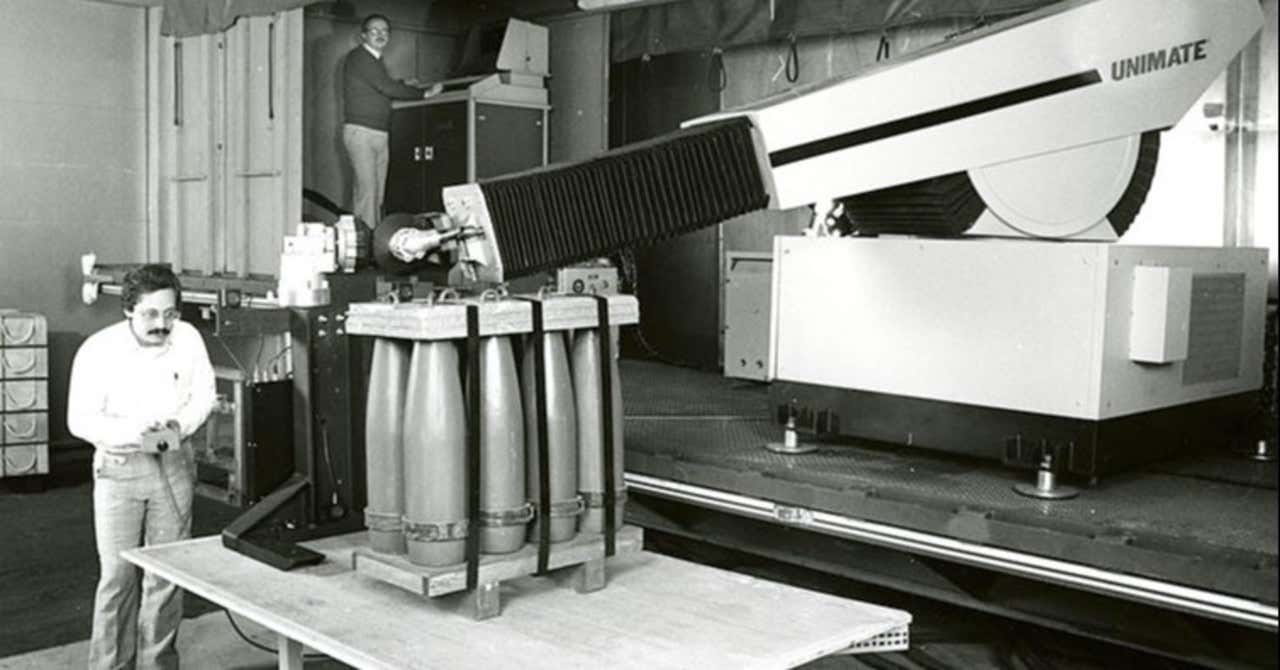
\includegraphics[width=8cm]{figs/unimate}
  \end{center}
  \caption{Robot Unimate.}
  \label{fig:unimate}
\end{figure}\




Con el avance de la informática en la segunda mitad del siglo XX, la robótica se integró cada vez más con la inteligencia artificial. Los robots dejaron de ser simples máquinas mecánicas para empezar a incorporar sensores y software que les permitían interactuar con su entorno de manera más flexible, como Shakey (Figura \ref{fig:shakey}), que podía tomar decisiones básicas sobre cómo moverse en su entorno.

\begin{figure} [H]
  \begin{center}
    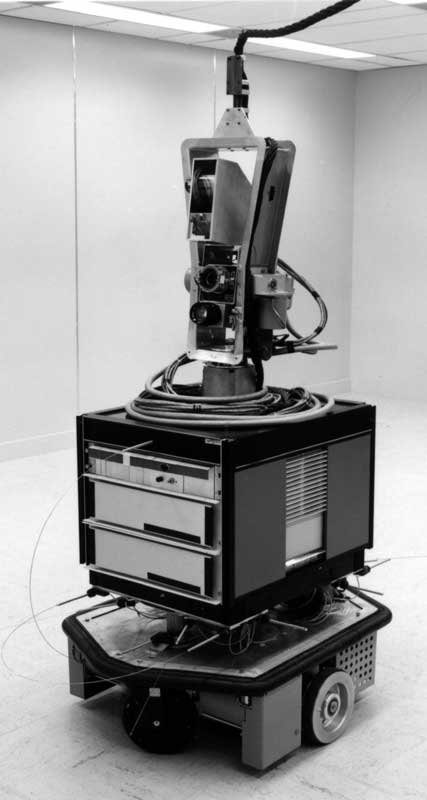
\includegraphics[scale=0.3]{figs/shakey}
  \end{center}
  \caption{Robot Shakey.}
  \label{fig:shakey}
\end{figure}\

En la actualidad se está aplicando en agricultura, logística, salud y exploración espacial, mostrando una evolución hacia máquinas más inteligentes, autónomas y adaptables. Hoy en día, los robots no solo ejecutan órdenes programadas, sino que también pueden aprender a partir de datos, tomar decisiones en tiempo real y adaptarse a entornos cambiantes. \\





\section{Robótica industrial}
\label{sec:segundaseccion}

La robótica industrial es el área de la robótica enfocada en el diseño, desarrollo y uso de robots en entornos industriales, cuyo objetivo es automatizar procesos productivos para mejorar la eficiencia, precisión, y seguridad en la fabricación de bienes. Los robots industriales son programables y están diseñados para realizar tareas repetitivas y a veces peligrosas para los humanos. Estos tipos de robots tienen alta precisión, velocidad y eficiencia y son versátiles. \\ \\ \\

\noindent\textbf{Manipuladores} 

Son un tipo de robot que se asemeja a un brazo humano y está diseñado para interactuar con su entorno a través de una serie de movimientos controlados. Estos robots están equipados con una serie de articulaciones que les permiten realizar tareas precisas y repetitivas, como agarrar, mover, ensamblar o manipular objetos. Suelen tener entre 3 y 7 grados de libertad que son las diferentes formas en las que el brazo puede moverse como rotaciones, desplazamientos lineales, etc. Un ejemplo de estos tipos son los robots Kuka\footnote{\url{https://www.kuka.com/es-es/productos-servicios/sistemas-de-robot/robot-industrial/kr-470-pa}} (Figura \ref{fig:kuka}) y los Yamaha\footnote{\url{https://global.yamaha-motor.com/business/robot/lineup/ykxg/large/}} (Figura \ref{fig:yamaha}).


\begin{figure}[h!]
  \begin{minipage}{0.48\textwidth}
    \centering
    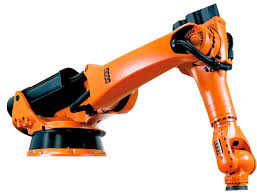
\includegraphics[width=6.5cm]{figs/kuka}
    \caption{Robot KUKA.}
    \label{fig:kuka}
  \end{minipage}
  \hfill
  \begin{minipage}{0.48\textwidth}
    \centering
    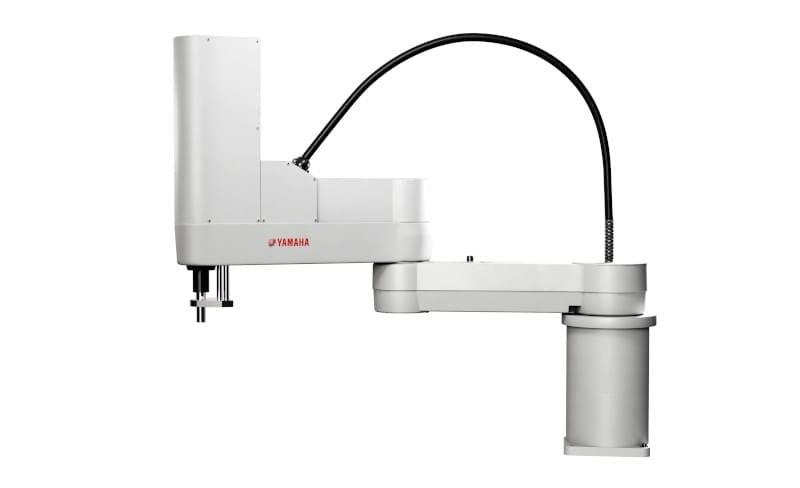
\includegraphics[width=8cm]{figs/yamaha}
    \caption{Robot Yamaha.} 
    \label{fig:yamaha}
  \end{minipage}
\end{figure}

\noindent\textbf{Cartesianos} 

Estos robots se mueven a lo largo de tres ejes lineales ortogonales (X, Y, Z), como el DL ROB2X-1200(Figura \ref{fig:cartesiano}), siguiendo el sistema de coordenadas cartesianas. Tiene una estructura sencilla y es adecuado para realizar movimientos precisos y repetitivos en trayectorias rectas. Se usan normalmente en tareas de pick and place o impresión 3D, entre otras.
 


\begin{figure} [h!]
  \begin{center}
    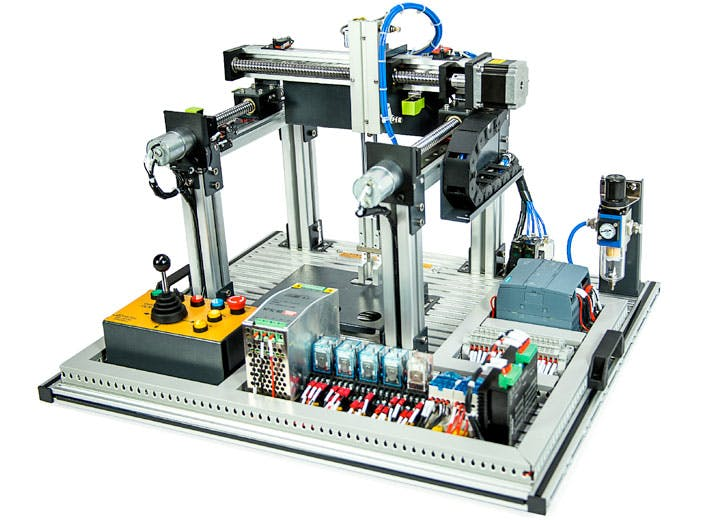
\includegraphics[width=6.5cm]{figs/cartesiano}
  \end{center}
  \caption{DL ROB2X-1200.}
  \label{fig:cartesiano}
\end{figure}\

\noindent\textbf{Delta} 




Se caracterizan por su diseño de brazos paralelos a la base y su capacidad para realizar movimientos rápidos y precisos en un espacio tridimensional, como por ejemplo el ABB IRB 360\footnote{\url{https://new.abb.com/products/robotics/robots/delta-robots/irb-360}} (Figura \ref{fig:delta}). Este tipo de robot se utiliza principalmente en aplicaciones de manipulación y ensamblaje debido a su alta velocidad y su capacidad para manejar objetos livianos con gran precisión. 

\begin{figure} [h!]
  \begin{center}
    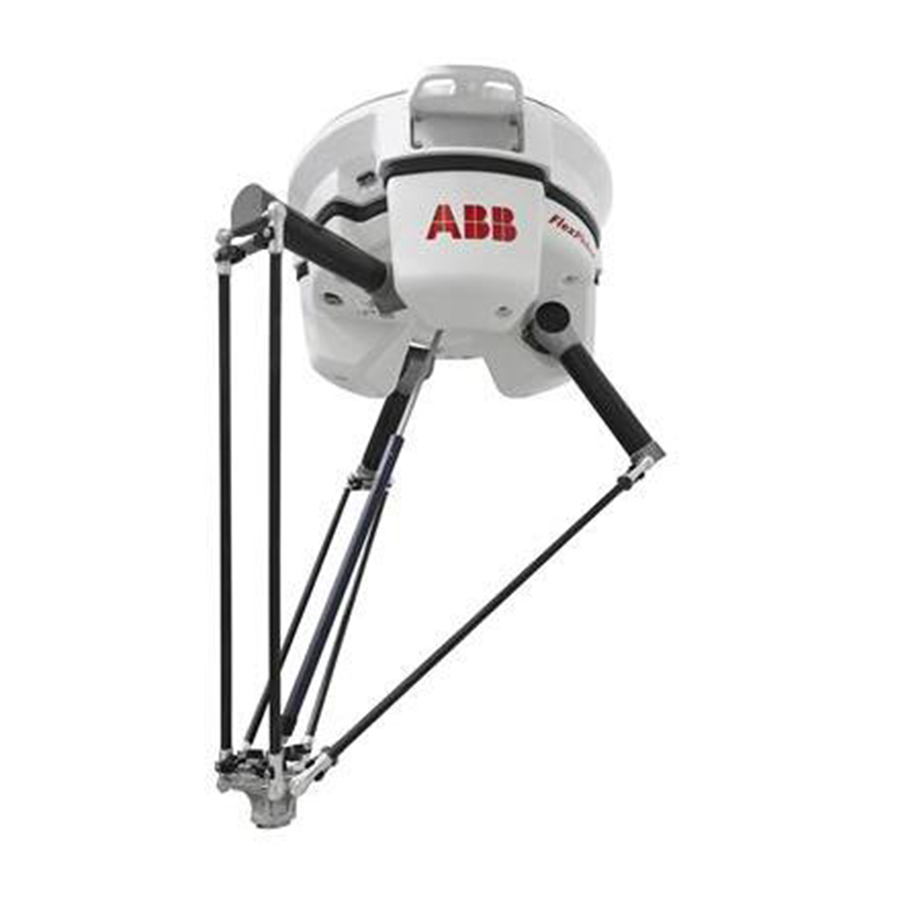
\includegraphics[width=8cm]{figs/delta}
  \end{center}
  \caption{ABB IRB 360.}
  \label{fig:delta}
\end{figure}\


La robótica es un campo que avanza rápidamente, con el objetivo de desarrollar máquinas inteligentes y autónomas capaces de llevar a cabo tareas cada vez más sofisticadas. Este progreso, liderado en gran medida por la robótica industrial, no solo impacta en los procesos productivos, sino que también aumenta la demanda de profesionales capacitados en este ámbito. Para satisfacer esta necesidad, la robótica educativa juega un papel crucial, permitiendo que las personas adquieran habilidades prácticas y conocimientos tecnológicos desde una etapa temprana. De esta forma, ambos enfoques se complementan para preparar a las nuevas generaciones para un entorno cada vez más automatizado. En la siguiente sección veremos en profundidad el alcance de la robótica educativa.


\section{Robótica educativa}
\label{sec:terceraseccion}


La robótica educativa se ha vuelto crucial en los últimos tiempos ya que prepara a las nuevas generaciones para un futuro tecnológico, fomentando habilidades clave en los institutos; como las matemáticas, la programación, la resolución de problemas y la electrónica, que es lo que se conoce como \hyperlink{STEM}{STEM} (Science, Technology, Engineering and Mathematics). También reduce brechas educativas y capacita a los estudiantes para enfrentar los retos de un mundo cada vez más automatizado.\\

La participación creciente de los robots móviles en nuestra vida cotidiana ha impulsado la creación de programas educativos que incorporan actividades prácticas de robótica en escuelas primarias y secundarias, promoviendo habilidades como la creatividad fomentando además el trabajo en equipo.\\


A principios de los 2000 algunas universidades y centros de formación empezaron a ofrecer cursos y talleres enfocados en la robótica educativa y se comenzaron a crear los primeros programas de robótica dirigidos a estudiantes, utilizando kits como LEGO Mindstorms (Figura \ref{fig:lego}), que facilitaban el aprendizaje de la programación y la construcción de robots.

\begin{figure} [h!]
  \begin{center}
    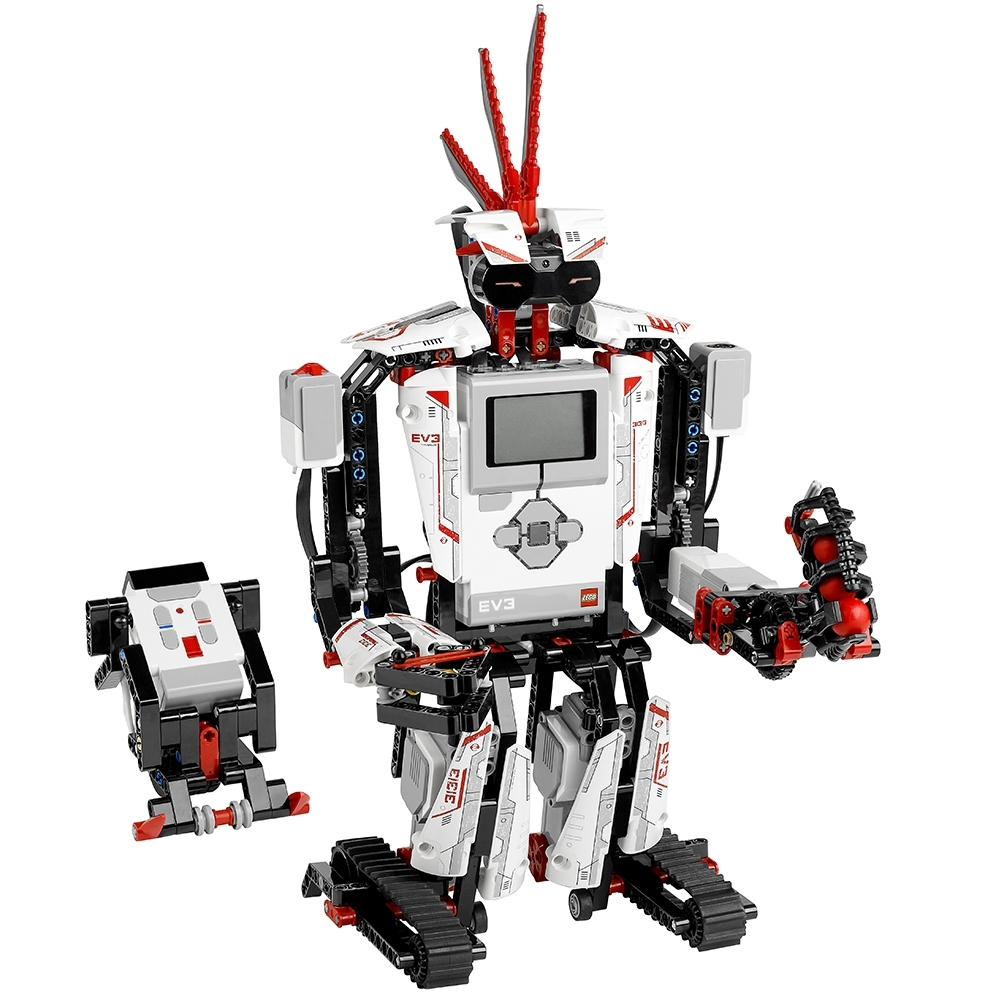
\includegraphics[width=8cm]{figs/lego}
  \end{center}
  \caption{LEGO MINDSTORMS EV3.}
  \label{fig:lego}
\end{figure}\



La creación de competiciones como la First Lego League \footnote{\url{https://firstlegoleague.soy/}} (Figura \ref{fig:First Lego League}) y la RoboCup Junior \footnote{\url{https://junior.robocup.org/}} (Figura \ref{fig:RoboCup Junior}), que llegaron a España a mediados de la década de 2010, dio un gran impulso a la robótica en las aulas y los estudiantes tuvieron la oportunidad de programar, diseñar y construir robots de distintos tipos para poder competir.



\begin{figure}[h!]
  \begin{minipage}{0.48\textwidth}
    \centering
    
\includegraphics[width=6.5cm]{figs/first-lego-league.jpg}
    \caption{First Lego League.}
    \label{fig:First Lego League}
  \end{minipage}
  \hfill
  \begin{minipage}{0.48\textwidth}
    \centering
    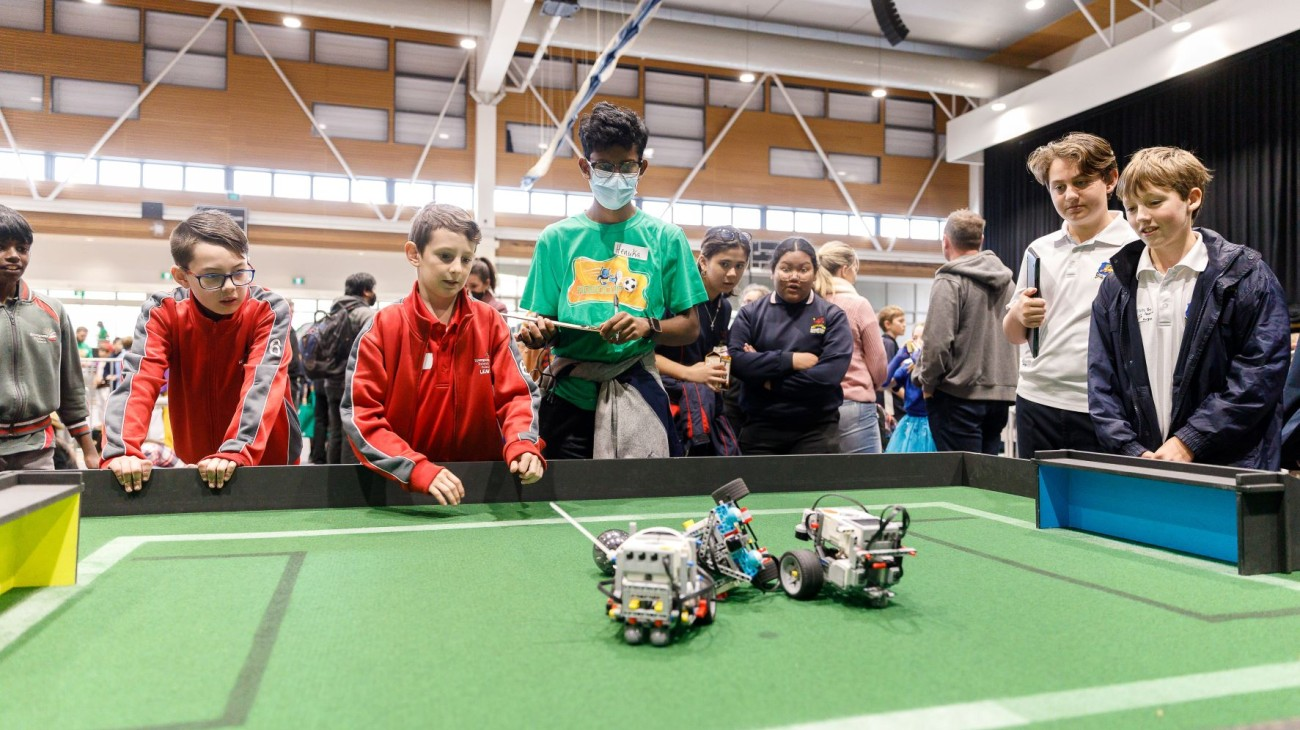
\includegraphics[width=8cm]{figs/RoboCup_junior.jpg}
    \caption{RoboCup Junior.} 
    \label{fig:RoboCup Junior}
  \end{minipage}
\end{figure}


Según el decreto \cite{Madrid}, se añadió la asignatura Tecnología, Programación y Robótica, en la cual los alumnos podrían estudiar los contenidos acerca de Scratch\footnote{\url{https://scratch.mit.edu/}} (Figura \ref{fig:scratch}) que utiliza bloques gráficos que los usuarios pueden arrastrar y soltar para crear programas, eliminando la necesidad de escribir código de texto y Arduino. 

\begin{figure} [h!]
  \begin{center}
    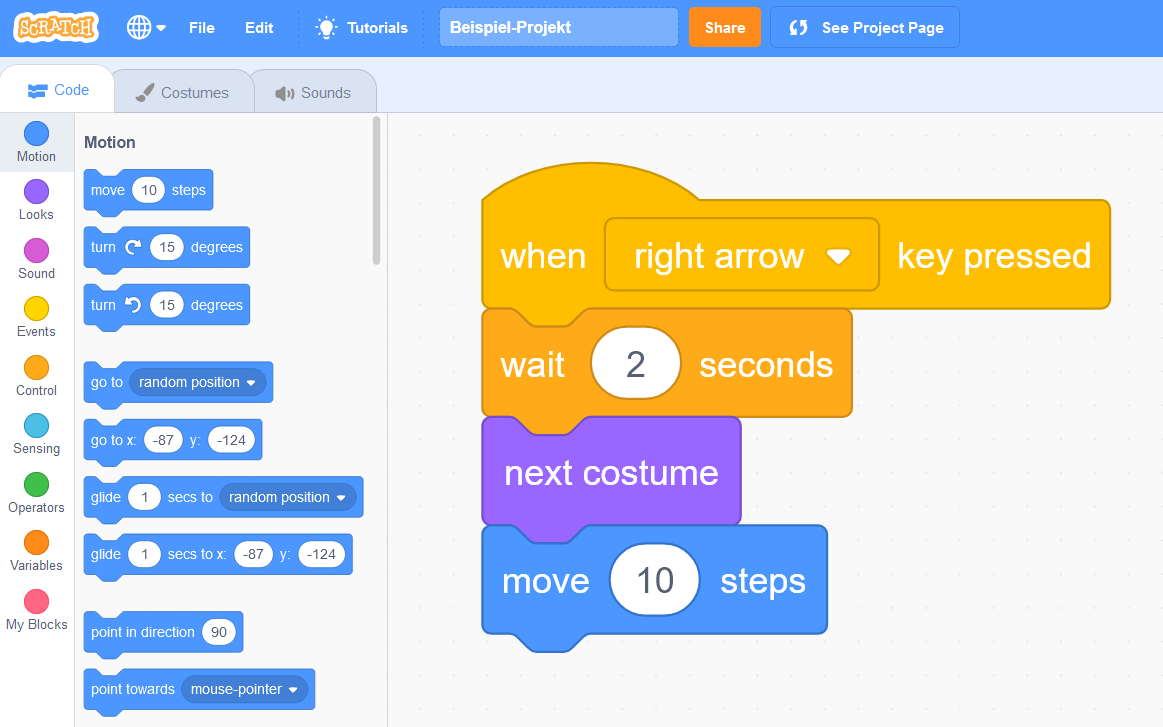
\includegraphics[width=8cm]{figs/scratch.png}
  \end{center}
  \caption{Programación con Scratch.}
  \label{fig:scratch}
\end{figure}\

Esta última tecnología debía de ser de bajo coste debido a la alta demanda y se usaron placas Arduino\footnote{\url{https://www.arduino.cc/}} (Figura \ref{fig:arduino}) y Raspberry Pi\footnote{\url{https://www.raspberrypi.com/}}(Figura \ref{fig:raspberry}), con las cuales se podían controlar sensores y actuadores de un robot de una manera más sencilla e interactiva para el usuario, aunque también tienen ciertas limitaciones a la hora de poder añadir algún hardware más complejo como un LIDAR para Arduino por ejemplo o algún actuador como motores con más potencia que requiera algún robot ya que en Raspberry, como mucho, se podrían controlar motores como las de las impresoras 3D, lo cual nos limita bastante a la hora de trabajar con robots de mayores dimensiones.


\begin{figure}[H]
  \begin{minipage}{0.48\textwidth}
    \centering
    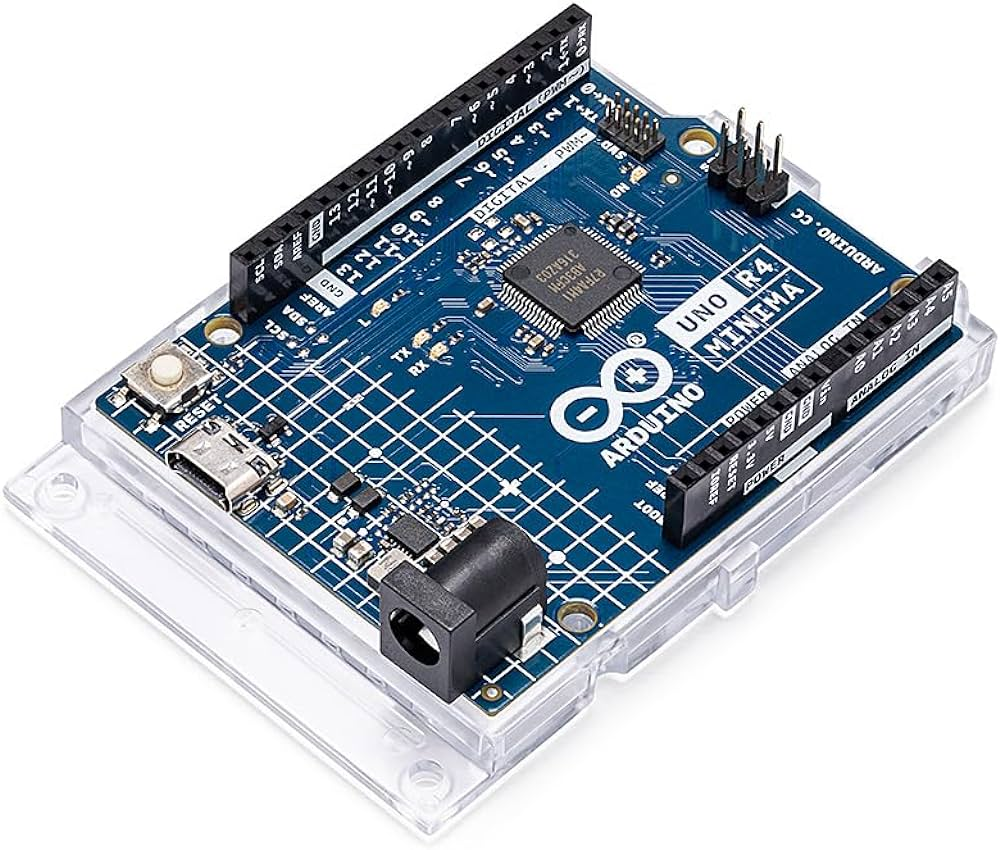
\includegraphics[width=6.5cm]{figs/arduino_uno.jpg}
    \caption{Arduino UNO.}
    \label{fig:arduino}
  \end{minipage}
  \hfill
  \begin{minipage}{0.48\textwidth}
    \centering
    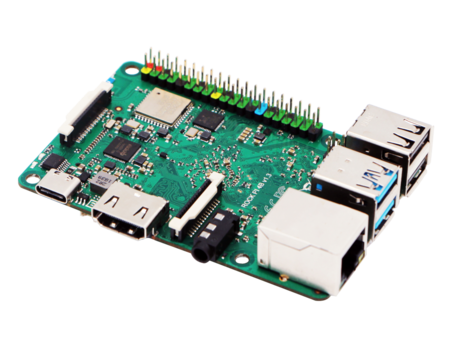
\includegraphics[width=7.2cm]{figs/raspberry4.png}
    \caption{Raspberry 4, Modelo B.} 
    \label{fig:raspberry}
  \end{minipage}
\end{figure}

Por eso se creó \hyperlink{ROS}{ROS} (Robot Operating System): un middleware estándar robótico que está estructurado como se indica en la Figura \ref{fig:ros}, para abordar varios desafíos y necesidades en la robótica moderna, especialmente en entornos de investigación y desarrollo de robots complejos cuyo propósito principal era proporcionar una infraestructura flexible y modular que permita a los desarrolladores e investigadores crear, integrar y controlar sistemas robóticos avanzados de manera más eficiente. El paso de \hyperlink{ROS}{ROS} a ROS2 fue un cambio necesario para abordar una serie de limitaciones y mejorar varios aspectos el soporte para sistemas en tiempo real, la seguridad y fiabilidad, soporte multiplataforma, etc.


\begin{figure} [h!]
  \begin{center}
    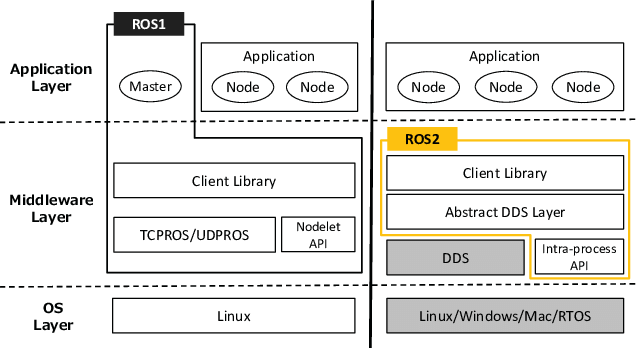
\includegraphics[width=10cm]{figs/ros.png}
  \end{center}
  \caption{Arquitectura de ROS y ROS2.}
  \label{fig:ros}
\end{figure}\

Con este middleware hay un salto muy grande en términos de aprendizaje ya que no es suficiente con conocer el lenguaje de programación sino que hay que entender todo el entorno de esta plataforma(estructuras de datos, programación modular, comunicaciones...), por lo que sería necesaria una conexión entre estos niveles de aprendizaje como por ejemplo alguna asignatura más o algún programa en la etapa de Bachillerato o Secundaria enfocada en este aspecto.\\

A medida que la robótica educativa ha evolucionado, los progresos en inteligencia artificial han abierto nuevas oportunidades para mejorar las capacidades y la autonomía de los robots. En este sentido, el aprendizaje automático ha comenzado a desempeñar un papel fundamental, permitiendo así que los robots no sigan solo instrucciones preprogramadas, sino que también aprendan de su entorno, optimicen su comportamiento y tomen decisiones basadas en datos. Esta combinación de robótica y aprendizaje automático no solo amplía el alcance de la educación \hyperlink{STEM}{STEM}, sino que también introduce a los estudiantes en conceptos clave de la inteligencia artificial, allanando el camino para sistemas más autónomos y sofisticados.


\section{Machine learning}


Dentro de la inteligencia artificial, se encuentra el ámbito del aprendizaje automático o Machine Learning. Un modelo de aprendizaje automático consiste en un archivo inteligente que se ha condicionado con un algoritmo para poder aprender patrones específicos en diferentes conjuntos de datos y así proporcionar información y predicciones a partir de ellos.\\

Al crear un modelo de aprendizaje automático, se define la respuesta que se desea capturar y se establecen los parámetros con los que debe funcionar y de los que debe aprender el modelo. Cuando se habilita un modelo de aprendizaje automático a través de un algoritmo, este puede empezar aprendiendo el conjunto de datos y descubriendo la información. Cuanta más información obtiene el modelo, más puede utilizar el conocimiento para acelerar y mejorar el descubrimiento.\\ 

Aunque los ordenadores no cuentan con la capacidad de razonar y aprender con la experiencia, los algoritmos que alimentan estos modelos funcionan para simular esa experiencia en la medida de lo posible. Con los parámetros y ajustes de los algoritmos, los modelos pueden replicar el aprendizaje de la experiencia y eso facilita un profundo nivel de análisis y predicciones que resultarían imposibles de otro modo. \\

El algoritmo que emplean para aprender se ha creado utilizando datos de entrenamiento y de prueba, y genera una estimación en los datos partiendo de un patrón. Estos datos pueden estar etiquetados o no; y, si lo están, quiere decir que el modelo lo debe identificar en su justa medida. Después, la función de error evaluará la precisión del modelo sobre la decisión que ha tomado y se observará cuánto de preciso es el modelo sobre esos datos. Por último, se optimizarán los modelos en la medida de lo posible ajustando los diferentes parámetros para que se pueda adaptar mejor al conjunto de datos de entrenamiento hasta poder cumplir un umbral de precisión.\\ 



Existen diferentes tipos de aprendizaje en Machine Learning: 

\begin{itemize}
 \item \textit{Aprendizaje supervisado.} En este método, los conjuntos de datos están etiquetados y se conoce la salida y el modelo se entrena con los datos de la salida conocida; es decir, para entrenar el al algoritmo para que reconozca fotos de manzanas, hay que transmitirle fotos etiquetadas como manzanas (regresión lineal, árboles de decisión, etc.).
 \item \textit{Aprendizaje no supervisado.} Es un modelo que usa datos sin etiquetar con el objetivo de aprender patrones y no cuenta con un conjunto entrenado previamente. El algoritmo en este caso aprende de los datos sin intervención humana y los categoriza en grupos según los atributos, por lo que es bueno para la coincidencia de patrones (mínimos cuadrados, K-means, etc.).
 \item \textit{Aprendizaje semisupervisado.} En este modelo, solo se etiquetan algunos datos y el algoritmo debe determinar cómo organizar y estructurar los datos para lograr un resultado conocido. Por ejemplo, al modelo de aprendizaje automático se le dice que el resultado es una pera, pero solo algunos datos de entrenamiento están etiquetados como una pera.
\end{itemize}\

El aprendizaje automático ha impulsado avances importantes en la autonomía y la capacidad de decisión de los robots, lo cual ha facilitado la creación de sistemas más inteligentes y adaptativos. Sin embargo, la implementación de estas tecnologías a menudo se ve limitada por los altos costos del hardware y la infraestructura computacional necesarios para entrenar y ejecutar modelos complejos. En este contexto, la robótica de bajo costo se presenta como una alternativa para tener acceso a estas innovaciones, permitiendo así que investigadores, educadores y entusiastas experimenten con inteligencia artificial sin requerir grandes inversiones. Gracias al uso de componentes asequibles y plataformas de código abierto, es posible integrar algoritmos de aprendizaje automático en sistemas robóticos económicos, ampliando su uso en educación, investigación y desarrollo.

 
\label{sec:cuartaseccion}


\section{Robótica de bajo coste}
\label{sec:quintaseccion}

La robótica de bajo coste está enfocada en el diseño, desarrollo y uso de sistemas robóticos que son accesibles económicamente, usando componentes de bajo coste pero sin eliminar la funcionalidad básica con el objetivo de reducir la complejidad de los sistemas ya existentes. Esto ha tenido un gran impacto en áreas como la educación y la investigación académica.\\

El uso de la impresión 3D y el software libre, junto con el uso de componentes económicos, ha dado paso a la creatividad de los usuarios para crear piezas con un propósito específico personalizadas a un precio más asequible que si las hubieran tenido que comprar ya hechas.\\


Todo esto ha fomentado la filosofía \hyperlink{DIY}{DIY}, que promueve la personalización y creación propia de objetos y proyectos de forma autónoma. Todo esto sin tener que depender de productos comerciales ya construidos previamente.\\

Un ejemplo de esta área es el robot Makeblock mBot\footnote{\url{https://www.makeblock.com/pages/mbot-robot-kit}} (Figura \ref{fig:mbot-2}) desarrollado por la empresa china Makeblock, que se usaba en las escuelas para enseñar programación y electrónica y era compatible con muchos sensores y accesorios, además de poder usar microcontroladores como el de Arduino, por lo que era ideal para aportar soluciones creativas en este ámbito.

\begin{figure} [H]
  \begin{center}
    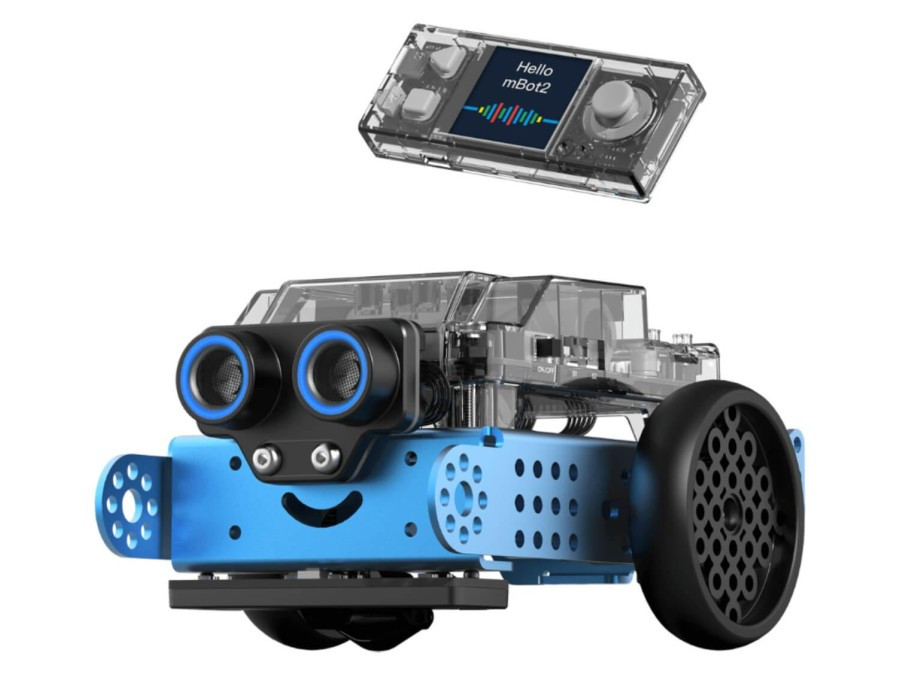
\includegraphics[width=6cm]{figs/mbot-2.jpg}
  \end{center}
  \caption{Makeblock mBot.}
  \label{fig:mbot-2}
\end{figure}\


Otro ejemplo de robot de bajo coste ampliamente usado en educación es el TurtleBot\footnote{\url{https://www.turtlebot.com/turtlebot3/}} (Figura \ref{fig:turtlebot}). Este fue desarrollado por la empresa Willow Garage, los creadores de \hyperlink{ROS}{ROS}, y el objetivo era ofrecer una plataforma robótica económica y accesible. Por ello, las universidades empezaron a usarlo, ya que las instituciones educativas enfrentaban problemas en cuanto al presupuesto, por lo que este robot era el ideal para poder experimentar con \hyperlink{ROS}{ROS} de una manera más asequible para los estudiantes, ya que el presupuesto era relativamente barato en comparación con otras plataformas robóticas que había en el momento.

\begin{figure} [H]
  \begin{center}
    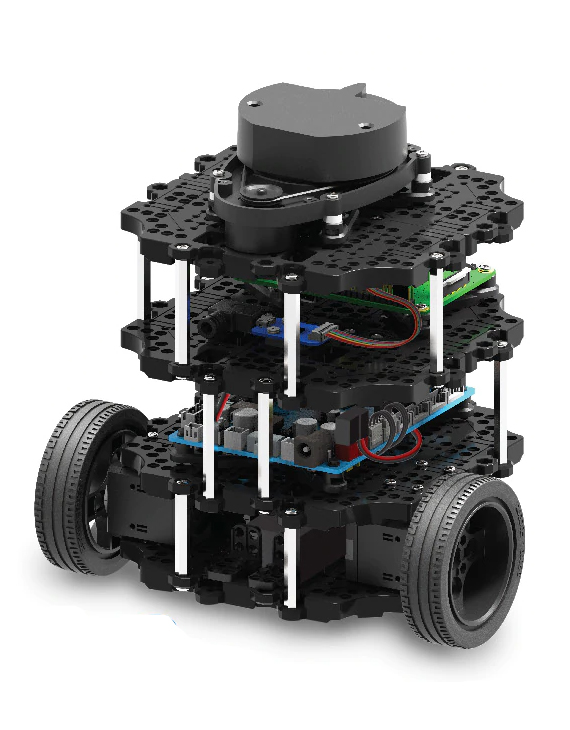
\includegraphics[scale=0.25]{figs/turtlebot3burguer.jpg}
  \end{center}
  \caption{TurtleBot 3 Burger.}
  \label{fig:turtlebot}
\end{figure}\


El presente trabajo está enfocado en la fabricación y programación de un robot móvil de bajo coste diseñado para que sea fácil de usar a partir de diferentes componentes hardware y piezas diseñadas en 3D, siguiendo así la filosofía \hyperlink{DIY}{DIY}. Mediante diferentes técnicas y procedimientos, como los modelos de aprendizaje automáticos, se podrá obtener una estimación precisa de cuántos dispositivos de red son necesarios para que el robot pueda localizarse en interiores de la mejor manera posible y a partir de una interfaz \hyperlink{HRI}{HRI} amena, se podrá controlar al robot por comandos de voz mediante técnicas avanzadas. Finalmente, se presentarán diferentes métodos para que el robot pueda navegar por diferentes trayectorias siguiendo un camino hacia un objetivo claro a partir de los comandos de voz y para que sea portable a diferentes entornos de la manera más asequible posible. Uno de los objetivos es lograr que funcionen todos estos métodos y procedimientos en una CPU de baja capacidad de cómputo, como la Raspberry, y que sea portable a diferentes entornos en interiores de la manera más asequible posible. En el siguiente capítulo se presentarán diferentes investigaciones y estudios previos que tienen una cierta similitud con el diseño y la programación interna del robot que se ha fabricado.

\vspace{15cm} % Espacio vertical de 1 cm









\chapter{Estado del arte}
\label{cap:capitulo2}
\setcounter{page}{1}

\begin{flushright}
\begin{minipage}[]{10cm}
\emph{Eres el amo de tu destino, el capitán de tu alma.}\\
\end{minipage}\\

Napoleon Hill, \textit{Piense y hágase rico}\\
\end{flushright}

\vspace{1cm}

En este capítulo se definirán algunos de los trabajos que han tenido más importancia en este proyecto.\\

En \cite{9815716}, se presentan diferentes alternativas sobre cómo controlar motores de corriente continua mediante señales PWM a los microcircuitos o en este caso motores reductores mediante un módulo controlador de motor L298N puede regular la velocidad y la dirección an ambos sentidos de los motores al mismo tiempo, lo cual es muy importante ya que de esta manera no haría falta sincronizar ambos motores de ninguna manera.\\

Por otra parte, se necesitará averiguar qué modelo de aprendizaje automático(Figura \ref{fig:random_forest}) es el ideal para poder clasificar correctamente comandos por voz en diferentes clases. Esto se presenta en \cite{Zenkov-sklearn-SER-basics}, en el cual se ofrecen diferentes técnicas que se pueden aplicar a problemas de clasificación, de regresión y técnicas de ingeniería de características para datos de audio y un vistazo en profundidad a la lógica, conceptos y propiedades de las redes neuronales profundas actuales. También se proporciona información sobre algunos modelos clave de aprendizaje automático y la lógica en la elección de sus hiperparámetros, cuyos objetivos están enmarcados por la tarea de reconocer comandos de audio por voz.\\

\begin{figure} [H]
  \begin{center}
    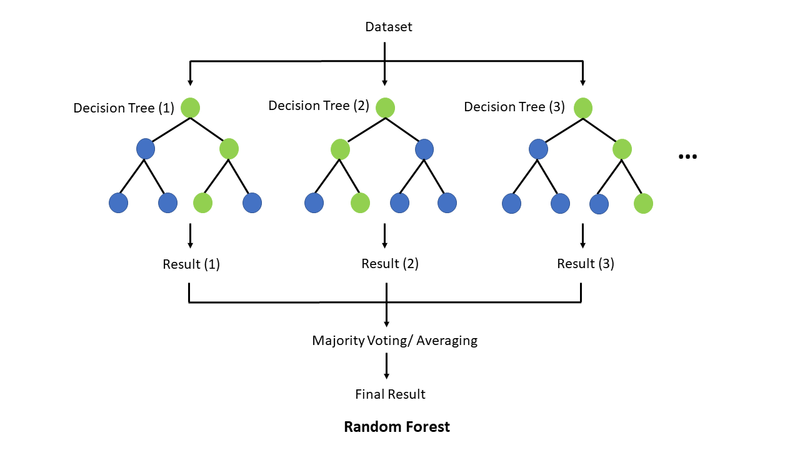
\includegraphics[scale=0.8]{figs/random_forest}
  \end{center}
  \caption{Algoritmo de aprendizaje automático Random forest.}
  \label{fig:random_forest}
\end{figure}\

En este otro artículo \cite{unknown}, se realiza un estudio sobre los sistemas de posicionamiento en interiores de "fingerprinting"(Figura \ref{fig:wifi}) que utiliza modelos de aprendizaje automático para crear un mapa de ubicación RSSI del entorno para una mejor estimación de la ubicación y que a diferencia de los sistemas de posicionamiento en interiores \hyperlink{BLE}{BLE} que se han implementado con modelos de pérdida de propagación, los cuales han demostrado estimar posiciones con grandes errores debido a la incertidumbre de las señales RSSI causadas por obstáculos interiores y fenómenos electromagnéticos, los de fingerprinting consiguen una mejor estimación de la posición. Para demostrarlo, se probarán diferentes hipótesis como las siguientes:

\begin{enumerate}
 \item ¿La precisión de las balizas 
\hyperlink{BLE}{BLE} escala linealmente con la cantidad de las mismas?
 \item ¿La precisión aumenta
cuando la distancia mínima entre dos posiciones es de 1 m mientras que el área de mapeo no cambia?
\end{enumerate}\ 

\begin{figure} [H]
  \begin{center}
    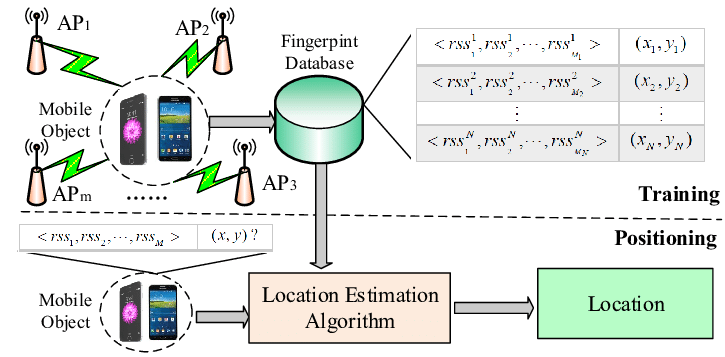
\includegraphics[scale=0.6]{figs/wifi}
  \end{center}
  \caption{Principio de WiFi fingerprinting.}
  \label{fig:wifi}
\end{figure}\

Los resultados de ambas hipótesis fueron verdaderas, por lo que para este proyecto servirá de gran ayuda para saber con precisión cuántos puntos de acceso WiFi son necesarios para un entorno. En este caso no se usarán balizas Bluetooth pero el procedimiento sería el mismo. Para poder estimar la posición del robot en el mapa mediante balizas WiFi, se hará uso de la trilateración(Figura \ref{fig:trilateration}), la cual es una técnica presentada y estudiada en este artículo \cite{inproceedings}, el cual presenta un método basado en WiFi para el posicionamiento en interiores utilizando
mediciones de intensidad de señal recibida (RSS). También se estiman las distancias entre los puntos de acceso (\hyperlink{APs}{APs}) y el dispositivo móvil a partir de
valores RSS evaluados por el modelo de propagación de la señal. Esto servirá a calcular mediante diferentes fórmulas la posición del robot en el mapa conociendo a su vez la posición de las balizas y ver cuánto error hay en la estimación.\\


\begin{figure} [H]
  \begin{center}
    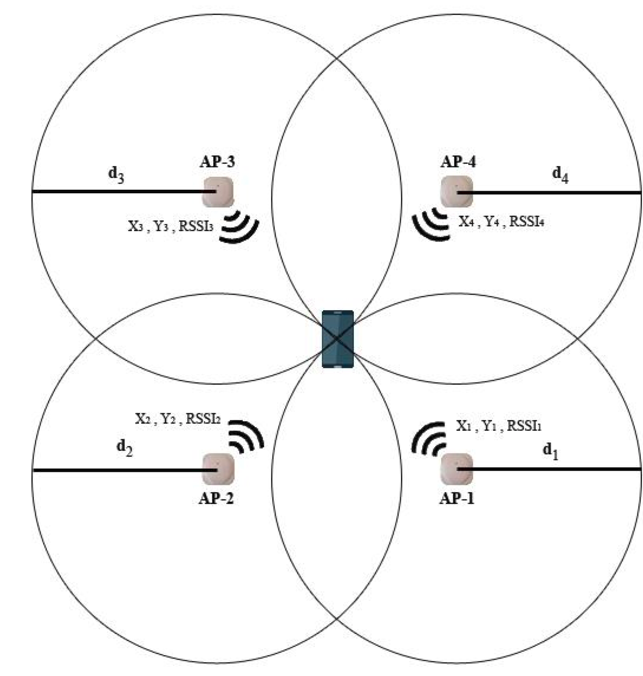
\includegraphics[scale=0.4]{figs/trilateration}
  \end{center}
  \caption{Técnica de trilateración por WiFi.}
  \label{fig:trilateration}
\end{figure}\

A su vez, es importante entender las aplicaciones de los algoritmos de planificación de rutas. Para ello, este artículo \cite{article} sirve como introducción al concepto de planificación de rutas y navegación en el contexto de la robótica, y a los algoritmos y los casos de uso donde los nuevos especialistas en robótica pueden desarrollar aplicaciones de
búsqueda o planificación de rutas para satisfacer sus necesidades educativas en este contexto. También se realiza un estudio el algoritmo de búsqueda A* (Figura \ref{fig:astar}) y sus aplicaciones para un sistema de navegación para vehículos robóticos, el cual es que se usará en este trabajo debido a que encaja perfectamente en cuanto a la optimización, la precisión y el tiempo de ejecución.

\begin{figure} [H]
  \begin{center}
    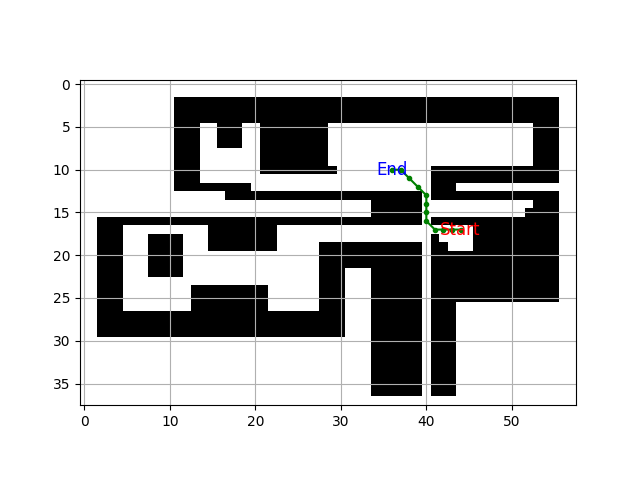
\includegraphics[scale=0.4]{figs/astar}
  \end{center}
  \caption{Algoritmo de búsqueda A*.}
  \label{fig:astar}
\end{figure}\

Una vez se ha entendido el concepto de planificación de rutas el robot debe saber como desplazarse por la misma, siendo capaz ya de desplazarse en línea recta y de localizarse pero se tienen en cuenta los giros que debe hacer en la ruta, por lo que se hará uso de un magnetómetro para cononcer el ángulo de orientación del robot y así hacer giros más precisos. Otro paso importante como se puede apreciar en este documento \cite{Ozyagcilar2015} son las diferentes técnicas para la calibración del sensor, en el cual se proporciona la teoría para la calibración de una brújula electrónica de un teléfono inteligente para mitigar los efectos de hard y soft-iron, los cuales son los efectos producidos por materiales ferromagnéticos y que pueden magnetizarse sobre el magnetómetro.

También habría que entender el filtro de paso bajo como se explica en este otro artículo \cite{low_pass_filter}, el cual es fácil de implementar, utiliza muy pocos recursos y, con dos parámetros fáciles de entender como ya se explicará más adelante, es fácil de ajustar, ya que en comparación con otros filtros,
tiene menos desfase.



\vspace{15cm} % Espacio vertical de 1 cm









\chapter{Objetivos}
\label{cap:capitulo3}

\begin{flushright}
\begin{minipage}[]{10cm}
\emph{La proactividad es la clave para el éxito}\\
\end{minipage}\\

Stephen R. Covey, \textit{Los 7 hábitos de la gente altamente efectiva}\\
\end{flushright}

\vspace{1cm}

Una vez revisado el estado del arte correspondiente a este trabajo, se presenta el plan de trabajo de este, definiendo los 
objetivos que se han marcado, tanto específicos como generales, para poder desarrollar este proyecto, y los requisitos necesarios para el mismo.
Finalmente, se explica la metodología que se ha seguido para poder cumplir los objetivos propuestos.



\section{Descripción del problema}
\label{sec:descripcion}


El objetivo general de este proyecto es el desarrollo y diseño de un prototipo de robot guía de bajo coste, con el fin de ofrecer una solución más accesible y asequible frente a los robots guía convencionales, los cuales son generalmente caros y difíciles de adaptar a diferentes entornos debido a todos los cambios que serían necesarios a nivel de software. El sistema se diseñará para maximizar la eficiencia con los recursos disponibles, garantizando un equilibrio entre coste y funcionalidad. Esto llevará a soluciones innovadoras en el diseño del hardware y la optimización del software, permitiendo que el robot sea viable sin necesidad de componentes de alto coste. Este robot, mediante una interfaz \hyperlink{HRI}{HRI} amigable, usará comandos de voz para poder comunicarte con él para guiar a las personas en espacios interiores. A diferencia de las soluciones existentes, que utilizan materiales costosos y sensores avanzados, este prototipo utilizará una CPU de baja capacidad de cómputo, como la Raspberry Pi, y técnicas avanzadas de localización interna  junto con algoritmos de navegación. Asimismo, se busca que el sistema creado sea portable para la mayoría de entornos en interiores de la manera más asequible posible sin necesidad de tener una complejidad mayor en otros entornos a la hora de programarlo y que sea capaz de poder orientarse y localizarse en el mapa mediante diferentes sensores y actuadores hasta llevar a la persona a un punto en concreto. Esto proporciona una opción más económica, práctica y versátil para la navegación en interiores.\\ 

Para cumplir con el objetivo general establecido, será necesario establecer los siguientes objetivos específicos:


\begin{enumerate}
 \item Explorar diferentes opciones de diseño para determinar la forma final del robot.
 \item Realizar una investigación sobre los distintos componentes tanto hardware como software que hay disponibles en el mercado que sean 
de bajo coste y que satisfagan las tareas de localización y movimiento del robot.
 \item Desarrollar el software necesario para poder gestionar el control del prototipo desde el ordenador sin necesidad de cables intermedios.
 \item Uso de \hyperlink{CAD}{CAD} (Computer-Aided Design) para el diseño de piezas 3D mediante el uso de software libre, como FreeCAD.
 \item Hacer uso de una impresora 3D para poder materializar las piezas necesarias. 
 \item Poder combinar todos los datos de navegación y localización sin que intervengan unos con otros mediante la librería threading que permite el control y la ejecución de diferentes hilos ejecutados en paralelo.
 \item Realizar la calibración necesaria de los sensores para asegurar la precisión de las lecturas y que sea fiable.
 \item Entrenar una red neuronal con diferentes audios por voz para enseñar a la red a clasificar e interpretar las órdenes dadas por el usuario para
 que te guíe a un sitio específico dependiendo de la orden dada por voz.
\end{enumerate}\


\section{Requisitos}
\label{sec:requisitos}

Con el objetivo de solucionar los problemas descritos, se han establecido los siguientes requisitos:

\begin{itemize}
 \item \textit{} El sistema propuesto deberá de ser capaz de poder ejecutarse en tiempo real en la plataforma Raspberry Pi 4B.
 \item \textit{} Python será el lenguaje de programación usado porque es fácil de usar, a parte de contar con una amplia gama de bibliotecas 
 y librerías útiles para este proyecto y tener soporte completo en el sistema operativo de la Raspberry Pi 4B.
 \item \textit{} El diseño y la fabricación de este prototipo no debe suponer un coste mayor a 145 \euro.
 \item \textit{} Las piezas que se usen para el diseño del robot deben ser imprimibles en cualquier impresora 3D actual.
 \item \textit{} Debe ser capaz de desplazarse sin problemas por la mayoría de suelos que hay en entornos interiores.
 \item \textit{} Es necesario que esté fabricado con el menor número de piezas posibles en 3D debido a alto tiempo que tardan en imprimirse algunas
 con el objetivo de que el usuario lo pueda montar en poco tiempo.
 \item \textit{} Contar con varios \hyperlink{APs}{APs} para que el robot se pueda localizar, por lo que mínimo con 3 valdría aunque depende de las interferencias que haya en los distintos entornos puede que se necesiten más.
 \item \textit{} Los motores y la batería deben de pesar lo menos posible, ya que a parte irán incorporadas la Power Bank y la Raspberry encima y a su vez deben proporcionar la potencia necesaria para mover todo el hardware sin problemas.
 \item \textit{} La batería debe ser recargable para que pueda usarse el robot todas las veces que se quiera y que dure lo máximo posible.
 
\end{itemize}\

 
\section{Metodología}
\label{sec:metodologia}

Con el fin de alcanzar los objetivos propuestos, se han utilizado distintas herramientas para poder desarrollar el proyecto correctamente y
hacer un control y seguimiento del mismo.\\

A través de la aplicación Microsoft Teams se han organizado tutorías semanales con el tutor del trabajo para hacer un seguimiento del proyecto. En estas reuniones se comentaban los problemas que iban surgiendo a lo largo de la semana y las posibles soluciones que se podían tomar para avanzar correctamente, además de la evaluación y el control de los objetivos que se habían marcado la semana anterior y establecer los nuevos objetivos y planteamientos de cara a la siguiente semana. También se ha utilizado el correo electrónico para comentar con el tutor las dudas y problemas que iban surgiendo a lo largo de la semana.\\ 

Para mantener el código y exponer los avances de este proyecto, se ha usado un repositorio de GitHub\footnote{\url{https://github.com/RoboticsURJC/tfg-vdelatorre}}, en el cual se ha ido subiendo todo el código necesario y los diferentes recursos empleados, así como imágenes, piezas, audios, artículos, etc. Al mismo tiempo, se ha diseñado una Wiki\footnote{\url{https://github.com/RoboticsURJC/tfg-vdelatorre/wiki}} en el mismo repositorio que incluye todo el proceso que se ha ido siguiendo paso a paso, junto con los diferentes problemas que han ido surgiendo y las soluciones empleadas, e imágenes y vídeos para demostrar todos los experimentos realizados y el comportamiento final del prototipo.

\section{Plan de trabajo}
\label{sec:plantrabajo}

El desarrollo completo de este proyecto se ha dividido en las siguientes etapas:

\begin{enumerate}
 \item \textit{Investigación del hardware utilizado.} El periodo de septiembre a octubre de 2023, se dedicó al aprendizaje del funcionamiento de los diferentes sensores, para poder trabajar con la Raspberry a través de comandos por voz y una red neuronal entrenada para ello.

 \item \textit{Investigación del estado del arte.} En el periodo de octubre a noviembre de 2023, se hizo una investigación en diferentes plataformas, como Google Scholar, sobre artículos relacionados con el funcionamiento de la idea descrita y la compatibilidad y si era viable o no el proyecto.
 
  \item \textit{Ampliación del dataset.} En el periodo de noviembre a enero se estuvo ampliando el dataset de audios con diferentes voces y comandos para ver si era viable a largo plazo y si era escalable o no, para comprobar si era compatible con diferentes tipos de voces.
  
  \item \textit{Pruebas con motores.} En el periodo de diciembre hasta abril, se estuvo probando y analizando los motores más potentes, de menor coste y de menor peso de los que se disponía, y al mismo tiempo se estuvo diseñando las piezas para anclarlas robot y pensando en la estructura final para poder combinar todos los componentes. Estas piezas, una vez fueron diseñadas por ordenador en FreeCAD\footnote{\url{https://www.freecad.org/index.php?lang=es_ES}}, fueron impresas en 3D haciendo uso de una impresora de filamento de tipo \hyperlink{FDM}{FDM} (Fused Deposition Modeling) y probadas una a una para ver si eran compatibles con los motores y disponían de la sujeción necesaria para que el robot pudiera desplazarse correctamente.
  
 \item \textit{Desarrollo de software.} Una vez montado el robot, en el periodo de abril hasta junio, se trasladó toda la red neuronal y el modelo del software probado ya con éxito en un sistema operativo Ubuntu a una Raspberry Pi probando las diferentes versiones, paquetes y librerías para que todo funcionase correctamente y se realizó una investigación acerca de qué modelo de Raspberry usar para soportar todo el cómputo necesario.
 
  \item \textit{Conexión VPN Raspberry Pi.} Para poder controlar el robot de manera independiente, en el periodo de junio hasta julio, se probó y se configuró el programa VNC Server en la Raspberry para no necesitar cables de conexión y el robot se pudiera mover libremente mientras es programado desde el ordenador.
  
 \item \textit{Navegación.} Para poder controlar el robot de manera independiente, en el periodo de julio hasta diciembre, una vez diseñado el robot y probado con ambos motores, se hizo una investigación acerca de la navegación y los posibles algoritmos necesarios para trazar la ruta óptima de un punto a otro. Por otra parte, se usó la herramienta de software libre \hyperlink{GIMP}{GIMP} para diseñar el mapa del robot en el que este va a navegar y también se exploraron las diferentes técnicas de navegación y localización.
 
   \item \textit{Pruebas del software desarrollado y escritura de la memoria.} En el periodo de enero hasta marzo de 2025, se realizaron todas las pruebas y cambios necesarios para que el robot cumpliera el objetivo y al mismo tiempo se fue elaborando el presente documento.
\end{enumerate}\



\chapter{Plataforma de desarrollo}
\label{cap:capitulo4}


\begin{flushright}
\begin{minipage}[]{10cm}
\emph{Cuando quieres algo, todo el universo conspira para que realices tu deseo}\\
\end{minipage}\\

Paulo Coelho, \textit{El Alquimista}\\
\end{flushright}

\vspace{1cm}

En este capítulo, se explicará con detalle todas las herramientas tanto a nivel hardware como software que han sido utilizadas para poder desarrollar el proyecto.


\section{Hardware}
\label{sec:hardware}

En esta sección se descibirán todos los componentes físicos que han sido utilizados en este trabajo, los cuales han sido adquiridos en su mayor parte por el precio y la funcionalidad que tienen.\\ \\
A continuación se explicará con detalle aquellos que están presentes en esta arquitectura hardware.

\subsection{Micrófono micro USB}
\label{subsec:micro}

Se trata de un tipo de micrófono(Figura \ref{fig:microfono-usb}), el cual es utilizado para la grabación de audio compatible con puertos USB y teniendo un pequeño tamaño y peso lo cual lo hace ideal para incorporarlo en la Raspberry. 


Se llegó a la conclusión de que era la mejor idea usar este tipo de micrófono, ya que no necesita clabes por lo que facilita al usuario comunicarse con el dispositivo siendo más cómodo para él. Además de ser bajo coste, tiene un precio que ronda los 10 \euro, es fácil de adquirir en páginas web como Amazon. Este tipo de micrófono tiene 2 metros de distancia efectiva y filtra el ruido de fondo no deseado, haciendo que el sonido sea más claro y limpio.


\begin{figure}[H] % Usa [H] para forzar la posición
  \begin{center}
    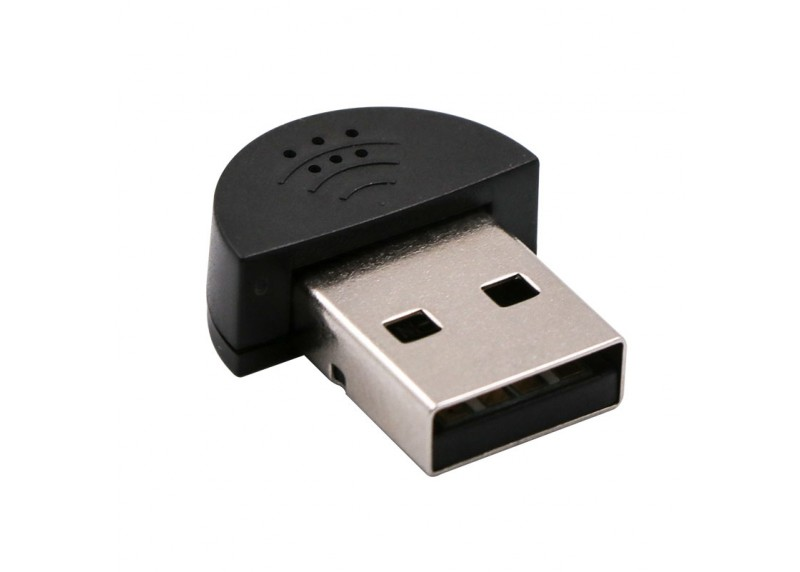
\includegraphics[scale=0.3]{figs/microfono-usb}
  \end{center}
  \caption{Micrófono micro USB.}
  \label{fig:microfono-usb}
\end{figure}


\subsection{Controlador driver L298N}
\label{subsec:l298n}

Un controlador de motor o driver(Figura \ref{fig:l298n}) sirve para controlar motores de corriente continua(DC) o motores paso a paso el cual, permite sobre todo controlar tanto la velocidad como la dirección de estos motores. Este módulo hardware tiene la capacidad de transformar las señales lógicas las cuales les envía el procesador a una serie de pulsos de potencia que alimentarán ambas bobinas de cada motor reductor para hacer girar cada uno de ellos en un orden concreto. A parte, dispone de protecciones para que no se dañe en el caso de que se haga un mal uso del mismo, y siendo su precio original por solo 3 \euro.\\ 

El control del mismo es simple, primero habría que conectar el positivo de la fuente de alimentación externa de 6 V a los 12 V de la placa(Vin), y teniendo el jumper de selección de 5 V activo, ya que el módulo permite una alimentación de entre 6 - 12V y si el jumper se encuentra inactivo, se permite una alimentación de 12 - 35V pero no sería necesario en este caso ya que el motor sólo necesita 6V. \\

Se recomienda no conectar nunca una tensión de entrada al pin de más de 5V cuando el jumper de 5V se encuentre activado, ya que provocaría un cortocircuito y podría dañar permanentemente el módulo. Luego, el negativo de la fuente externa tiene que ir al GND de la placa y desde este mismo, saldrá otro cable que irá al GND de la Raspberry.\\ \\ \\

Finalmente, los pines de salida de la placa deben ir conectados a los pines de las bobinas de cada motor y los pines de entrada IN1 - IN4 irán conectados a los diferentes pines \hyperlink{GPIO}{GPIO} de la Raspberry. Si no se desactivan los jumpers de activación (ENA y ENB), ambos motores girarán a su máxima velocidad, por lo que habrá que desactivarlos para poder configurar la velocidad a la que se quiere que vaya cada motor.

\begin{figure}[H]
  \centering
  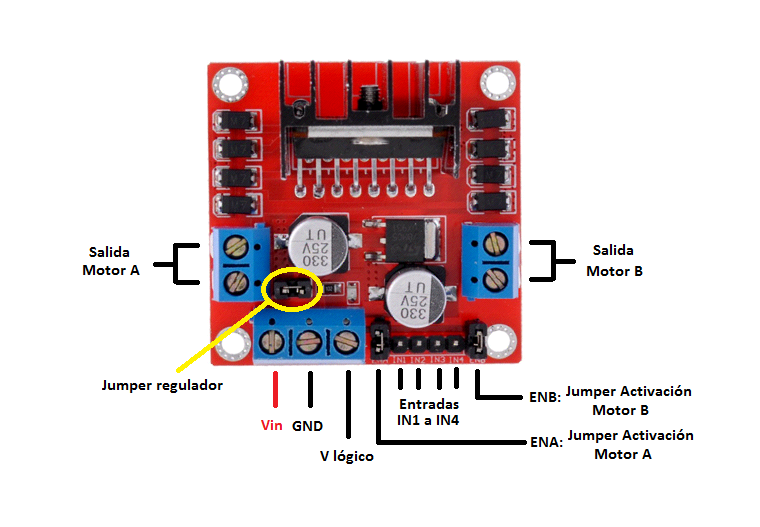
\includegraphics[scale=0.6]{figs/L298N} % Escala la imagen al 150% de su tamaño original
  \caption{Controlador driver L298N.}
  \label{fig:l298n}
\end{figure}

\begin{table}[H]
\begin{center}
\begin{tabular}{|c|c|}
\hline
\textbf{Parámetros} & \textbf{Valores} \\
\hline
Nombre del controlador & L298N \\
Voltaje de alimentación & 6 - 12 V(jumper) \\
Interfaz de comunicación & Pines digitales, CFG y \hyperlink{PWM}{PWM} \\
Corriente máxima de fase(RMS) & 2 x 2 A \\
Pérdida de conducción & 0.9 - 1.5~$\Omega$ \\
Voltaje lógico & 5 V \\
Dimensiones & 5 x 5 x 3 cm \\
Peso & 27 g \\
\hline
\end{tabular}
\caption{Especificaciones técnicas del L298N}
\label{cuadro:ejemplo}
\end{center}
\end{table}

\vspace{2cm}

\subsection{Motores}
\label{subsec:motores}

Un motor reductor es un tipo de motor eléctrico que tiene incorporado un mecanismo de reducción como un engranaje y que sirve para aumentar el torque de salida, es decir, una mayor fuerza en el eje del motor, lo cual es una opción idónea para esta aplicación ya que se necesita mover mucho peso contando con las piezas del robot, la Powerbank, la Raspberry y la batería, disminuyendo la velocidad de rotación y teniendo a su vez un control preciso del motor. La velocidad en este caso no menos importante que la fuerza del motor ya que el objetivo final que pueda desplazarse con todo el peso incorporado para llegar al objetivo final aunque será necesaria controlarla igualmente. \\

En concreto, se han usado dos motores reductores como los que se muestran en la Figura \ref{fig:Motor} junto con dos ruedas de anclaje que encajan perfectamente con los ejes de cada motor, y están a la venta en Amazon por un precio de 11 \euro. 

\begin{figure}[H]
  \centering
  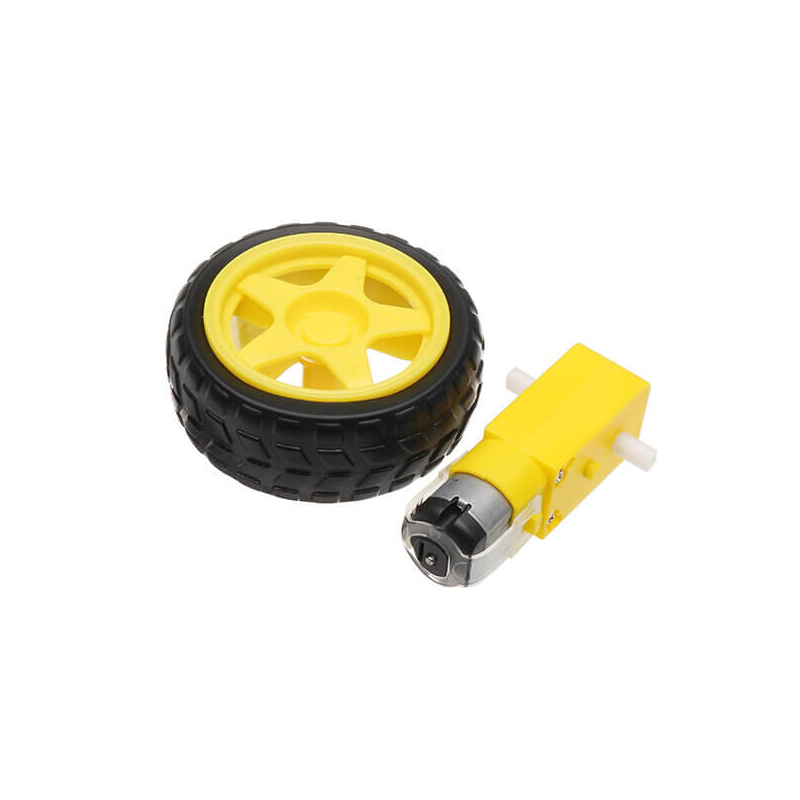
\includegraphics[scale=0.35]{figs/motor} % Escala la imagen al 150% de su tamaño original
  \caption{Motor reductor con rueda de anclaje.}
  \label{fig:Motor}
\end{figure}

\begin{table}[H]
\begin{center}
\begin{tabular}{|c|c|}
\hline
\textbf{Parámetros} & \textbf{Valores} \\
\hline

Nombre del motor & Motor reductor \\
Peso & 20 g \\  
Diámetro del eje & 3 mm \\   
Dimensiones & 70 x 22 x 18mm \\   
Torque de sujeción & 0.0687 Nm Aprox \\
Corriente máxima de fase & 850 mA \\  
Tipo de motor & Corriente continua \\   
Voltaje & 3 - 6 V \\  
Reducción & 48:1 \\ 
Velocidad sin carga & 230 rpm \\ 


\hline
\end{tabular}
\caption{Especificaciones técnicas de los motores}
\label{cuadro:ejemplo}
\end{center}
\end{table}


\subsection{Fuentes de alimentación}
\label{subsec:fuentes_alimentacion}

Para poder alimentar al controlador L298N, se va a necesitar una batería de 6 V y 6 A y que sea recargable como la que se muestra en la 
en la figura \ref{fig:bateria}, ya que se será necesaria su recarga para hacer múltiples pruebas con el robot. Esta batería consta de 5 pilas AA y un cable de carga, con un peso de 129 gramos, lo cual es perfecta para que pueda proporcionar la potencia necesaria para los motores y que a diferencia de las baterías de ácido son más ligeras, ya que éstas, normalmente son más pesadas debido a que están hecas de plomo y ácido.\\

Este tipo de fuentes, se pueden encontrar en páginas como Amazon a un precio de 18 \euro, pero se podían haber usado otras que proporcionasen una alimentación en el rango de 6 - 12 V, siempre y cuando se tenga el jumper del controlador inactivo, porque si estuviese activoo habría que proporcionar una alimentación entre 12 - 35 V como se mencionó anteriormente, pero como los motores necesitan 6 V sólo, pues valdrían con las que se han usado. \\

Por otra parte, habría que alimentar a la Raspberry, ya que el robot se manejará de manera independiente y sin cables de por medio, por lo que se utilizará una Powerbank como la de la figura \ref{fig:Powerbank}, la cual es idónea debido a su peso ligero de 200 gramos y la tensión y amperaje que proporciona de 5 V y 3 A respectivamente, ya que es justo lo que necesita la Raspberry Pi 4 que se va a utilizar para que funcione correctamente y tenga un rendimiento estable.

\begin{figure}[H]
  \begin{minipage}{0.48\textwidth}
    \centering
    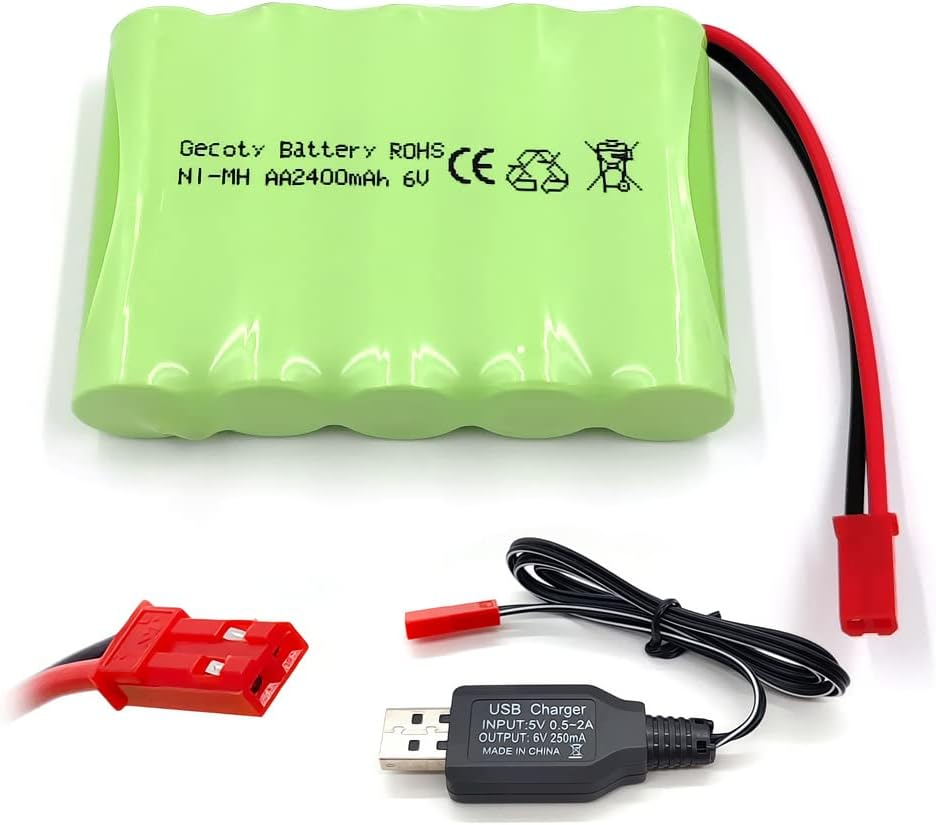
\includegraphics[width=6.5cm]{figs/bateria.jpg}
    \caption{Batería recargable con cable de carga.}
    \label{fig:bateria}
  \end{minipage}
  \hfill
  \begin{minipage}{0.48\textwidth}
    \centering
    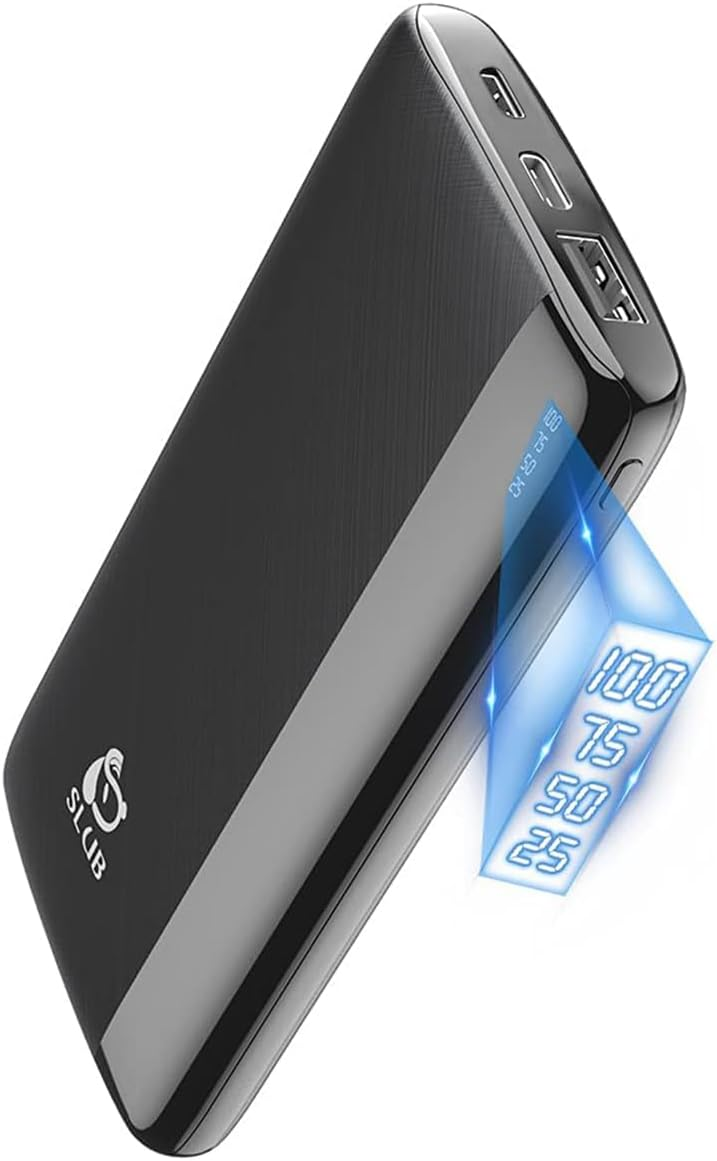
\includegraphics[scale=0.13]{figs/powerbank.jpg}
    \caption{Powerbank.} 
    \label{fig:Powerbank}
  \end{minipage}
\end{figure}

\subsection{Rueda loca}
\label{subsec:rueda_loca}

Para que el robot pueda desplazarse en cualquier dirección sin ningún problema se utilizará una rueda loca como la de la figura \ref{fig:Rueda_loca} imitando el comportamiento de una pelota rodante, la cual irá anclada en la parte trasera del robot con 2 tornillos y 2 tuercas proporcionando al robot un movimiento suave y de baja fricción, de alto rendmiento y larga vida.


\begin{figure}[H]
  \centering
  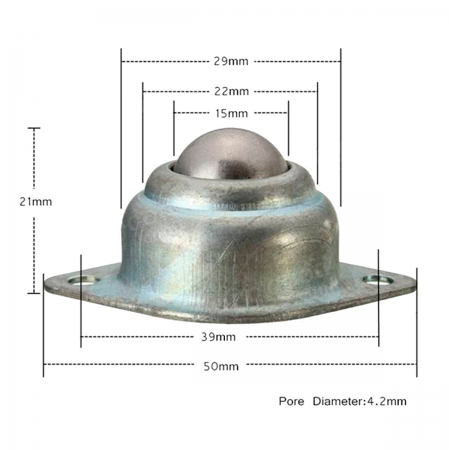
\includegraphics[scale=0.4]{figs/rueda_loca} % Escala la imagen al 150% de su tamaño original
  \caption{Rueda loca para robot.}
  \label{fig:Rueda_loca}
\end{figure}



\subsection{Base principal}
\label{subsec:base_principal}

Primero, habría que pensar en la forma que tiene que tener la base para poder soportar tanto los motores, como la batería, la Raspberry y la Powerbank. Para ello, se diseñará una estructura muy simple en la cual, habrá diferentes cavidades las cuales nos servirán para poder insertar de la manera más fácil posible todo lo que se necesita, como lo mencionado anteriormente más el controlador, sensores, cables y otros huecos para añadir si se requiere en un futuro otro tipo de sensores y actuadores. \\

Finalmente, para el diseño de esta base, habría que hacer uso de FreeCAD \ref{subsec:freecad} para poder imprimir esta pieza y cumplir con el objetivo establecido inicialmente de poder soportar todo el peso posible, y que sea escalable a nivel de que se puedan cualquier cosa para cumplir con objetivos futuros y de esta manera también, al ser completamente Open Source, cualquier persona podrá modificarlo a su manera y utilizarlo de manera gratuita, por lo que quedaría de la siguiente manera como se puede apreciar en esta figura \ref{fig:Base_principal}:

\begin{figure}[H]
  \centering
  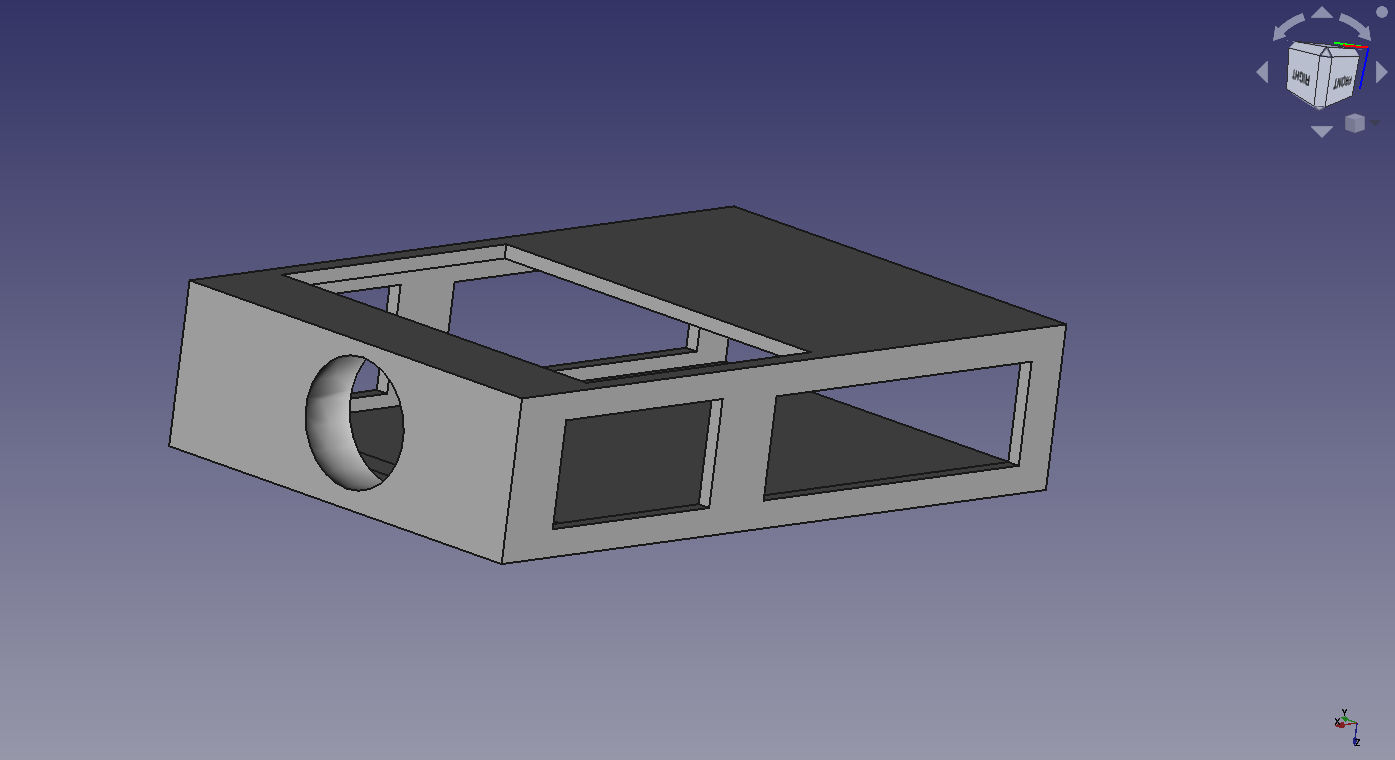
\includegraphics[scale=0.25]{figs/base} % Escala la imagen al 150% de su tamaño original
  \caption{Base principal.}
  \label{fig:Base_principal}
\end{figure}

Como se puede apreciar en la imagen, la cavidad circular sirve por si en algún futuro se desea añadir algún sensor, ya sea como el ultrasonidos. Las dos cavidades rectangulares menores sirven para poder anclar las ruedas a los motores que irán éstos a su vez añadidos a través del hueco rectangular superior. Por otra parte, las dos cavidades rectangulares mayores, junto con el hueco de la parte trasera, sirven para poder introducir la batería y el magnetómetro como se verá más adelante de una manera asequible y sencilla. La Raspberry y la Powerbank irán encima de la parte trasera y el controlador y los cables como no hace faltan que estén sujetos a nada debido a menor peso, irán en el hueco frontal superior encima de los motores.


\subsection{Plataforma hardware}
\label{subsec:plataforma_hardware}


Para poder cumplir con el objetivo establecido de diseñar y controlar un robot guía por voz, con las características que ya se han definido en el capítulo anterior y que a sea también de bajo coste, en este proyecto la infraestrucutra hardware se ha centrado en los sistemas embebidos que hay disponibles en el mercado. En primer lugar, una parte del software, como la de entrenar la red neuronal, se probó con éxito en un sistema operativo Ubuntu 20.04 y el siguiente paso era migrarlo a la Raspberry Pi. En segundo lugar, se intentó probar que funcinonara en una Raspberry Pi 3 Model B+ pero sin éxito, ya que aunque se consiguieron instalar los mismos paquetes con las mismas versiones sin ningún problema, a la hora de instalar en concreto una de las librerías necesarias para transformar y manipular los archivos de audio como la de librosa, se experimentaron problemas de bloqueos y de rendimiento durante días sin ningún cambio apreciable, por lo que seguramente sea por limitaciones de recursos de hardware de este modelo.\\

La Raspberry Pi 3+ tiene especificaciones decentes para muchas tareas, pero ciertas aplicaciones y bibliotecas pueden ser exigentes en términos de procesamiento y memoria, lo que puede conllevar a problemas de rendimiento. La biblioteca librosa es conocida por ser computacionalmente intensiva, especialmente al trabajar con archivos de audio grandes o al realizar operaciones complejas de procesamiento de señales de audio, por lo que se esta opción queda descartada y se llegará a probar en una Raspberry Pi 4 Model B.\\

En general, la Raspberry Pi 4 ofrece un salto significativo en términos de rendimiento y capacidades en comparación con la Raspberry Pi 3 Model B+, ya que tiene un procesador más potente y mucha más RAM (4 GB), lo que la hace más capaz de manejar tareas intensivas y ejecutar aplicaciones más exigentes. Para usarla correctamente, habrá que añadir disipadores de calor y un ventilador, ya que genera más calor que la Raspberry Pi 3.



\begin{figure}[H]
  \centering
  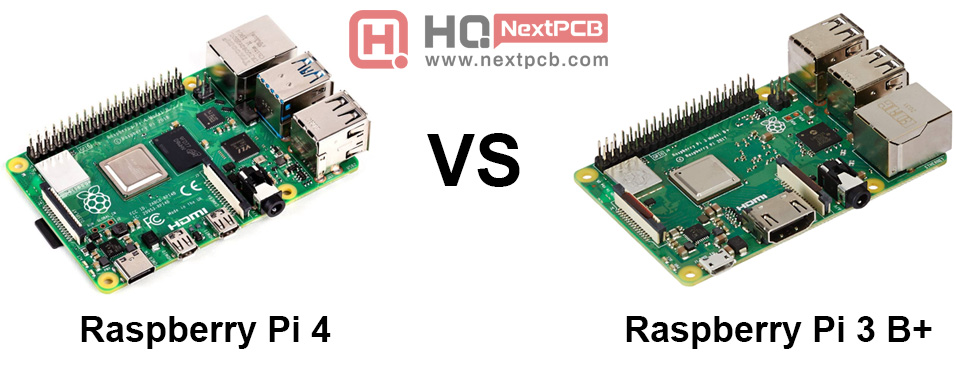
\includegraphics[scale=0.4]{figs/rasps} % Escala la imagen al 150% de su tamaño original
  \caption{Raspberry Pi 4B vs Raspberry Pi 3B+.}
  \label{fig:Raspberry}
\end{figure}


Esta placa tiene pines \hyperlink{GPIO}{GPIO} los cuales permiten que se conecten tanto sensores como actuadores mediante diferentes tipos, como los que se muestran en la figura \ref{fig:Pines}. Hay diferentes tipos de pines:

\begin{itemize}
 \item \textit{GND.} Es usado para poder cerrar el circuito elécctrico y que la corriente pueda fluir adecuadamente entre los dispositivos conectados y no haya ningún daño. Son los pines 6,9,14,20,25,30,34 y 39.
 \item \textit{Pin de 5V.} En los pines 2 y 4 se proporciona una alimentación de 5V.
 \item \textit{Pin de 3V.} En los pines 1 y 17 se proporciona una alimentación de 3V.
 \item \textit{Modulación por ancho de pulso (\hyperlink{PWM}{PWM}).} Se corresponden con los pines 12,32,33 y 35 y permiten modificar el ciclo de tranajo con una señal periódica establecida.
 \item \textit{Conexión \hyperlink{UART}{UART}.} Se corresponden con los pines 8 y 10.
 \item \textit{Conexión \hyperlink{SPI}{SPI}.} Se corresponden con los pines 19,21,23,24 Y 26.
 \item \textit{Conexión \hyperlink{I2C}{I2C}.} Se corresponden con los pines 3(SDA), 5(SCL), 27(SDA) y 28(SCL).	
 \item \textit{} Los demás pines son usados para garantizar la conexión de entrada o salida con el dispositivo conectado. 
\end{itemize}\

\begin{figure}[H]
  \centering
  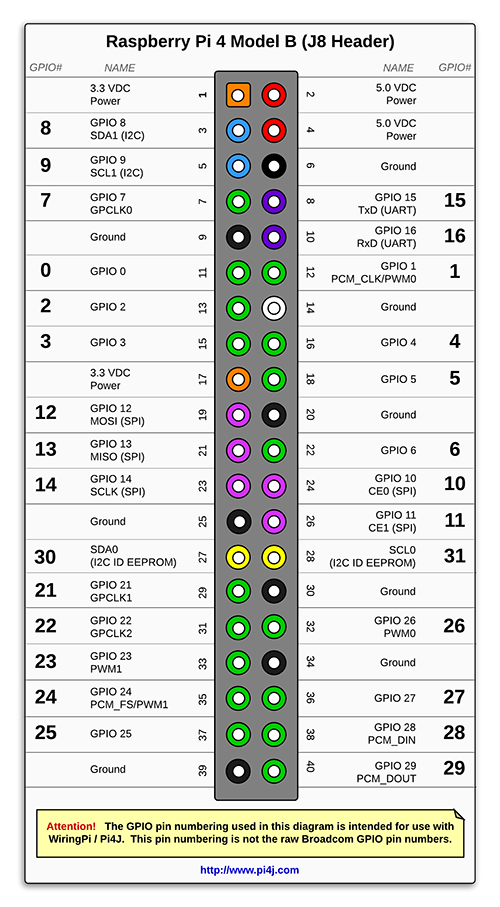
\includegraphics[scale=0.4]{figs/pines} % Escala la imagen al 150% de su tamaño original
  \caption{Diferentes tipos de pines GPIO en Raspberry Pi 4B.}
  \label{fig:Pines}
\end{figure}


\subsection{Magnetómetro}
\label{subsec:magnetómetro}


Para obtener la orientación absoluta del robot se puede usar un sensor como ya se mencionó anteriormente como el mpu9250 que se aprecia en la figura \ref{fig:mpu9250}. Este dispositivo compacto y versátil que combina el acelerómetro de 3 ejes, el giroscopio de 3 ejes y el magnetómetro de 3 ejes en un solo paquete,es decir, por lo puede medir la aceleración lineal, la velocidad angular y la intensidad del campo magnético terrestre en los 3 ejes.\\ \\ Tiene integrado un \hyperlink{DMP}{DMP} capaz de realizar complejos algoritmos de captura de movimiento de los 9 ejes. Este sensor se comunica con microcontroladores a través de la interfaz I2C y posee una librería muy extensa para su uso inmediato e incorpora un regulador de voltaje a 3.3V en la placa y resistencias pull-up para su uso directo por I2C. Para una captura precisa de movimiento rápido y lento, tiene un rango de escala programable de 250/500/1000/2000 grados/seg para el giroscopio, 2g/4g/8g/16g para el acelerómetro y ±4800µT para el magnetómetro.\\ \\
Su magnetómetro incorporado se puede utilizar para estimar el ángulo de orientación absoluta como el de una brújula. Este ángulo conocido como acimut, se refiere a la dirección en la que apunta un objeto o una persona, en relación normalmente con el norte.\\ \\ Una lectura de 0º indicaría una dirección hacia el norte verdadero, 90º, 180º y 270º indicarían este, sur y oeste, respectivamente. Se puede determinar este ángulo utilizando lecturas de un magnetómetro con otras técnicas de calibración para estimar con alta precisión en qué dirección va, resultando así muy útil para que el robot pueda orientarse en interiores.



\begin{figure}[H]
  \centering
  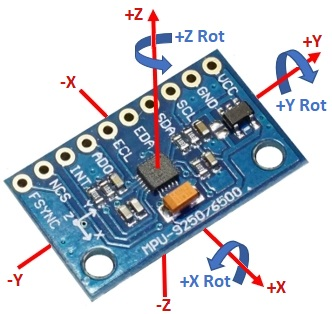
\includegraphics[scale=0.7]{figs/mpu9250} % Escala la imagen al 150% de su tamaño original
  \caption{Sensor MPU9250.}
  \label{fig:mpu9250}
\end{figure}


\begin{table}[H]
\begin{center}
\begin{tabular}{|c|c|}
\hline
\textbf{Parámetros} & \textbf{Valores} \\
\hline

Nombre del sensor & MPU9250 \\
Voltaje de operación & 3.3 - 5 V \\  
Grados de libertad(\hyperlink{DoF}{DoF}) & 9 \\   
Rango de acelerómetro & ±2g, ±4g, ±8g, ±16g \\   
Rango Giroscopio & ±250º/Seg, ±500º/Seg, ±1000º/Seg, ±2000º/Seg \\
Rango Magnetómetro & ±4800 $ \mu $T \\  
Interfaz & I2C y SPI \\   
Conversor AD & 16 Bits (salida digital) \\   
Dimensiones & 25 x 16 x 3mm \\
Consumo de energía(modo activo) & 3.2 mA \\
Temperatura de funcionamiento & -40ºC a +85ºC \\ 


\hline
\end{tabular}
\caption{Especificaciones técnicas del sensor MPU9250}
\label{cuadro:ejemplo}
\end{center}
\end{table}

\section{Software}
\label{sec:software}


Al hacer uso finalmente de una Raspberry Pi 4B, se usó un sistema operativo oficial Raspberry Pi OS conocido como Raspbian(Figura \ref{fig:raspbian}) con la versión de 64 bits y como está basado en Debian, se dispondrá de las cualidades de un sistema Linux. Se ha decidido usar este sistema operativo debido a su optimización para que pueda funcionar en procesadores ARM(el que ya tiene la Raspberry) ofreciendo así el mejor rendimiento posible para este placa.


Posteriormente, se definirán todos las librerías externas y programas que han sido necesarios para poder desarrollar este proyecto correctamente.

\begin{figure}[H]
  \centering
  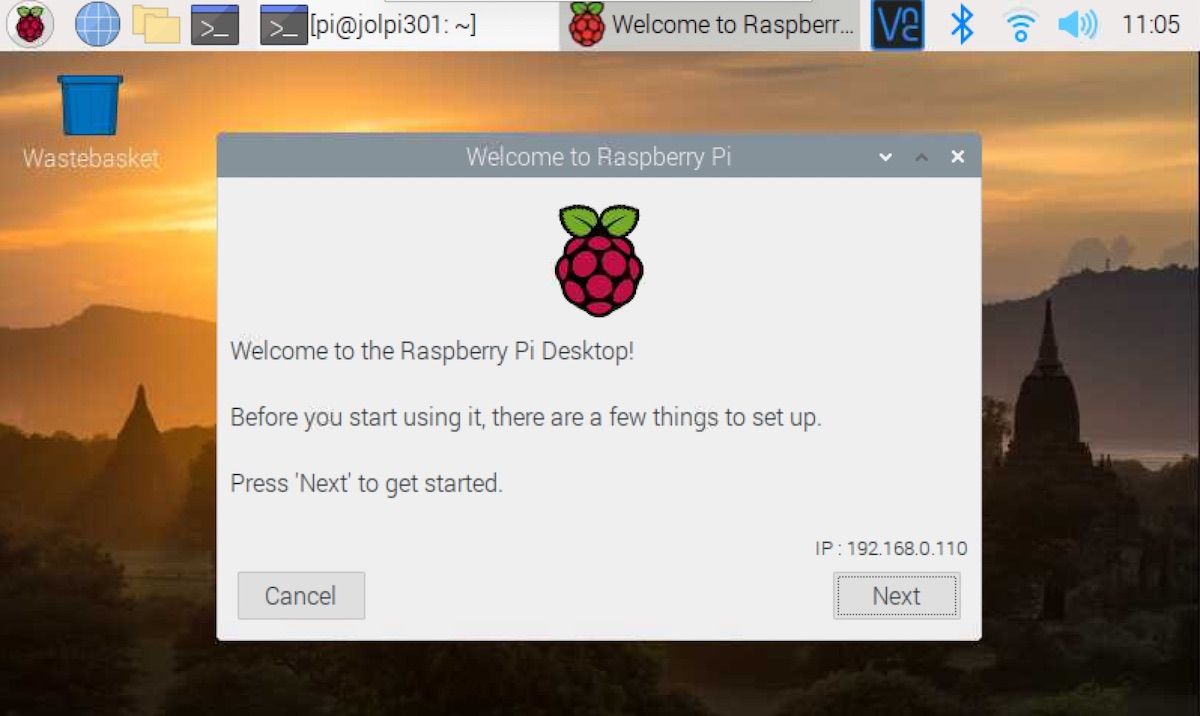
\includegraphics[scale=0.3]{figs/raspbian} % Escala la imagen al 150% de su tamaño original
  \caption{Raspberry Pi OS.}
  \label{fig:raspbian}
\end{figure}


\subsection{Python}
\label{subsec:python}

Python es un lenguaje de programación interpretado de alto nivel y orientado a objetos, es decir, que al ser de alto nivel su nivel de abstracción es más cercano al lenguaje humano que al de una máquina y es de fácil uso en comparación con los lenguajes de bajo nivel. Es interpretado en el sentido que es un intérprete el que ejecuta línea por línea en vez de ser compilado a código máquina previamente como en C o C++. Es uno de los lenguajes de programación más usados en el mundo debido a su amplia librería estándar, garantizando así multitud de funciones y módulos para realizar difentes tareas y a suz vez, está soportado de manera nativa por el sistema operativo utilizado Raspbian.\\ \\ También cuenta con una gran variedad de librerías de terceros como Numpy para cálculos numéricos, Pandas para el análisis de datos, librosa para la manipulación de datos de auido lo cual será de gran ayuda a la hora de entrenar la red neuronal con los comandos, seaborn para la visualización de datos estadísticos, entre otros. En este proyecto, Python se usará para leer y procesar los datos de los sensores de manera concurrente proporcionando órdenes a los actuadores para alcanzar un objetivo en concreto.



\subsection{FreeCAD}
\label{subsec:freecad}


FreeCAD es una herramienta de software libre y gratuito el cual es usado para modelar y diseñar piezas en 3D para posteriormente ser impresas. Su modelo se basa en usar una serie de parámetros para poder construir modelos en 3D para que se puedan modificar de una manera sencilla. Entre las ventajas que tiene este programa de diseño, está la de tener un banco de trabajo, el cual es un conjunto de herramientas especializadas para poder realizar una tarea específica dentro del software como el modelado paramétrico. 


\begin{figure}[H]
  \centering
  
\includegraphics[scale=0.3]{figs/freecad} % Escala la imagen al 150% de su tamaño original
  \caption{Logo de FreeCAD.}
  \label{fig:freecad}
\end{figure}


La comunidad también es capaz por otra parte de agregar nuevas herramientas y funciones al software, por lo que esta herramienta va mejorando continuamente y no es muy difícil de entender y aprender todos los conceptos necesarios para poder usarla correctamente debido a toda la documentación que hay junto con los tutoriales correspondientes.


\subsection{Scikit-learn}
\label{subsec:sklearn}


Scikit-learn es probablemente la biblioteca más útil para el aprendizaje automático de software libre en Python. La biblioteca sklearn contiene muchas herramientas eficientes para el aprendizaje automático y el modelado estadístico, incluidas la clasificación, la regresión, la agrupación y la reducción de la dimensionalidad.\\ Para este proyecto, se usarán partes específicas de este biblioteca para así evitar cargar todo el módulo entero y para hacer el código más claro ya que se importa sólo lo que se necesita. \\

En concreto, se usarán las partes para escalar o normalizar las características antes de entrenar el modelo, para implementar diferentes algoritmos de aprendizaje automático y funciones para dividir el conjunto de datos en diferentes subconjuntos de datos de entrenamiento, que son los que se han utilizado para entrenar el modelo y de pueba, que son los que se han utilizado para poder evaluar el modelo y verificar su capacidad de una manera más eficiente.\\

También proporcionará varias métricas que se pueden utilizar para poder evaluar el rendimiento de los diferentes modelos o algoritmos de clasificación, resultando así muy útil para elegir de modelo final para el entrenamiento de la red neuronal.

\begin{figure}[H]
  \centering
  
\includegraphics[scale=0.1]{figs/sklearn} % Escala la imagen al 150% de su tamaño original
  \caption{Logo de la biblioteca Scikit-learn.}
  \label{fig:sklearn}
\end{figure}

\subsection{Librosa}
\label{subsec:librosa}

Librosa es un paquete de Python para el análisis y procesamiento de música y audios. De esta manera, proporciona las herramientas necesarias para poder extraer las características y la manipulación de un audio y la respectiva visualización de los datos del sonido del mismo. En concreto servirá para calcular el espectograma de un audio que es una representación visual en la que se muetran la intensidad de señal del audio y la frecuencia a través de la \hyperlink{STFT}{STFT}, permitiendo analizar así cómo va cambiando la frecuencia con el tiempo.\\

También permite calcular el cronograma de un audio que es una representación de la intensidad de todas las notas musicales que están presentes en un audio y a su vez, calcular los coeficientes de \hyperlink{MFCC}{MFCC} de un audio que son las características más importantes de un audio respecto con la percepción sonora del humano sobre ese audio.\\ \\

En resumen, con todas estas características de cada audio por voz, se podrán usar los modelos de clasificación para predecir la clase a la que pertenece cada audio. 

\begin{figure}[H]
  \centering
  
\includegraphics[scale=0.4]{figs/librosa} % Escala la imagen al 150% de su tamaño original
  \caption{Logo del paquete Librosa.}
  \label{fig:librosa}
\end{figure}


\subsection{Smbus2 y mpu9250\_jmdev}
\label{subsec:smbus2mpu9250jmdev}


Smbus2 es una biblioteca la cual es una versión mejorada de la biblioteca smbus y es utilizada en general para la comunicación con los dispositivos I2C como en este caso que es el MPU9250 para calcular la orientación del robot. Tiene un enfoque distinto al de la biblioteca mpu9250\_jmdev en cuanto a la implementación para poder interactuar con el MPU9250 a través de I2C, ya que la primera se usa para poder acceder a los registros del sensor de una manera más manual y escribir todas las funciones necesarias para la lectura de los valores del mismo teniendo así un control sobre el hardware pero se requiere tener un conocimiento pleno de este protocolo y de cómo funciona este sensor.\\

En cambio, la biblioteca mpu9250\_jmdev abstrae la comunicación con los registros de esta comunicación, proporcionando así una clase la cual ya tiene implementada todos los métodos de alto nivel necesarios para poder interactuar con el dispositivo y obtener los datos del giroscopio, acelerómetro, y magnetómetro ,simplificando así el proceso de escribir y leer en los registros del MPU9250 como se hacía con la anterior biblioteca y de esta manera no se profundiza demasiado en el protocolo y teniendo así un enfoque mucho más directo y simple.

\subsection{Jupyter Notebook}
\label{subsec:Jupyter}

Jupyter Notebook es un entorno web interactivo que permite a los usuarios crear y compartir documentos que contienen código en tiempo real, visualizaciones y texto narrativo. De esta manera, todo el entorno que tiene el usuario se podrá visualizar en esta herramienta mediante una interfaz amigable y permitiendo a su vez ejecutar celdas de código de manera individual como se puede apreciar en esta imagen \ref{fig:jup2}, lo que facilita a su vez el análisis paso a paso y ver los resultados de cada celda al momento.\\

\begin{figure}[H]
  \centering
  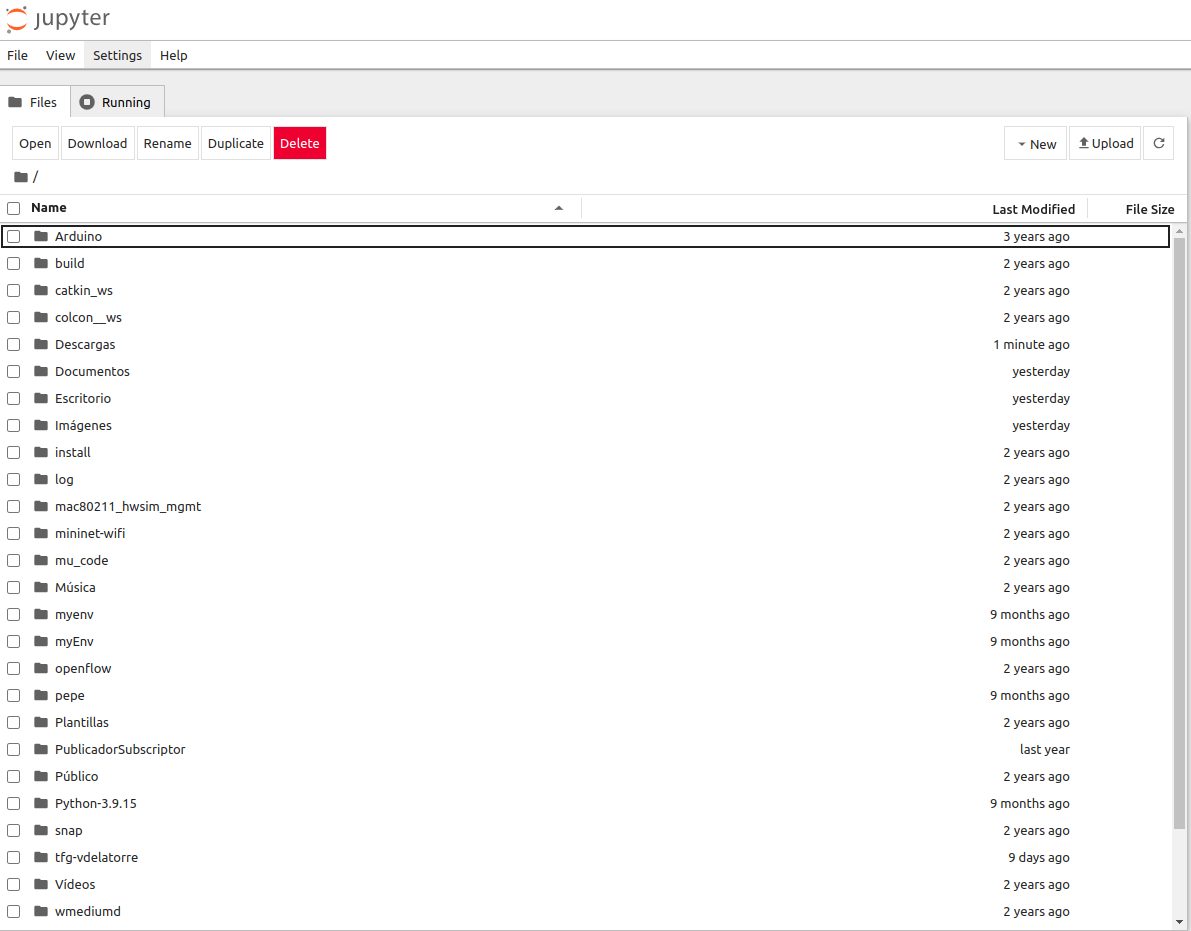
\includegraphics[scale=0.4]{figs/jup1} % Escala la imagen al 150% de su tamaño original
  \caption{Interfaz Jupyter Notebook.}
  \label{fig:jup1}
\end{figure}

Esta herramienta también sirve para manejar bases de datos de prueba y entrenamiento con modelos de aprendizaje automático, ya que se pueden cargar datos y procesarlos de manera interactiva, lo cual será muy útil para hacer las correspondientes pruebas sobre cuántos APs son necesarios para que el robot pueda localizarse como se verá más adelante, ya que para esto se necesitará recoger una gran cantidad de datos de cada APs para que cada modelo procese todo y entorno será de gran ayuda.




\begin{figure}[H]
  \centering
  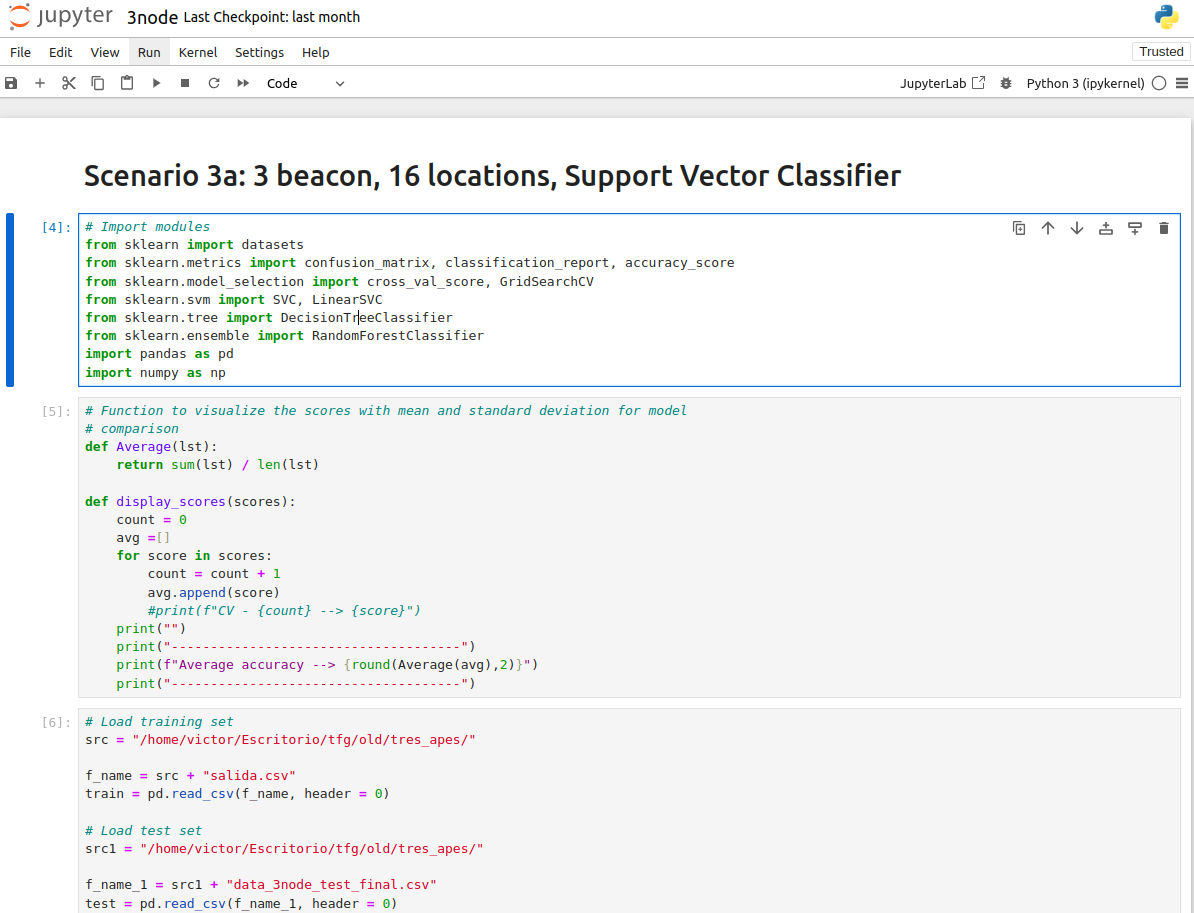
\includegraphics[scale=0.4]{figs/jup2} % Escala la imagen al 150% de su tamaño original
  \caption{Ejemplo de un programa en Jupyter Notebook.}
  \label{fig:jup2}
\end{figure}

\subsection{GIMP}
\label{subsec:gimp}

GIMP es un programa de edición de imágenes de software libre y gratuito en el cual se pueden editar imágenes digitales en forma de mapa de bits, tanto fotografías como dibujos. Para este proyecto, se usará para diseñar el mapa del robot, es decir, dibujar en una imagen píxel a píxel los obstáculos por donde no podrá desplazarse el robot. Para ello se puede hacer uso de las diferentes herramientas como el pincel, lápiz o el borrador y después una vez dibujado el mapa se podrá exportar como una imagen en un formato determinado y ejecutar un programa que hace uso de la Clase Image del módulo PIL que es una biblioteca para trabajar con imágenes en Python y de esta manera poder abrir la imagen, obtener sus dimensiones e iterar sobre cada píxel para escribir la representación binaria, guardarla en formato txt y así esta matriz será la que se le pasará al algoritmo A* para encontrar el camino más óptimo.


\paragraph{Bibliotecas auxiliares utilizadas} \hspace{0pt} \\

A parte de los módulos y bibliotecas mencionadas anteriormente, también se usaron otras herramientas de propósito general. La biblioteca \texttt{threading} la cual se usó para implementar programación concurrente y poder manejar diferentes programas a la vez, como la obtención del ángulo de orientación, mientras que \texttt{subprocess} sirvió para ejecutar comandos externos desde Python, como ejecutar el comando para conectarse a una red WiFi o para grabar un archivo de audio. Para el análisis y manipulación de los datos de audio, se usaron \texttt{pandas} y \texttt{numpy}, que son ampliamente usadas en el ámbito científico. La biblioteca \texttt{heapq} facilitó la gestión eficiente de las estructuras de datos basadas en montículos(heaps), que en este caso se usó sobre todo para manejar el algoritmo A* de una manera más óptima y \texttt{deque} se usó para obtener las útimas lecturas del magnetómetro. Finalmente, se utilizó \texttt{matplotlib.pyplot} para generar y guardar imágenes que ilustraban los resultados obtenidos del algoritmo.\\

Se recomienda instalar todos los paquetes necesarios en un entorno virtual que es un directorio con su propia instalación de Python y sus paquetes, ofreciendo así un control preciso sobre las dependencias de software, el aislamiento de entornos de trabajo y la capacidad de experimentar y probar configuraciones sin afectar al sistema operativo principal, por lo que sería útil instalar la biblioteca \texttt{virtualenv}.




\chapter{Arquitectura software}
\label{cap:capitulo5}

\begin{flushright}
\begin{minipage}[]{10cm}
\emph{Somos lo que hacemos repetidamente, por lo que la excelencia no es un acto, sino un hábito}\\
\end{minipage}\\

Charles Duhigg, \textit{El poder de los hábitos}\\
\end{flushright}

\vspace{1cm}


En este capítulo se describe la topología del sistema utilizado, tanto a nivel software como a nivel hardware. También se describe la forma en la que los diferentes elementos software se complementan, explicando cómo funcionan juntos y detallando los aspectos más importantes de cada uno de ellos.


\section{Estructura hardware}
\label{sec:estructura_hardware}


Para este proyecto se ha usado la Raspberry Pi 4B, debido a su bajo coste y su capacidad de potencia y rapidez con respecto al modelo anterior. El sistema operativo utilizado ha sido Raspbian con la versión de 64 bits. Para la conexión de los diferentes sensores y actuadores se han utilizado los puertos GPIO ya presentados en la sección \ref{subsec:plataforma_hardware}. En la Figura \ref{fig:circuito} se pueden apreciar las diferentes conexiones de los sensores y actuadores a la Raspberry. A continuación se explicarán los detalles de las conexiones de estos componentes hardware :


\begin{itemize}
 \item \textit{Magnetómetro (Figura \ref{fig:mpu9250}).} Este sensor necesita dos pines SDA y SCL, ya que funciona por conexión I2C, por lo que siguiendo el esquema de la Figura \ref{fig:circuito}, se ha conectado a los pines 3 y 5 respectivamente. También se ha conectado al pin 39(GND) para la toma de tierra y al pin 4 para tener la alimentación de  5V. 
 \item \textit{Micrófono micro USB (Figura \ref{fig:microfono-usb}).} Este sensor se ha conectado en el puerto USB que ofrece la Raspberry de entre los 4 que hay.
 \item \textit{Controlador driver L298N (Figura \ref{fig:l298n}).} Este módulo hardware tiene conectados a la Raspberry los terminales ENA, ENB, IN1, IN2, IN3, IN4 y ENB a los pines 32, 36, 35, 38, 37 y 12 respectivamente. También tiene conectados los terminales GND y VCC a los dos pines de la batería recargable y el mismo terminal GND al pin 34 (GND). Ambos pines de cada motor deben ir conectados a los pines de salida del controlador, OUT1 Y OUT2 para un motor y OUT3 y OUT4 para el otro.
 \item \textit{Powerbank (Figura \ref{fig:Powerbank}).} Esta fuente de alimentación irá conectada al puerto USB-C para proporcionar a la Raspberry los 5V y 3A necesarios.
\end{itemize}\


\begin{figure}[H]
  \centering
  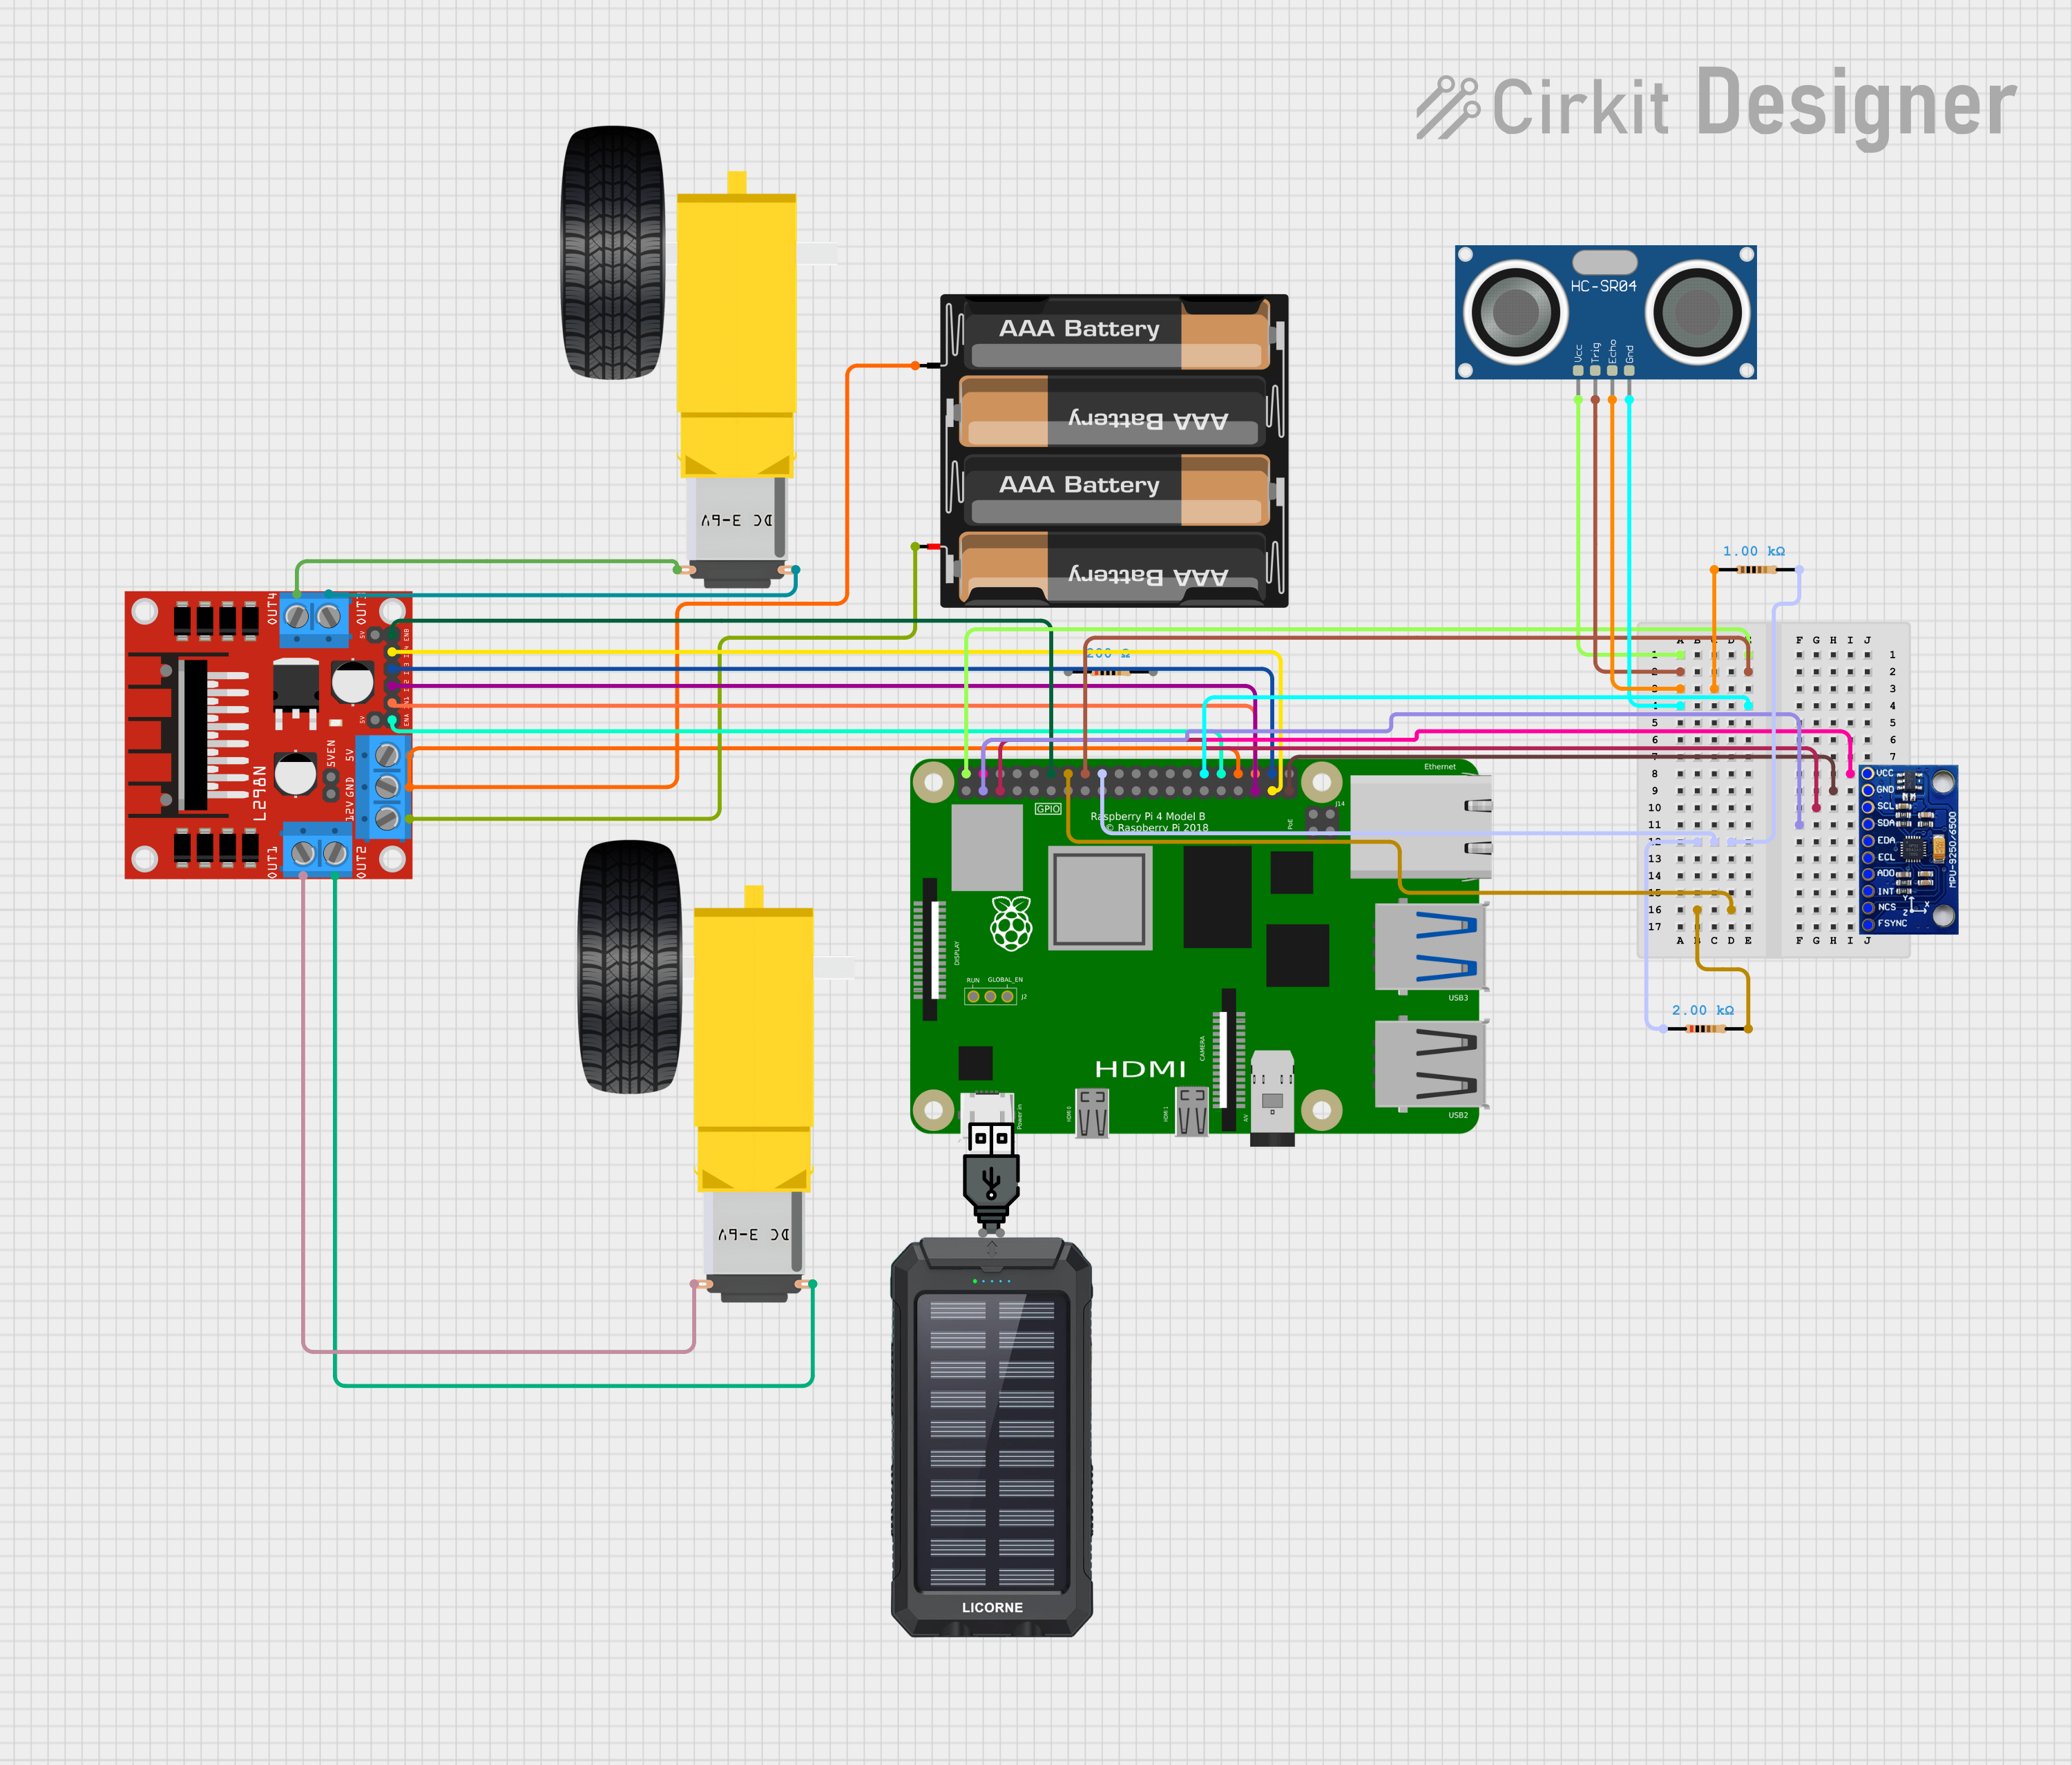
\includegraphics[scale=0.5]{figs/final_circuito} % Escala la imagen al 150% de su tamaño original
  \caption{Esquema de conexiones.}
  \label{fig:circuito}
\end{figure}

\section{Desarrollo software}
\label{sec:desarrollo_software}

Después de diseñar la plataforma hardware, el siguiente paso será darle soporte software, por lo que será necesario calcular el ángulo de orientación del robot, la localización en el mapa, proporcionar un algoritmo que calcule la ruta óptima, y que funcione la red neuronal con distintos comandos por voz, entre otras cosas.


\subsection{Orientación del robot}
\label{subsec:orientacion_robot}

Para poder realizar giros más precisos y tener una trayectoria controlada del robot, es necesario calcular el ángulo de orientación de este dispositivo MPU9250, que como ya se mencionó anteriormente, cuenta con un magnetómetro de 3 ejes, por lo que, utilizando estas lecturas con otras técnicas de calibración, se podrá estimar con alta precisión en que dirección va. Para ello, habrá que actualizar la lista de paquetes, instalar el administrador de paquetes de Python \verb|python3-pip|  e instalar la biblioteca \verb|smbus2| necesaria para I2C, y también la biblioteca \verb|mpu9250-jmdev| específicamente para el MPU9250.



Por otra parte, es muy importante activar el protocolo de I2C para que se pueda comunicar con la Raspberry y le pueda transmitir los datos adquiridos. Esto se activa en: Preferences \texttt{->} Raspberry Pi Configuration \texttt{->} Interfaces \texttt{->} I2C. Si estaba desactivada, es necesario reiniciar la Raspberry. Una vez hecho esto, para ver si lo ha reconocido bien el sensor, habría que ejecutar el comando i2cdetect -y 1 el cual dará una tabla que muestra las direcciones I2C de los dispositivos detectados, y habrá que comprobar que detectó un dispositivo. Como se puede apreciar en la Figura \ref{fig:bus}, lo detectó en la dirección 0x68.


\begin{figure}[H]
  \centering
  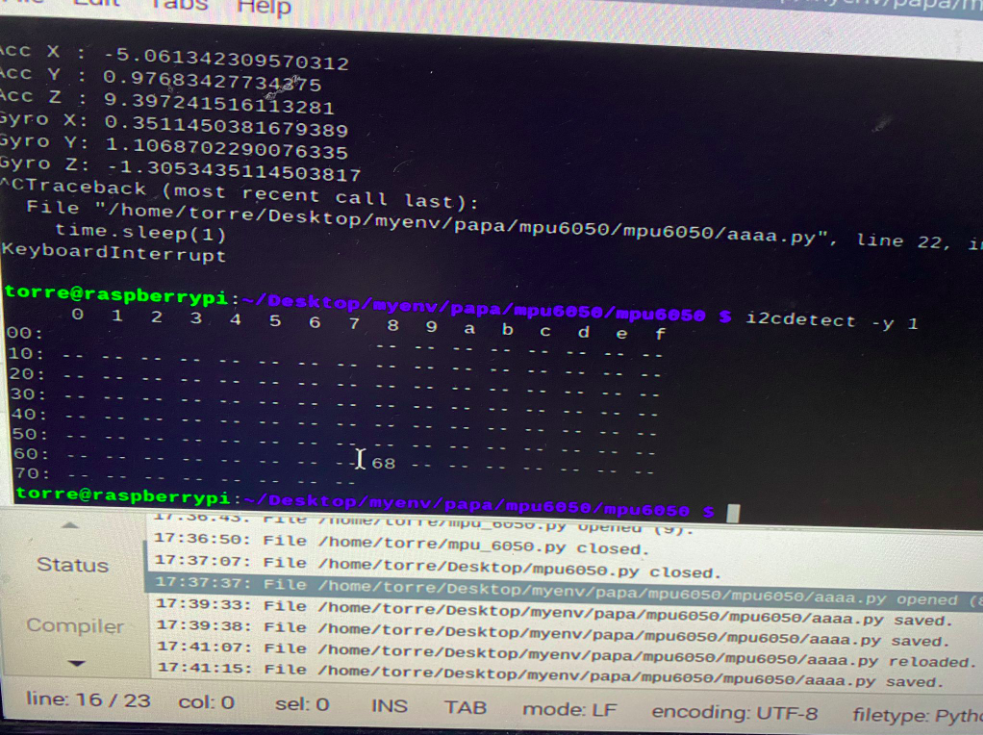
\includegraphics[scale=0.3]{figs/bus} % Escala la imagen al 150% de su tamaño original
  \caption{ Direcciones I2C de los dispositivos detectados.}
  \label{fig:bus}
\end{figure}

El siguiente paso sería obtener las lecturas del magnetómetro. Para ello, habrá que hacer uso de la clase \ref{cod:codejemplo} proporcionada por la biblioteca \texttt{mpu9250\_jmdev}. En primer lugar, se crea una instancia de esta clase con el constructor, con una serie de parámetros que definen la configuración del sensor, que son los siguientes:

\begin{itemize}
 \item \textit{Address\_ak:} Esta es la dirección la cual especifica dónde está conectado el magnetómetro en el bus I2C cuyo valor por defecto es \texttt{AK8963\_ADDRESS}.
 \item \textit{Address\_mpu\_master:} Esta es la dirección I2C del MPU9250 cuyo valor por defecto es \texttt{MPU9050\_ADDRESS\_68}.
 \item \textit{Address\_mpu\_slave:} Esta es la dirección I2C del MPU9250 esclavo si existe, es decir, si se usa un segundo dispositivo cuyo valor por defecto es \texttt{None}.
 \item \textit{Bus:} Este es el número del bus I2C que por defecto es 1.
 \item \textit{Gfs:} Este es el rango de sensibilidad del giroscopio que por defecto es \texttt{GFS\_2000 ($\pm 2000^\circ$/seg)}.
 \item \textit{Afs:} Este es el rango de sensibilidad del acelerómetro que por defecto es \texttt{AFS\_16G ($\pm 16G$)}.
 \item \textit{Mfs:} Este es el rango de sensibilidad del magnetómetro que por defecto es \texttt{AK8963\_BIT\_16 (16 bits)}.
 \item \textit{Mode:} Este es el modo de operación del magnetómetro el cual establece el modo de funcionamiento y la frecuencia de muestreo cuyo valor por defecto es \texttt{AK8963\_MODE\_C100HZ}.
\end{itemize}


Luego se configura el sensor para inicializarlo con los parámetros dados mediante el método \verb|configure(self, retry=3)|. El parámetro retry es el número de intentos para configurar el sensor que por defecto vale 3 por si ocurre algún error en la configuración, pues se intenta de nuevo las veces que el parámetro retry diga. Dentro de este método, se llama a \verb|configureMPU6500(gfs, afs)| para configurar el giroscopio y acelerómetro con las escalas determinadas y también se llama a \verb|configureAK8963(mfs, afs)| para configurar el magnetómetro con el modo y la resolución especificadas y si se agotan los intentos dando error en todos se lanza una excepción.\\


A continuación se leen los datos del magnetómetro con la función \verb|readMagnetometerMaster(self)| para obtener los 3 componentes del campo magnético medidos en cada uno de los ejes. Primero verifica si hay algún MPU9250 esclavo conectado con el método \verb|hasSlave()| y si lo hay, lee los datos desde el esclavo con la función \verb|readMaster(EXT_SENS_DATA_14, 7)|, el primer parámetro se corresponde con una dirección específica de un registro en el MPU9250 y el segundo es la cantidad de bytes que se quieren leer.\\

Si no hay ningún esclavo conectado, lee los datos directamente del magnetómetro con la función \verb|readAK(AK8963_MAGNET_OUT, 7))| siendo similar a la anterior. Finalmente, los datos leídos se convierten a unidades compatibles con el método \verb|convertMagnetometer(data)| y si ocurre algún error al leerlos devuelve un valor de error definido por la función \verb|getDataError()|.\\

Para esta aplicación, solamente se hará uso de las componentes x e y, ya que el objetivo es determinar la dirección del norte magnético en el plano horizontal. La componente z no se utiliza ya que no aporta información relevante, ya que funciona igual que una brújula y ésta misma mide la dirección en el plano horizontal con el ángulo calculado en el plano XY.


\begin{code}[H]
\begin{lstlisting}[language=Python]
class MPU9250:
    def __init__(self, 
        address_ak=AK8963_ADDRESS, 
        address_mpu_master=MPU9050_ADDRESS_68, 
        address_mpu_slave=None, 
        bus=1, 
        gfs=GFS_2000, 
        afs=AFS_16G, 
        mfs=AK8963_BIT_16, 
        mode=AK8963_MODE_C100HZ
    )
       
    def configure(self, retry=3):
        try:
            self.configureMPU6500(self.gfs, self.afs)
            self.configureAK8963(self.mfs, self.mode)
        except OSError as err:
            if(retry > 1):
                self.configure(retry - 1)
            else:
                raise err
     
    def readMagnetometerMaster(self):
        try:
            data = None
            if self.hasSlave():
                data = self.readMaster(EXT_SENS_DATA_14, 7)          
            else:   
                data = self.readAK(AK8963_MAGNET_OUT, 7)
            return self.convertMagnetometer(data)
        except OSError:
            return self.getDataError()           
\end{lstlisting}
\caption[Clase MPU9250]{Clase MPU9250}
\label{cod:codejemplo}
\end{code}


Finalmente, para calcular el ángulo de orientación, habrá que hacer uso de la función \verb|math.atan2(y,x)| para calcular el ángulo entre el vector formado por los parámetros XY y el eje positivo X, siendo x e y las lecturas magnéticas medidas por el magnetómetro. Este ángulo está en radianes por lo que habría que pasarlo a grados multiplicando por 180 y dividiendo entre \(\pi\).\\

La función \verb|math.atan2(y,x)| puede devolver un valor negativo en ciertos casos, y lo ideal es que se mantenga en el rango de 0º y 360º mediante esta condición \ref{cod:codejemplo3}.


\begin{code}[H]
\begin{lstlisting}[language=Python]
if heading_angle_in_degrees < 0:
    heading_angle_in_degrees += 360
\end{lstlisting}
\caption[Mantener el ángulo en el rango correcto]{Mantener el ángulo en el rango correcto}
\label{cod:codejemplo3}
\end{code}


Es importante tener en cuenta también el concepto de declinación magnética, que es el ángulo que existe entre el norte verdadero(Polo Norte geográfico) y el norte magnético que es la dirección hacia el Polo Norte magnético que cambia con el tiempo. Una brújula normal apunta al norte magnético y no al norte verdadero. En este proyecto no se tendrá en cuenta esta desviación, que es diferente dependiendo del lugar, ya que al ser en interiores no varía casi nada este factor pero si fuese en exteriores sí que habría que tenerlo en cuenta. Para saber la declinación magnética de un lugar específico de la Tierra se puede hacer uso de esta página web\footnote{\url{https://www.magnetic-declination.com/}}.\\


Una vez obtenido el ángulo de orientación, se comprueba que las medidas no son exactas y varían mucho, por lo que es necesario calibrar el dispositivo como se muestra en la Sección \ref{sec:cal_mag}.



\subsection{Diseño del mapa}
\label{subsec:diseño_mapa}

Dentro de la navegación global, el robot parte de un mapa conocido gestionado de la siguiente forma. Primero, se hace uso de la herramienta GIMP, como ya se mencionó en la Sección \ref{subsec:gimp} para la edición de imágenes, en la que se tendrá un fondo en blanco y se pintarán de color negro aquellos píxeles que representen obstáculos para el robot y también los APs como se puede apreciar en la Figura \ref{fig:mapa_apes}, ya que se consideran obstáculos por donde no podrá pasar el robot\footnote{En este caso se pintaron de azul para poder distinguirse de un obstáculo normal aunque en el mapa final irán pintados en color negro}.

\begin{figure}[H]
  \centering
  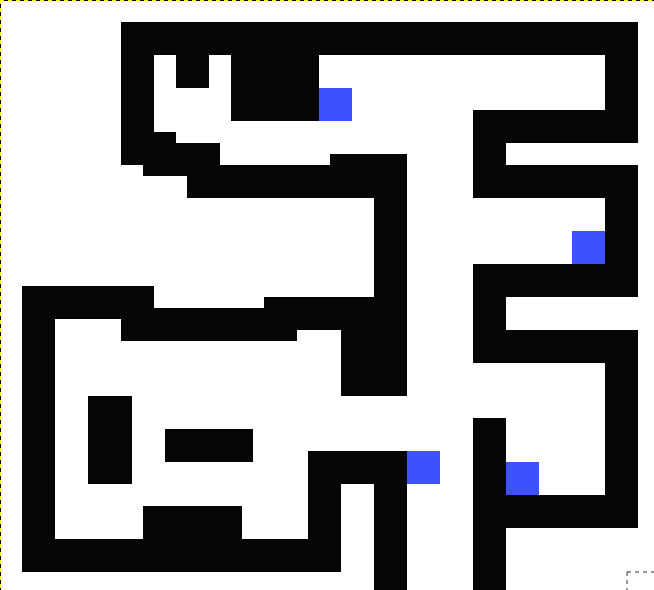
\includegraphics[scale=0.3]{figs/mapa_apes} % Escala la imagen al 150% de su tamaño original
  \caption{ Mapa de ejemplo en GIMP con los APs establecidos.}
  \label{fig:mapa_apes}
\end{figure}

Los píxeles de alrededor de estos obstáculos también se pintarán de color negro para tener un margen de seguridad en los cálculos de movimiento junto con los APs como se puede apreciar en este mapa de ejemplo final (Figura \ref{fig:mapa_apes}):


\begin{figure}[H]
  \centering
  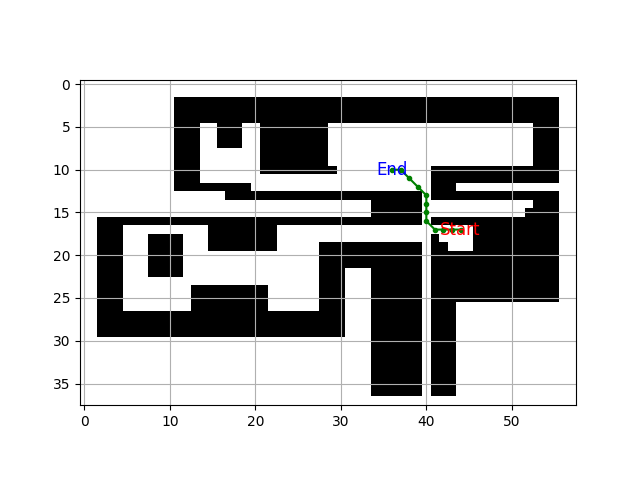
\includegraphics[scale=0.8]{figs/astar} % Escala la imagen al 150% de su tamaño original
  \caption{ Ejemplo del mapa final con los obstáculos ampliados.}
  \label{fig:astar}
\end{figure}

Los colores de cada píxel del mapa tienen importancia y se ha diseñado así ya que el algoritmo de navegación trabaja con una matriz de 0 y 1 por la cual navegará el robot por los valores de la matriz que tienen un 1 que representa el color blanco. Una vez exportada la imagen en formato png, se hará uso de esta función \ref{cod:codejemplo4}, la cual recorre los píxeles de la imagen viendo los valores de cada uno y escribe un 0 o 1 dependiendo del color del píxel, aceptando como parámetros la imagen y un archivo vacío en formato txt en la que se escribirá la matriz.

\begin{code}[H]
\begin{lstlisting}[language=Python]
def image_to_binary_text(image_path, output_file):
    # Abrir la imagen en blanco y negro
    img = Image.open(image_path).convert('1') 

    width, height = img.size
   
    with open(output_file, 'w') as f:
        # Iterar sobre cada pixel de la imagen
        for y in range(height):
            for x in range(width):
                pixel = img.getpixel((x, y))

                bit_value = '0' if pixel == 0 else '1'

                f.write(bit_value)

            f.write('\n') 
\end{lstlisting}
\caption[Función para convertir una imagen en representación binaria ]{Función para convertir una imagen en representación binaria}
\label{cod:codejemplo4}
\end{code}

Finalmente el archivo de salida con la representación binaria de la matriz (Figura \ref{fig:bin}) es la que se le pasará al algoritmo de navegación A* para poder navegar por ella. 

\begin{figure}[H]
  \centering
  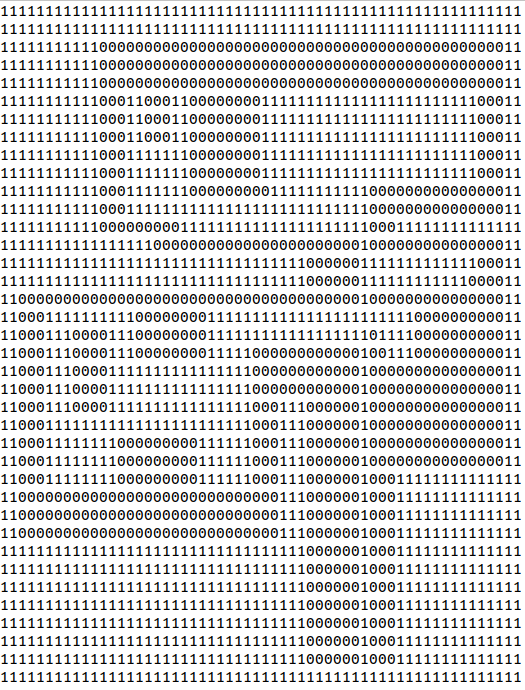
\includegraphics[scale=0.5]{figs/bin} % Escala la imagen al 150% de su tamaño original
  \caption{ Ejemplo de la representación binaria del mapa.}
  \label{fig:bin}
\end{figure}


\subsection{Interfaz de usuario}
\label{subsec:interfaz_usuario}

Una de las mejores formas de interactuar con el robot es mediante comandos de voz ya que es muy natural e intuitivo para los usuarios. El primer paso sería tener un dataset de audios de prueba en español con los comandos de voz que reconocerá el robot. Estos audios deben ir en formato WAV, ya que a diferencia del formato MP3, el formato WAV es un formato de audio sin pérdida, por lo que no hay compresión con pérdida de información auditiva y cada vez que un archivo MP3 se comprime, se pierde cierta información para reducir el tamaño del archivo y podría afectar la calidad del sonido y al rendimiento de la red neuronal si la calidad del audio es crucial y en este caso sí lo es. Al no haber pérdidas en el formato WAV, aumentan los bytes de cada audio por lo que para que se puedan clasificar correctamente, tras diferentes pruebas realizadas cada audio no podrá superar los 200 bytes.\\

Las clases deberían estar equilibradas para facilitar la tarea de entrenamiento; es decir, debería de haber el mismo número de audios para cada clase. Cada audio tiene asignado un número que representa la clase a la que pertenece, como por ejemplo \texttt{ej1-01-.wav}. Las diferentes clases representan los diferentes comandos que hay.\\


 El siguiente paso sería cargar cada uno de los audios y extraer las características de cada uno de ellos para calcular la transformada de Fourier del espectrograma del audio (STFT), los coeficientes cepstrales de frecuencias mel (MFCC) y los espectrogramas mel, ya que son propiedades que usará el modelo para clasificar cada archivo de audio. Para calcular estas características, primero se calcula la forma de onda para diferentes audios (Figura \ref{fig:onda}), y se puede observar que hay una diferencia visible, pero no la suficiente para clasificarla.
 
 \begin{figure}[H]
  \centering
  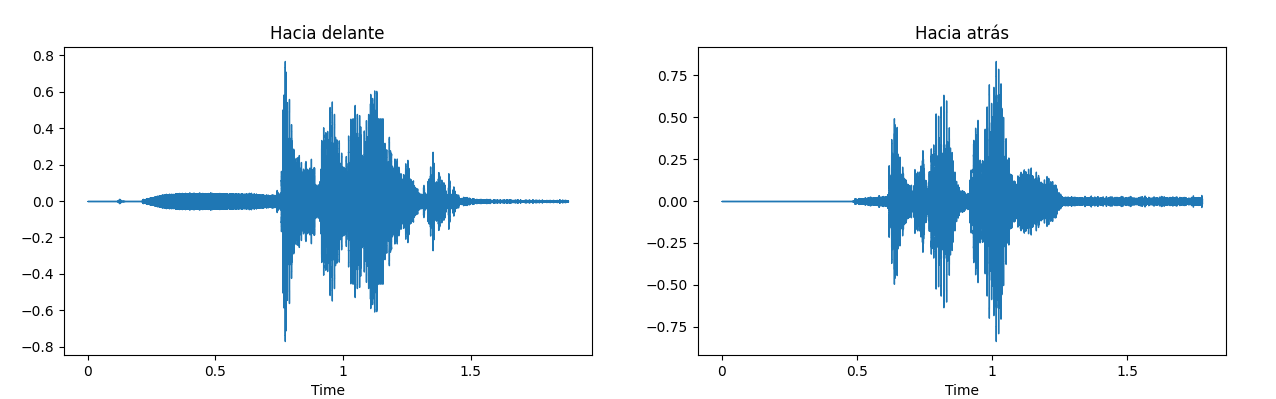
\includegraphics[scale=0.3]{figs/forma_onda} % Escala la imagen al 150% de su tamaño original
  \caption{ Forma de onda de diferentes audios.}
  \label{fig:onda}
\end{figure}



Para calcularla basta con abrir el archivo y leer los datos de audio en formato \texttt{float32} que es un formato estándar para procesar señales de audio. De esta manera, convierte la señal en un array en la que cada elemento representa la amplitud del audio guardado en \texttt{waveform}. También se calcula la frecuencia de muestreo que será necesaria para después.

\begin{verbatim}
with soundfile.SoundFile(file) as audio:
        waveform = audio.read(dtype="float32")
        sample_rate = audio.samplerate
\end{verbatim}

Para calcular la STFT (Figura \ref{fig:stft}) se hace uso de la función \verb|feature_chromagram(waveform, sample_rate)|, la cual toma la forma de onda y la frecuencia de muestreo y calcula la STFT del audio que descompone la señal en sus componentes de frecuencia a lo largo del tiempo y toma su valor absoluto, teniendo así una matriz en la cual las columnas representan los frames de tiempo y las filas representan las frecuencias. Luego lo convierte en un cronograma (Figura \ref{fig:cronograma}) que mide la energía de cada una de las notas musicales presentes en el frame, siendo una matriz cambiando las filas que son las notas musicales con las columnas (frames) y finalmente calcula la media de cada columna teniendo así un vector de 12 componentes en la que cada elemento representa la energía media de una nota en todo el audio.


\begin{code}[H]
\begin{lstlisting}[language=Python]
def feature_chromagram(waveform, sample_rate):
    stft_spectrogram=np.abs(librosa.stft(waveform))
    chromagram=np.mean(librosa.feature.chroma_stft(S=stft_spectrogram, sr=sample_rate).T,axis=0)
    return chromagram
\end{lstlisting}
\caption[Función para calcular la STFT de un audio]{Función para calcular la STFT de un audio}
\label{cod:codejemplo6}
\end{code}

\begin{figure}[H]
  \centering
  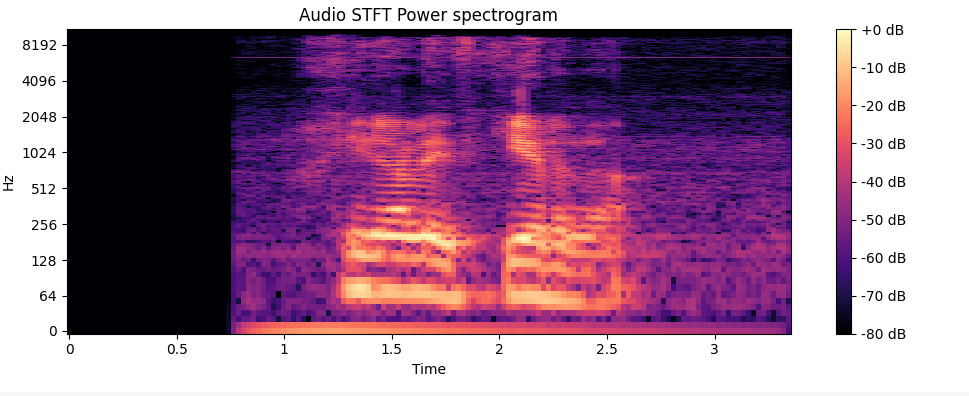
\includegraphics[scale=0.4]{figs/stft_spectogram} % Escala la imagen al 150% de su tamaño original
  \caption{ Representación de la transformada de Fourier de corta duración de un audio.}
  \label{fig:stft}
\end{figure}

\begin{figure}[H]
  \centering
  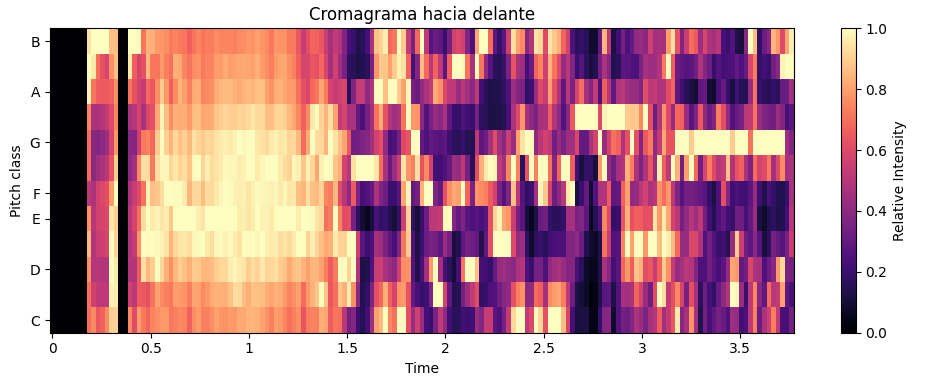
\includegraphics[scale=0.4]{figs/cromagrama} % Escala la imagen al 150% de su tamaño original
  \caption{ Representación del cronograma de un audio.}
  \label{fig:cronograma}
\end{figure}


Con la forma de onda y la frecuencia de muestreo, también se puede calcular los coeficientes MFCC (Figura \ref{fig:mfcc}) que nos dan una idea del tono cambiante de una señal de audio. Con la función \verb|feature_mfcc(waveform, sample_rate)|, se calculan los MFCCs de una señal y en este caso como indica el parámetro \texttt{n\_mfcc} se calculan 40 coeficientes para tener más detalles del contenido espectral, ya que para esta tarea 40 coeficientes proporcionan la mejor precisión y un cálculo rápido. \texttt{.T} transpone la matriz intercambiando así los coeficientes con los fotogramas de tiempo y luego se calcula la media de cada columna generando así un vector de tamaño 40.


\begin{code}[H]
\begin{lstlisting}[language=Python]
def feature_mfcc(waveform, sample_rate):
    mfc_coefficients=np.mean(librosa.feature.mfcc(y=waveform, sr=sample_rate, n_mfcc=40).T, axis=0)
    return mfc_coefficients
\end{lstlisting}
\caption[Función para calcular los espectrogramas mel de un audio]{Función para calcular los espectrogramas mel de un audio}
\label{cod:codejemplo5}
\end{code}

\begin{figure}[H]
  \centering
  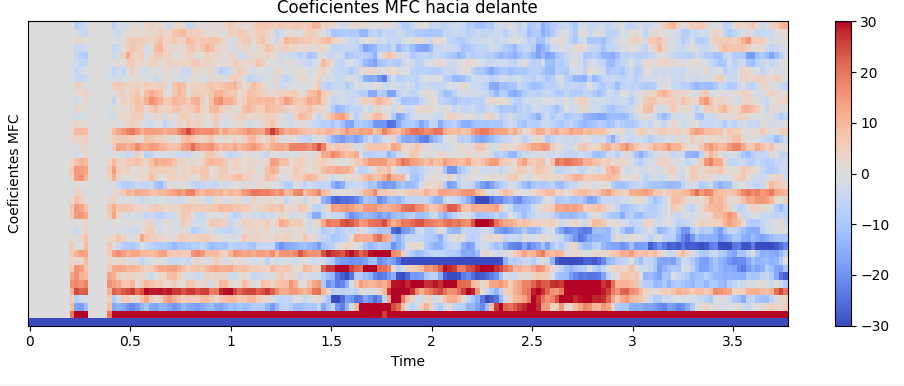
\includegraphics[scale=0.4]{figs/coeficientes_mfc} % Escala la imagen al 150% de su tamaño original
  \caption{ Representación de los coeficientes MFCC de un audio.}
  \label{fig:mfcc}
\end{figure}

Como derivado de los cálculos anteriores se pueden calcular los espectrogramas mel (Figura \ref{fig:mel}) que serán otra buena función para observar cómo son las transiciones entre los picos de frecuencias mel. Con la función \verb|feature_melspectrogram(waveform, sample_rate)|, se consiguen las características en forma de espectrograma mel el cual se asemeja cómo los humanos perciben las frecuencias. \texttt{N\_mels} se corresponde con el número de bandas en la escala mel con lo que se genera un espectrograma con 128 características y \texttt{f\_max} es la frecuencia máxima y para la mayoría de tareas de clasificación por voz 8kHz es suficiente. \texttt{.T} transpone la matriz del espectrograma mel intercambiando así las bandas mel(filas) con los fotogramas de tiempo(columnas) y luego se calcula la media de cada columna generando así un vector de tamaño 128 en la que cada valor representa la energía media de una banda mel.



\begin{code}[H]
\begin{lstlisting}[language=Python]
def feature_melspectrogram(waveform, sample_rate):
    melspectrogram=np.mean(librosa.feature.melspectrogram(y=waveform, sr=sample_rate, n_mels=128, fmax=8000).T,axis=0)
    return melspectrogram
\end{lstlisting}
\caption[Función para calcular los espectrogramas mel de un audio]{Función para calcular los espectrogramas mel de un audio}
\label{cod:codejemplo5}
\end{code}

\begin{figure}[H]
  \centering
  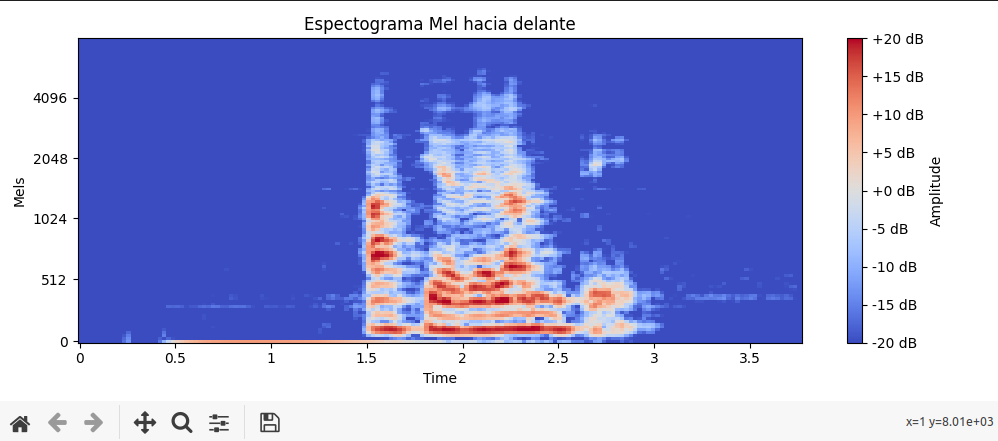
\includegraphics[scale=0.4]{figs/mel_spectrogram} % Escala la imagen al 150% de su tamaño original
  \caption{ Representación de los espectrogramas mel de un audio.}
  \label{fig:mel}
\end{figure}

Ya con todo esto se tendrían 180 características, de las cuales 128 pertenecerían al número de bandas mel que se utilizan para calcular el espectrograma mel, ya que se ha establecido en 128 porque funciona óptimamente,ya que valores más altos pueden proporcionar una representación más detallada pero también pueden requerir más recursos computacionales. Otras 40 saldrían de establecer 40 MFCC, aunque al igual que el anterior parámetro no hay un número fijo. Las otras 12 restantes serían las del cromagrama, una para cada una de las 12 clases de tonos.

Una vez calculadas las 180 características para cada uno de los audios se agruparán en una matriz los audios totales que haya en el dataset para poder representarlos correctamente de esta manera:

\begin{verbatim}
feature_matrix = np.hstack((chromagram, melspectrogram, mfc_coefficients))
\end{verbatim}

Como estas características tienen magnitudes diferentes, es necesario escalarlas para normalizar los datos y que las características tengan una escala comparable, mejorando así la estabilidad y el rendimiento del modelo, ya que se obtenía que la desviación de los coeficientes MFCC era mayor que la de las demás características. 

Para el escalado se usó la función \verb|StandardScaler()| de sklearn que resta la media de cada característica y la divide por la desviación estándar de esa característica, produciendo características con media cero y varianza unitaria, por lo que los valores extremos tendrán menos impacto en los pesos aprendidos del modelo y el modelo es menos sensible a los valores atípicos. 

El siguiente paso sería elegir el modelo que se va a usar y como se podrá observar más adelante, se usará el modelo Random Forest para entrenar a la red ya que en este experimento \ref{sec:eleccion_modelo}, se observó el rendimiento de cada uno de los modelos y el más fiable era el de RandomForestClassifier, junto con la clasificación por vectores de apoyo SVC.

El proceso final sería cargar el modelo ya entrenado, ejecutar mediante el módulo \texttt{subprocess} el comando arecord para grabar un audio, obtener las características del audio y pasárselas al modelo para que haga la predicción correcta en la respectiva clase del audio al que pertenece. El comando arecord tiene diferentes parámetros como los siguientes: 

\begin{verbatim}
arecord -t wav -d 2 -r 44000 -c 1 ej20-01-.wav 
\end{verbatim}

El parámetro -t wav especifica el tipo de archivo de audio como WAV, -d 2 establece la duración de la grabación en 2 segundos, -r establece la frecuencia de muestreo en 44,000 Hz, -c 1, especifica que se desea grabar con un solo canal (mono). Esto último es importante ya que en este caso solo se usa un canal para transmitir el sonido y si se graba como -c 2 se estará usando un canal estéreo que usa dos canales por lo que al pasárselo a la red dará problemas.


\subsection{Localización}
\label{subsec:localización}

Al navegar en interiores, la tecnología GPS no es adecuada para esta tarea ya que la señal es débil y puede proporcionar un error muy alto, por lo que se ha usado un sistema de posicionamiento basado en la utilización de balizas WiFi para obtener una estimación de la posición del robot mediante los valores RSSI para obtener la distancia y con la posición en la que se ubican en el mapa los APs. Para conectarse a un AP se utilizará esta función \ref{cod:codejemplo6}, en la cual se usa el comando \texttt{subprocess.run} para ejecutar \texttt{nmcli} especificando la red(en este caso WiFi), la acción para conectarse a ella junto con el nombre de la red y la contraseña y con \texttt{check=True} hace que se genere una excepción si falla el comando.\\

\begin{code}[H]
\begin{lstlisting}[language=Python]
def connect_to_wifi(ssid, password):
    try:
        subprocess.run(["nmcli", "d", "wifi", "connect", ssid, "password", password], check=True)
        print(f"Conectado a {ssid}")
    except subprocess.CalledProcessError as e:
        print(f"Error al conectar a {ssid}: {e}")
\end{lstlisting}
\caption[Función para conectarse a una red WiFi]{Función para conectarse a una red WiFi}
\label{cod:codejemplo6}
\end{code}

Una vez se tiene la potencia recibida del AP, para calcular la distancia hay que usar esta ecuación \ref{ec:ec2}:




\begin{myequation}[H]
\begin{equation}
d = 10^{\frac{A - \texttt{RSSI}}{10 \cdot n}}
\label{ec:ec2}
\end{equation}
\caption[Ecuación para calcular la distancia a un AP]{Ecuación para calcular la distancia a un AP}
\end{myequation} 
\texttt{Donde:}
\begin{itemize}
    \item $d$: Distancia estimada en metros.
    \item $A$: Valor RSSI a 1 metro del AP.
    \item \texttt{RSSI}: Potencia recibida.
    \item $n$: Factor de propagación (depende del entorno, generalmente es 2-3 en interiores).
\end{itemize}


Teniendo ya la distancia a cada AP y sabiendo la posición de cada uno de ellos en el mapa, mediante múltiples puntos de referencia se puede usar la trilateración y calcular la posición del robot. Para ello se puede usar este sistema de ecuaciones \ref{ec:ec5}. 




\begin{myequation}[H]
\begin{equation}
\left\{
	\begin{array}{lcc}
		(x - x_1)^2 + (y - y_1)^2 = (d_1)^2\\
		(x - x_2)^2 + (y - y_2)^2 = (d_2)^2\\
		(x - x_3)^2 + (y - y_3)^2 = (d_3)^2 \\
		(x - x_4)^2 + (y - y_4)^2 = (d_4)^2
	\end{array}
\right.
\label{ec:ec5}
\end{equation}
\caption[Sistema de ecuaciones para calcular la posición dada la distancia y la posición de cada AP]{Sistema de ecuaciones para calcular la posición dada la distancia y la posición de cada AP}
\end{myequation}


El siguiente paso sería averiguar cuántos APs son necesarios para estimar la posición y que haya el mínimo de error. Para ello se realizará un experimento \ref{sec:num_aps} en el cual se comprobará esto último y también se hará un estudio sobre el impacto que tiene el espacio que hay entre las cuadrículas del mapa sobre el cálculo de la posición del robot.


\subsection{Navegación}
\label{subsec:navegación}

Un problema a tratar es la navegación, y al tener una batería tan limitada no se puede hacer que se desplace grandes distancias, por lo que se tratará la navegación en interiores. En cuanto a la navegación global, es necesario implementar un algoritmo de navegación óptimo como el de A*. Este algoritmo combina características de los algoritmos de búsqueda de costo uniforme y búsqueda heurística, lo que lo hace eficiente y efectivo en la resolución de problemas de planificación de rutas. 

Dada una lista de datos o valores, este algoritmo buscará iterativamente los datos requeridos o
valor solicitado dentro de la lista, en este caso la matriz de 0 y 1 como se mencionó anteriormente. 

Después de considerar los criterios de compensación de optimalidad, completitud, precisión y el tiempo de ejecución, se ha determinado que el algoritmo de planificación de rutas A*
sería el más adecuado para el entorno simulado que se quiere probar. 


A* es lo que se considera un algoritmo de búsqueda Best-First, lo que significa que se tomará el movimiento de menor costo por iteración. Esto significa que se elige la ruta más cercana y eficiente que sea inmediatamente visible, analizando todos los posibles caminos más cortos. A* siempre encontrará una solución si existe una, lo que lo convierte en un algoritmo de búsqueda óptimo. Este algoritmo pretende minimizar el coste del camino cogido mediante la ecuación:


\begin{myequation}[H]
\begin{equation}
\left\{
	f(n) = g(n) + h(n)
\right.
\label{ec:ec6}
\end{equation}
\caption[Fórmula de la función de costo]{Fórmula de la función de costo}
\end{myequation}


Donde g(n) es el costo de cada movimiento desde el nodo inicial hasta el nodo final, y h(n) es la
heurística en la que se estiman los costos futuros. La heurística es una estimación o evaluación del costo de
movimientos futuros. Al sumar el costo estimado de los movimientos futuros y los pasos ya realizados, se puede estimar el camino de menor costo a recorrer.


El proceso final consistiría entonces en pasarle al algoritmo la imagen binaria del mapa de 0 y 1 y transformarla en una matriz con la cual trabajará el algoritmo, junto con el punto de partida y el objetivo final. Para encontrar el camino se verifica primero si el origen y el destino son válidos y si el punto inicial ya es el destino finaliza. Luego, se define la celda de inicio con los costos y la heurística a 0 dentro de otra matriz de objetos y se agrega a la cola de prioridad junto con sus coordenadas. En el bucle principal se sacará el nodo con menor f(n) de la cola de prioridad y expandiendo así el nodo con menor costo total y marcándola como visitada para no volver a procesarla. Después de esto se seguirán expandiendo los nodos vecinos y actualizando los costos y agregándolos a la cola de prioridad hasta encontrar el destino.

\begin{figure}[H]
  \centering
  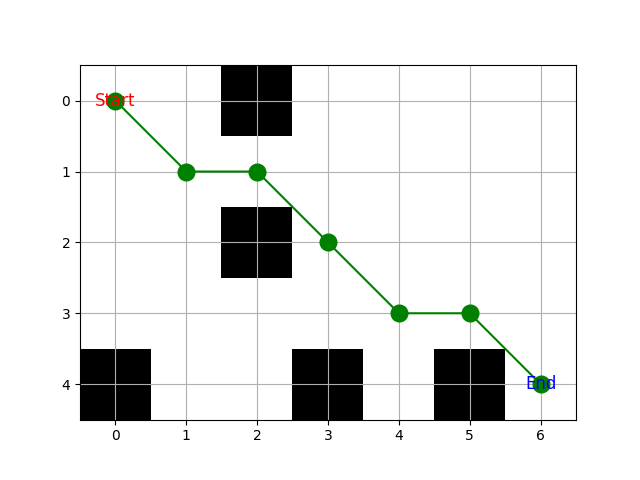
\includegraphics[scale=0.6]{figs/astar4} % Escala la imagen al 150% de su tamaño original
  \caption{ Ejemplo de búsqueda hacia un objetivo con A*.}
  \label{fig:mel}
\end{figure}



\chapter{Experimentos}
\label{cap:capitulo6}

\begin{flushright}
\begin{minipage}[]{10cm}
\emph{El único modo de hacer un gran trabajo es amar lo que haces}\\
\end{minipage}\\

Walter Isaacson, \textit{Steve Jobs}\\
\end{flushright}

\vspace{1cm}

Escribe aquí un párrafo explicando brevemente lo que vas a contar en este capítulo, que básicamente será una recapitulación de los problemas que has abordado, las soluciones que has prouesto, así como los experimentos llevados a cabo para validarlos. Y con esto, cierras la memoria.

\section{Conclusiones}

Enumera los objetivos y cómo los has cumplido.\\



\section{Calibración magnética}
\label{sec:cal_mag}

Una vez obtenido el ángulo de orientación,  es necesario tener en cuenta 3 aspectos. Como vivimos en una época en la que estamos rodeados de material magnético y de campos magnéticos inducidos por los dispositivos electrónicos que nos rodean, como los teléfonos y ordenadores, es necesario eliminar las fluctuaciones que estas variables pueden provocar en este experimento.\\

\subsection{Sesgo de Hard Iron}
\label{subsec:hard_iron}

El sesgo de Hard-Iron se refiere a un tipo de error sistemático causado por la presencia de un campo magnético fijo, como el de la Tierra o materiales ferromagnéticos cercanos como piezas metálicas, imanes, dispositivos electrónicos... que pueden distorsionar las lecturas del magnetómetro. Esto se puede corregir restando un valor de compensación fijo de las lecturas del MPU9250, que se puede determinar calibrándolo en un entorno de campo magnético conocido.

Antes de empezar con la calibración, se debe asegurar que el sensor se encuentra en una superficie plana horizontal. Primero se nos pedirá rotar el sensor 360º en los 3 ejes para obtener las medidas y visualizar la respuesta magnética de los sensores del magnetómetro.

Es fácil ver la gran variabilidad entre los tres planos del sensor antes de la compensación por el efecto del Hard-Iron. La rotación de 360° del sensor alrededor de cada eje debería producir un círculo centrado alrededor del origen ya que así se demuestra que se han eliminado los sesgos y está correctamente alineado, que se aprecia después de la compensación por los efectos del Hard-Iron como se puede apreciar en esta figura \ref{fig:hardiron}.

Los efectos del Hard-Iron primero deben restarse de los valores del magnetómetro que se están leyendo, ya que aumentará la precisión y la estabilidad de la aproximación de la orientación que se utiliza para esta aplicación de IMU.

\begin{figure}[H]
  \centering
  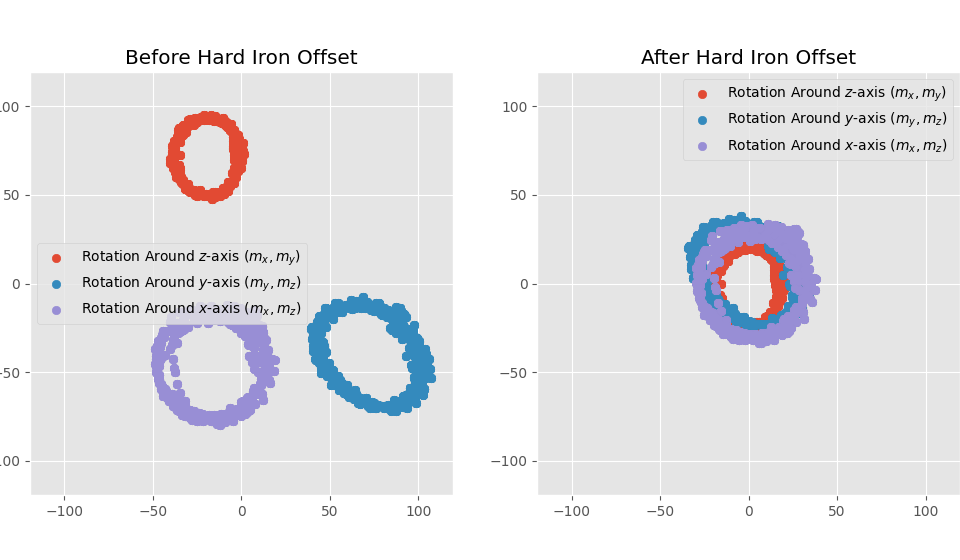
\includegraphics[scale=0.6]{figs/hard_iron_calibration} % Escala la imagen al 150% de su tamaño original
  \caption{ Representación de los efectos del sesgo de Hard Iron corregidos.}
  \label{fig:hardiron}
\end{figure} 

\subsection{Sesgo de Soft Iron}
\label{subsec:soft_iron}

Como se puede ver en la imagen, todavía hay algo de distorsión, así que se verá qué hace la eliminación del sesgo de Soft Iron.

Este sesgo es causado por la presencia de un campo magnético no uniforme, como la distorsión del campo magnético de la Tierra por objetos cercanos. Esto puede provocar que las lecturas del magnetómetro se desvíen hacia una dirección o eje particular y se puede corregir mediante un proceso de calibración que implica girar el sensor en un espacio 3D y recopilar datos del magnetómetro, que se pueden utilizar para calcular valores de corrección que se pueden aplicar a las lecturas del magnetómetro para compensar el campo magnético no uniforme.

El primer paso entonces será guardar los datos ya calibrados previamente antes en un archivo y se leerá de la entrada estándar, escalando así cada eje del magnetómetro obteniendo los factores de escala de cada eje para garantizar que la forma de rotación de la IMU mantenga su forma circular y si hay Soft-Iron presente, la rotación de la IMU producirá una respuesta más elíptica en lugar de circular y se obtendrán unos factores de escala los cuales habrá que multiplicar a los valores ya calibrados previamente. Como se puede ver en la imagen \ref{fig:softiron}, sigue teniendo una forma circular muy parecida por lo que se demuestra que no hay apenas Soft Iron presente, ya que sino tendría una respuesta más elíptica.

\begin{figure}[H]
  \centering
  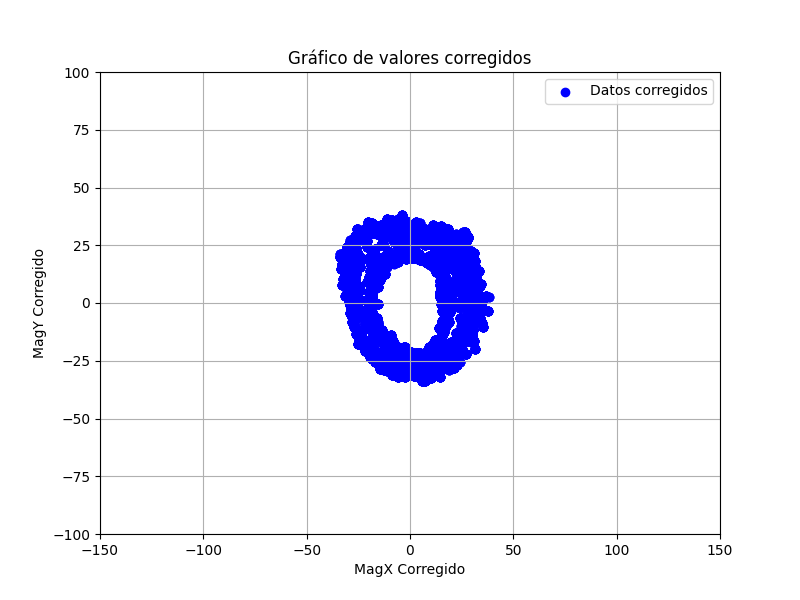
\includegraphics[scale=0.6]{figs/soft_iron_calibration} % Escala la imagen al 150% de su tamaño original
  \caption{ Representación de los efectos del sesgo de Soft Iron corregidos.}
  \label{fig:softiron}
\end{figure} 

\subsection{Filtro de paso bajo}
\label{subsec:filtro_paso_bajo}

A pesar de la calibración, todavía se pueden obtener más fluctuaciones como picos aleatorios en las lecturas magnéticas y no se busca que estas fluctuaciones nos desvíen de la señal buscada que es el campo magnético de la Tierra. Para lidiar con estos picos se implementará un filtro de paso bajo sobre los valores ya calibrados previamente con esta función \ref{cod:codejemplo5}:

\begin{code}[H]
\begin{lstlisting}[language=Python]
def low_pass_filter(valor_previo, nuevo_valor):
    return 0.85 * valor_previo + 0.15 * nuevo_valor
\end{lstlisting}
\caption[Función para aplicar un filtro de paso bajo]{Función para aplicar un filtro de paso bajo}
\label{cod:codejemplo5}
\end{code}


Como se puede ver, los pesos de este filtro suman 1 (0,85 + 0,15) y debe ser de esta manera ya que la premisa es que se confíe más en el valor anterior que en el nuevo. De esta manera se puede eliminar o reducir este ruido y mejorar la calidad de la medición de la señal del magnetómetro. Si se hubiese dado un peso mayor al dato nuevo, el filtro será más sensible a los cambios recientes, y con un peso más bajo los cambios serán más lentos pero se priorizará la estabilidad que es lo que se busca.

\section{Elección del modelo de aprendizaje automático}
\label{sec:eleccion_modelo}

Para elegir el modelo que se va a usar para entrenar a la red, hay que observar el rendimiento de cada uno de los modelos y seleccionar el más fiable para un datasets de audios. En este experimento se usó un dataset diferente que no es el mismo que se usará en la prueba final del robot, ya que al final se probará solo con varias clases y en este hay más, pero servirá para tener en cuenta la precisión de cada modelo. \\

Una vez se tienen las características escaladas como se mencionó anteriormente, hay que usar la función del módulo sklearn.model\_selection \verb|train_test_split(features_scaled, directions, test_size,random_state)| para dividir el conjunto de datos en conjuntos de prueba y entrenamiento. El primer parámetro son las características una vez estén escaladas, el segundo corresponde al conjunto de etiquetas o clases asociadas a un comando de voz, el tercero representa el porcentaje que va para las pruebas(siendo el porcentaje restante para entrenamiento) y el último debe ser un número entero cualquiera para que siempre se genere los mismos subconjuntos, ya que si es None o no se especifica, cada vez que se ejecute el código se dividirán de manera diferente y lo que se busca es que sea determinista y que no cambie con cada ejecución. El modelo se prueba en el 80\% de los datos y se prueba su rendimiento en el 20\% de los datos, que nunca ha visto en el entrenamiento. Esta función devuelve el conjunto de características para prueba y entrenamiento que es lo que se busca y también devuelve las etiquetas correspondientes a las características para entrenamiento y prueba que no se tendrán en cuenta ya que no son necesarias.\\

El siguiente paso sería evaluar los diferentes modelos de clasificación, iterando sobre cada uno de ellos, entrenando cada modelo con los datos de entrenamiento y calculando la precisión de cada uno en los datos de prueba. Como se puede apreciar en la figura \ref{fig:modelos}, se puede observar que el modelo más fiable sería RandomForestClassifier y la clasificación por vectores de apoyo SVC. Finalmente se usrará el primer modelo, ya que los bosques aleatorios son modelos excelentes para utilizar como referencia debido a su baja complejidad de tiempo de entrenamiento y a su robustez frente a distribuciones desconocidas y valores atípicos en el conjunto de datos.

\begin{figure}[H]
  \centering
  \includegraphics[scale=0.6]{figs/modelos} % Escala la imagen al 150% de su tamaño original
  \caption{ Precisión de cada modelo.}
  \label{fig:modelos}
\end{figure} 

\section{Elección del número de APs}
\label{sec:num_aps}

Para averiguar cuántos APs son necesarios para estimar la posición del robot y que haya el mínimo de error, antes es necesario probar el sistema en cuatro escenarios de prueba donde se evaluaron dos hipótesis diferentes:

\begin{enumerate}
 \item \textit{} ¿La precisión de las IPS Wi-Fi HaLow escala linealmente con el número de balizas?
 \item \textit{} ¿La precisión aumenta cuando la distancia mínima entre dos posiciones del grid es de 1 metro mientras que el área de mapeo no cambia?
\end{enumerate}\


Este experimento se probará en una habitación dividida en cuadrículas de 4x4 y se partirá de la base:

\begin{itemize}
\item \textit{} Las balizas BLE no se moverán de su posición durante la fase de entrenamiento y prueba.
 \item \textit{} 140 muestras por cada punto de cuadrícula son suficientes para capturar la dinámica RSSI(Al principio se probó con 180 muestras pero luego se probó con 140 y no cambiaban apenas los resultados).
 \item \textit{} La interferencia de WiFi y otras señales BLE se tendrán en cuenta.
 \item \textit{} Los escenarios de prueba realizados con 2 nodos, 3 nodos y 4 nodos son suficientes para responder a la hipótesis 1.
 \item \textit{} Para todos los escenarios, el dispositivo receptor deberá poder detectar todas las balizas WiFi presentes.
 \item \textit{} Entre cada punto del grid habrá una separación de medio metro.
\end{itemize}\


Esta imagen \ref{fig:escenario} muestra el entorno experimental para este proyecto.

\begin{figure}[H]
  \centering
  \includegraphics[scale=0.15]{figs/escenario} % Escala la imagen al 150% de su tamaño original
  \caption{ Entorno experimental.}
  \label{fig:escenario}
\end{figure} 

A continuación se mostrará los cuatro escenarios de prueba con detalles adicionales:




\begin{figure}[H]
    \centering
    % Primera fila de imágenes
    \begin{minipage}[b]{0.45\textwidth}
        \centering
    \includegraphics[width=6.5cm]{figs/dos_apes.png}
        \caption{Pimer escenario de prueba}
        \label{fig:escenario1}
    \end{minipage}
    \hfill
    \begin{minipage}[b]{0.45\textwidth}
        \centering
    \includegraphics[width=6.5cm]{figs/tres_apes}
        \caption{Segundo escenario de prueba}
        \label{fig:escenario2}
    \end{minipage}
    
    \vspace{1cm} % Espacio entre filas
    
    % Segunda fila de imágenes
    \begin{minipage}[b]{0.45\textwidth}
        \centering
    \includegraphics[width=6.5cm]{figs/cuatro_apes}
        \caption{Tercer escenario de prueba}
        \label{fig:escenario3}
    \end{minipage}
    \hfill
    \begin{minipage}[b]{0.45\textwidth}
        \centering
    \includegraphics[width=6.5cm]{figs/cuatro_apes_espaciados}
        \caption{Cuarto escenario de prueba}
        \label{fig:escenario4}
    \end{minipage}
\end{figure}


Esta sala de pruebas se toma como un cuadrado de 1,5 metros por 1,5 metros, marcado en un piso de madera. B1,B2,B3 y B4 representan las balizas de proximidad. En este caso se elegirán iPhones que mediante la transmisión de datos móviles, se conectarán a la Raspberry y servirán como puntos de acceso.

Cada una de las marcas grises marcadas en el suelo representa un punto de la cuadrícula etiquetado del 1 al 16. Cada uno de los números ordinales marcados aquí es una “etiqueta de clase” que el modelo tiene que predecir después del “entrenamiento” con los datos recopilados.

Para entender cómo se usa esto para estimar la posición, se presenta la analogía de un “faro”. Un faro proyecta una luz de intensidad fija en el océano. Un barco puede “estimar” su posición relativa con respecto al faro siguiendo la intensidad del haz de luz a medida que se acerca al faro. El mismo principio es aplicable para los valores RSSI. Si el receptor está cerca de la baliza, el valor es mayor y se reduce progresivamente a medida que el receptor se aleja.

Después de configurar los nodos y preparar el área de experimentación, se coloca la Raspberry Pi en cada uno de los puntos de la cuadrícula gris y se recolectan 140 muestras por punto. Esta tabla \ref{cuadro:tabla1} muestra un conjunto de datos de muestra para el escenario 1.


\begin{table}[H]
\begin{center}
\begin{tabular}{|c|c|c|c|}
\hline
\textbf{Index} & \textbf{B0} & \textbf{B1} & \textbf{Label}  \\
\hline
s1 & -59 & -36 & 1 \\  
s3 & -59 & -38 & 1 \\   
s3 & -54 & -37 & 1 \\   
\hline
\end{tabular}
\caption{Ejemplo de un conjunto de datos del escenario 1}
\label{cuadro:tabla1}
\end{center}
\end{table}


Aquí, \texttt{B0} y \texttt{B1} corresponden a la posición de los nodos \texttt{B1} y \texttt{B2} que se muestran en la figura del primer escenario (Figura \ref{fig:escenario1}). En términos de la jerga del aprendizaje automático, nuestros “vectores de características” son las columnas que corresponden al valor RSSI de un nodo, mientras que la columna “Etiqueta” es el resultado esperado.

Después de completar la recopilación de datos, se verifican los datos en busca de valores faltantes. Se encontró que aparecían valores como \texttt{None} en ciertas muestras. En estos casos, simplemente se copia el valor RSSI de la muestra anterior.

Los datos preprocesados se dividieron luego en una división de prueba y entrenamiento de 90\texttt{-}10. Después de eso, se aplicarán cuatro modelos de aprendizaje automático a los datos y se comparan los resultados para responder a las dos hipótesis establecidas. Los escenarios del 1 al 3 se utilizaron para responder la hipótesis 1 y, el escenario 4 se utilizó para responder la hipótesis 2.

Además, se utilizó una técnica de ajuste automático de hiperparámetros llamada GridSearchCV para buscar en el espacio de hiperparámetros de cada uno de los cuatro escenarios para obtener los mejores parámetros que se ajustan bien a los datos sin sobreajustarlos pasándole como parámetro el estimador que implementa la interfaz del estimador de scikit-learn y debe proporcionar una función de puntuación o debe pasarse la puntuación.

Ahora se probarán los diferentes modelos para cada escenario en una herramienta interactiva llamada Jupyter Notebook como ya se mencionó anteriormente en esta sección \ref{subsec:Jupyter} y se obtuvieron los siguientes resultados en esta tabla \ref{cuadro:tabla2} para los escenarios 1,2 y 3 respectivamente:


\begin{table}[H]
\begin{center}
\begin{tabular}{|c|c|c|c|c|}
\hline
\textbf{Nodos} & \textbf{SVC, Linear} & \textbf{SVC,RBF} & \textbf{DTREE} & \textbf{RF} \\
\hline
2 & 28\% & 31\% & 28\% & 24\% \\  
3 & 82\% & 86\% & 78\% & 82\% \\   
4 & 94\% & 94\% & 91\% & 94\% \\   
\hline
\end{tabular}
\caption{Resultados de los modelos para los primeros tres escenarios}
\label{cuadro:tabla2}
\end{center}
\end{table}


De la anterior tabla se deduce que la precisión de los cuatro modelos aumenta a medida que aumenta el número de nodos. Por lo tanto, se concluye que la hipótesis 1 es verdadera para el. Además, todos los modelos tuvieron un desempeño significativamente bueno en contraste con los anteriores. Sin embargo, aunque la mejor precisión es del 94%, aunque parezca suficiente no lo es, ya que se busca el 100% porque todo lo que no sea eso supondrá un error en la medición de la posición del robot y que por mínima que sea, puede afectar al posicionamiento del mismo.

Se atribuye este bajo número de precisión al hecho de que cada uno de los puntos de la cuadrícula está a solo 50 cm de distancia, mientras que la regla general común era separarlos entre sí por 1,5 ~ 2 metros. Esto provocó que los pares de puntos de la cuadrícula adyacentes tuvieran valores RSSI superpuestos, como se muestra en esta figura \ref{fig:vals1}:



\begin{figure}[H]
  \centering
  \includegraphics[scale=0.4]{figs/vals1} % Escala la imagen al 150% de su tamaño original
  \caption{ Representación de los valores RSSI en cada punto de la caudrícula para cada AP.}
  \label{fig:vals1}
\end{figure} 

Por lo tanto, se formula la hipótesis 2 para investigar el efecto de la separación de los puntos de la cuadrícula en la precisión de los clasificadores. Esta tabla \ref{cuadro:tabla2} muestra los resultados del escenario 4:

\begin{table}[H]
\begin{center}
\begin{tabular}{|c|c|c|c|c|}
\hline
\textbf{Nodos} & \textbf{SVC, Linear} & \textbf{SVC,RBF} & \textbf{DTREE} & \textbf{RF} \\
\hline
4 & 99\% & 99\% & 96\% & 100\% \\  
\hline
\end{tabular}
\caption{Resultados de los modelos para el cuarto escenario}
\label{cuadro:tabla2}
\end{center}
\end{table}


Cada uno de los modelos ha demostrado obtener una mejora significativa rozando la perfección en la precisión en comparación con el escenario 3. Por lo tanto, se concluye que la hipótesis 2 es verdadera. Se justifica esta mejora señalando que, con una cuadrícula de ubicación espaciada, hubo menos superposición de datos RSSI entre posiciones adyacentes como se puede apreciar en esta imagen \ref{fig:vals2} y por lo tanto mayor precisión en los modelos al clasificar los datos:

\begin{figure}[H]
  \centering
  \includegraphics[scale=0.4]{figs/vals2} % Escala la imagen al 150% de su tamaño original
  \caption{ Representación de los valores RSSI en una cuadrícula espaciada para cada AP.}
  \label{fig:vals2}
\end{figure} 

En este experimento se usó la banda de frecuencia 2.4835 GHz que es de las más utilizadas para las comunicaciones inalámbricas. Al solo disponer de Iphones, no se pudo cambiar a la banda de 5GHz para transmitir y así obtener mediciones más precisas ya que esta banda tiene menos congestión y menos interferencias ya que menos dispositivos tienden a usarla, lo que mejora la calidad de la señal, mientras que la de 2.4385 GHz, tiene mayor interferencia debido a la saturación de dispositivos que la utilizan esta banda (como microondas, teléfonos inalámbricos...), lo que puede afectar la calidad de la transmisión y es más susceptible a interferencias de otras redes Wi-Fi cercanas, ya que muchas redes en un área densa suelen operar en los mismos canales.

En este experimento se ha demostrado con éxito la aplicación de un sistema de posicionamiento en interiores utilizando balizas WiFi y modelos de aprendizaje automático. Se prueban dos hipótesis y se demuestran que eran verdaderas siempre que se tuvieran en cuenta ciertos supuestos.

Por último, se ha llegado a la conclusión de que 4 APs sería suficientes para obtener una localización decente del robot como se ha demostrado en la hipótesis 2.......ver el error en al posscion si es de 1 metro....




\section{Corrector ortográfico}

Una vez tengas todo, no olvides pasar el corrector ortográfico de \LaTeX a todos tus ficheros \textit{.tex}. En \texttt{Windows}, el propio editor \texttt{TeXworks} incluye el corrector. En \texttt{Linux}, usa \texttt{aspell} ejecutando el siguiente comando en tu terminal:

\begin{verbatim}
aspell --lang=es --mode=tex check capitulo1.tex
\end{verbatim}


\chapter{Conclusiones}
\label{cap:capitulo5}

\begin{flushright}
\begin{minipage}[]{10cm}
\emph{El talento es importante, pero la perseverancia es más importante.}\\
\end{minipage}\\

Angela Duckworth, \textit{Grit}\\
\end{flushright}

\vspace{1cm}

En este último capítulo se presentan los objetivos alcanzados y las conclusiones que se han obtenido, junto con las competencias, habilidades y conocimientos adquiridos durante el desarrollo de este proyecto, incluyendo además posibles líneas de trabajo futuras.


\section{Objetivos cumplidos}
\label{sec:objetivos_cumplidos}


Con el desarrollo de este proyecto se han logrado todos los objetivos establecidos en el Capítulo \ref{cap:capitulo3}. El objetivo principal era diseñar un robot móvil de bajo coste con piezas 3D que fuera capaz de moverse en interiores hacia un destino final mediante comandos de voz y que fuera capaz de localizarse mediante dispositivos Wi-Fi en un mapa establecido previamente. A su vez, el robot debía orientarse adecuadamente, navegar correctamente por el mapa detectando obstáculos y que el sistema fuera portable a otros entornos de la manera más sencilla posible y que todas estas características funcionasen en una CPU de baja capacidad de cómputo. Todo ello se ha conseguido de manera exitosa.\\


También se han alcanzado los objetivos específicos que se propusieron. Uno de ellos era entrenar una red neuronal de audios por voz para enseñar a la red a clasificar e interpretar las órdenes dadas por el usuario. Otro era conseguir que el robot se localizara en el mapa a partir de 4 dispositivos Wi-Fi.\\

En cuanto al resto de objetivos secundarios, se consiguió que el robot se orientase correctamente y que detectase obstáculos mediante el sensor MPU9250 y HC-SR04 respectivamente. Para conseguir que fuera portable a otros entornos, se usó la herramienta \hyperlink{GIMP}{GIMP} con la cual se puede diseñar el mapa binario de una manera fácil y sencilla y que el robot navegue por el mapa a partir de la matriz del mismo y del algoritmo de navegación A* para encontrar la ruta más corta de manera eficiente hacia el destino final. Por último, se consiguieron combinar todos los datos de navegación y localización mediante la librería threading a partir del control y la ejecución de diferentes hilos ejecutados en paralelo. Al usar una placa Raspberry Pi 4, se ha conseguido que el sistema implementado sea accesible económicamente para cualquier usuario.\\


La lectura de los sensores se ha ido volcando en una doble cola de tamaño 1 almacenando así el último valor y eliminando automáticamente los anteriores ya que si no se especifica el tamaño máximo de cola, puede llegar a consumir mucha memoria porque se generan muchos datos en poco tiempo.\\


Para saber cuántos dispositivos Wi-Fi usar, se probó el sistema en cuatro escenarios de prueba donde se evaluaron las hipótesis de si la precisión de las IPS Wi-Fi HaLow escalaba linealmente con el número de balizas y si la precisión aumentaba cuando la distancia mínima entre dos posiciones del grid aumentaba. Ambas hipótesis se confirmaron a partir de obtener numerosas muestras en cada punto del grid y de aplicar modelos de aprendizaje automáticos y comprobar cómo clasificaban los datos en función del número de dispositivos Wi-Fi.\\

Para conseguir que el robot realizase giros precisos, era necesario calibrar antes el dispositivo MPU9250 tendiendo en cuenta el error sistemático que se producía al haber materiales ferromagnéticos y campos magnéticos inducidos por los dispositivos electrónicos que nos rodean. A pesar de la calibración, todavía se podían obtener más fluctuaciones como picos aleatorios en las lecturas y para lidiar con estos picos se implementó un filtro de paso bajo sobre los valores ya calibrados.\\

Este trabajo de fin de grado supone un avance respecto a los robots guía convencionales, los cuales son generalmente caros y difíciles de adaptar a diferentes entornos debido a todos los cambios que serían necesarios a nivel de software y esto supondría un gasto de tiempo importante. Una de las limitaciones del sistema es que al aumentar el número de dispositivos Wi-Fi para localizarse, aumenta el tiempo de respuesta para avanzar de una posición a otra y llegar al objetivo final.\\


Durante la realización del trabajo, se han obtenido conocimientos sobre diferentes habilidades y temas, entre los que se incluyen los siguientes:

\begin{itemize}

 \item \textit{} Adquisición de mayor experiencia y conocimientos sobre nuevas librerías y funciones para la programación en Python.
 \item \textit{} Conocimiento de herramientas de manipulación de imágenes como GIMP.
 \item \textit{} Mayor experiencia y conocimientos sobre el entrenamiento y funcionamiento de redes neuronales.
  \item \textit{} Conocimientos sobre la calibración de sensores como el MPU9250.
   \item \textit{} Desarrollo de nuevas habilidades en Latex.
  \item \textit{} Conocimientos acerca del funcionamiento y características de piezas \textit{hardware} como el controlador L298N o los motores.
  \item \textit{} Conocimientos sobre la aplicación de modelos de aprendizaje automático para distintas aplicaciones.
  \item \textit{} Conocimientos sobre cómo manejar y controlar la Raspberry a distancia desde otros dispositivos como ordenadores sin cables de por medio.
  
\end{itemize}\


\section{Líneas futuras}
\label{sec:lineas_futuras}

En esta sección se comentan algunas vías para permitir la continuidad de este trabajo y añadir funciones que aún no están disponibles para mejorar el funcionamiento del sistema presente:

\begin{itemize}

 \item \textit{} El modelo usado para entrenar la red neuronal para clasificar los comandos de voz tiene sobreajuste (overfitting), que ocurre cuando se ajusta demasiado bien a los datos debido a que el dataset es pequeño ya que solamente tiene dos clases. Para solucionarlo, habría que usar más datos de entrenamiento para más clases diferentes y con distintas voces de diferentes personas y edades.
 
 \item \textit{} Usar dispositivos Smartphones en lugar de iPhones, ya que los segundos usan la banda de frecuencia 2.4835 GHz que tiene mayor interferencia debido a la saturación de dispositivos que la utilizan y no se pueden cambiar a la banda de 5 GHz ya que esta banda tiene menos congestión y menos interferencias porque menos dispositivos tienden a usarla, lo que mejora la calidad de la señal, mientras que los primeros sí pueden cambiarse a esta banda.
 \item \textit{} Probar este sistema en áreas de mayor tamaño y con más dispositivos Wi-Fi para poder localizarse el robot.
  \item \textit{} Usar dispositivos Bluetooth para comparar la precisión respecto a los dispositivos Wi-Fi.
  \item \textit{} Añadir un altavoz para que el robot se pueda comunicar con el usuario y mantener conversaciones más fluidas sobre a qué lugar le gustaría ir el usuario para que el robot pueda guiarle correctamente.
 \item \textit{} Conseguir que el robot genere nuevas rutas en el caso de que las haya, cuando detecta un obstáculo como una persona y no se mueve durante mucho tiempo, ya que en este sistema hasta que no se moviera el obstáculo, el robot no avanza.
\end{itemize}\





\clearpage
\thispagestyle{empty}

\printindex \nocite{*}
\appendix
\bibliographystyle{apalike} \bibliography{bibliografia}

\end{document}
